\documentclass[UTF8]{heuthesis}

\usepackage{fontspec}
\setmainfont{Times New Roman}
\setsansfont{Arial}
\setmonofont{Consolas}
\usepackage{xurl}
\usepackage{enumitem}
\setlist{nosep}
\hypersetup{hidelinks}

\thesisTitle{基于树莓派的人脸识别考勤系统设计与实现}
\authorName{陈浩}
\studentID{2022201616}
\advisor{吕继光}
\majorField{软件工程}
\collegeName{计算机科学与技术学院}
\submitDate{2026年6月}

\begin{document}
\makeCover

\frontmatter
\chapter*{摘\quad 要}
\addcontentsline{toc}{chapter}{摘\quad 要}
实验室、课程签到和小型办公场所的考勤人数一般不算特别大，但记录又不能完全随意处理。传统人工签到、纸质登记和刷卡方式实现起来并不复杂，真正使用时却常遇到排队、代签、补录麻烦和后期统计不方便等问题。结合本次毕业设计的硬件条件，本文把摄像头采集、身份识别和签到写入尽量放在树莓派端完成，设计并实现了一套面向小规模场景的人脸识别考勤系统。

系统后端采用FastAPI，主要负责终端页面、用户门户、动作挑战和管理员接口；页面由Jinja2模板渲染，基础样式使用Bootstrap完成。数据保存采用SQLite，成员名单、用户账号、人脸档案、审核记录和考勤流水都落在本地数据库中。识别部分经过对比后选用OpenCV YuNet进行人脸检测，使用SFace提取特征并计算余弦相似度，终端活体判断则由OpenVINO加载anti-spoof-mn3模型完成。围绕注册和签到两条流程，系统实现了名单导入、首次注册改密、动作挑战抓拍、注册照质量校验、管理员审核、终端实时识别、签到写库和远程管理接口。注册端采用正脸、侧转、再正脸的三步挑战，并加入姿态、同人一致性、模糊度、亮度和翻拍风险检查；终端端将摄像头采集和识别推理拆成两个线程，识别线程只处理最新帧，再按照单人入镜、人脸面积、活体、身份匹配、考勤时间窗和重复签到冷却等条件逐步判断。

测试阶段主要检查了用户注册、人脸提交、管理员审核、终端签到和记录查询等流程。测试库能够保存成员名单、审核通过的人脸档案和考勤记录；终端采集分辨率为1280×720，摄像头采集目标为15FPS，识别线程目标为5FPS。在实验室门口这类单人依次通过的场景下，系统可以给出实时反馈并写入签到记录。受硬件和项目规模限制，当前版本仍以单台树莓派和小规模人脸库为主，后续还需要继续补充多终端同步、考勤规则配置和统计报表等功能。


\par\noindent{\heiti 关键词：}人脸识别，树莓派，考勤系统，活体检测，边缘计算

\clearpage
\chapter*{ABSTRACT}
\addcontentsline{toc}{chapter}{ABSTRACT}
In small laboratory, classroom, and office scenarios, attendance records are usually simple in scale but still need to be reliable enough for later checking. Manual sign-in, paper registration, and card-based attendance are easy to arrange, yet queues, proxy sign-in, manual statistics, and lost physical media often appear in actual use. Based on the hardware available in this graduation project, this thesis places camera capture, face recognition, liveness checking, and attendance writing on a Raspberry Pi terminal, and implements a lightweight face-recognition attendance system for local deployment.

The backend is built with FastAPI. Jinja2 templates and Bootstrap are used for the terminal page and the user portal, while SQLite stores roster members, users, face profiles, review history, and attendance records. For face recognition, the system uses OpenCV YuNet for face detection, SFace for feature extraction and cosine-similarity matching, and OpenVINO with the anti-spoof-mn3 model for passive liveness detection. The implemented workflow includes roster import, first-time registration, password change, action-challenge capture, face quality validation, administrator review, terminal recognition, attendance recording, and remote management APIs. During registration, the user completes a front-face, side-turn, and front-face-again challenge. At the terminal side, frame capture and recognition are separated into two threads, so recognition keeps working on the latest available frame instead of chasing old frames.

The test work checks the process from account activation to terminal check-in. The test database records roster members, approved face profiles, and attendance entries persistently. With 1280×720 camera input, 15 FPS capture, and a 5 FPS recognition target, the terminal can provide usable feedback in a laboratory-door check-in scenario. The current version is still designed around one Raspberry Pi and a small face database. Multi-device synchronization, configurable attendance rules, and statistical reports remain as future improvements.


\par\noindent{\bfseries Keywords:} Face recognition, Raspberry Pi, attendance system, liveness detection, edge computing
\clearpage
\tableofcontents
\clearpage
\mainmatter
\chapter{绪论}
\section{研究背景与意义}
在学校实验室和小型办公空间中，考勤记录往往不只是统计谁到了，还会和设备使用、安全责任以及异常追溯联系在一起。传统方式主要包括手工签到、纸质登记、IC卡和指纹识别。手工和纸质方式容易上手，但集中签到时经常需要排队，后续统计也要人工整理；IC卡依赖实体卡片，忘带、遗失和代刷都会影响记录可信度；指纹识别能减少代签，不过接触式采集会带来设备磨损和公共卫生方面的顾虑。

人脸识别通过摄像头采集用户面部图像，再经过人脸检测、特征提取和相似度匹配完成身份确认。它的优点比较直接：不需要用户携带卡片，也不需要接触设备。对考勤系统来说，这种方式可以减少签到动作，同时对代签、代刷一类问题形成一定约束。近几年轻量模型和边缘计算的发展，也让人脸检测、特征提取和活体检测有机会在树莓派这类低成本设备上运行，考勤终端不一定非要依赖高性能服务器。

本课题选用树莓派作为终端，主要是因为它体积小、功耗低，能够连接USB摄像头并运行Linux服务。对于实验室门口这类固定部署点，树莓派可以同时承担摄像头采集、模型推理、页面服务和SQLite本地存储。视频帧在端侧处理，能减少持续上传带来的带宽压力；成员照片和考勤记录保存在本地数据库中，也更符合小规模场景独立运行的需求。管理员需要查看设备时，再通过局域网或Tailscale访问管理接口即可。

面向实际使用的人脸考勤系统不能只做一次人脸比对。注册资料是否真实、终端识别是否及时、短时间内是否重复签到、照片或屏幕翻拍能否被拦截、管理员能否远程审核，这些都会影响系统能不能真正落地。因此，本文围绕树莓派端侧部署场景，设计并实现一套人脸识别考勤系统。系统以OpenCV YuNet和SFace作为主要识别链路，结合OpenVINO被动活体检测、动作挑战、人脸质量校验、审核流和管理员API，把成员名单导入、用户注册、审核、终端签到和记录查询串联起来。

\section{国内外研究现状}
国内关于考勤系统的研究已经不再停留在“记录一次签到”这一层面，很多工作开始把身份核验、统计查询、远程管理和场景联动放在一起讨论。周春杰将人脸识别与行人重识别用于考勤系统，尝试把人员跟踪和身份确认结合起来[1]。孙和杨国为面向学生考勤场景研究了人脸识别方案，田丽和李颖则在IPv6校园网络环境中设计了人脸识别考勤管理系统[2-3]。王维和杨路基于OpenCV与SQLite实现桌面端人脸识别考勤系统，对小规模本地视觉处理具有一定参考价值[4]。另外，徐源等和刘琼等分别从微信小程序角度设计门禁或学生考勤系统，说明移动端入口在校园管理中使用较多[5-6]。张雪倪将人脸识别考勤应用到国铁企业管理场景，也说明该类系统可以扩展到组织化人员管理中[7]。

在校园应用和嵌入式边缘部署方面，相关研究更关注低成本硬件、轻量模型和系统集成。张静分析了AI人脸识别在校园场景中的图像采集、定位、校准和比对问题[8]。高明等基于树莓派实现了人脸识别门禁系统，说明低成本开发板可以承担一定视觉识别任务[9]。赵洋和许军将MobileNetV2与树莓派结合用于人脸识别，重点解决端侧算力受限问题[10]。宋昌伟等设计了基于树莓派的人脸识别校园管理系统，为校园身份识别终端的集成提供了参考[11]。这些工作给本文提供了硬件和方案上的依据，但考勤系统还需要继续打通成员名单、注册审核、活体检测、端侧签到和后台查询等流程。

考勤系统还要面对照片、手机屏幕和预录视频等冒用风险。邓雄和王洪春从深度学习与特征融合角度研究人脸活体检测[12]，赵洋等讨论了多模态特征融合方法[13]，杨瑞杰和王洪春将InceptionV3与特征融合用于防伪判断[14]。这类研究提醒本文，考勤写库不能只看人脸相似度。结合树莓派部署条件，本文在注册端加入动作挑战和质量校验，在终端端加入被动活体检测与翻拍风险分析，使照片入库和现场签到都经过额外检查。

国外人脸识别方法大体经历了从人工特征到深度嵌入特征的变化。早期方法更多依赖主成分分析、局部二值模式等手工描述符，遇到光照、姿态和遮挡变化时稳定性有限。深度学习方法出现后，识别系统逐渐转向学习人脸嵌入向量。FaceNet使用三元组损失拉近同类样本、拉远异类样本[15]；ArcFace和CosFace通过角度间隔或余弦间隔增强特征区分度[16-17]。本文实现中直接采用可部署的SFace特征向量，完成小规模人脸库匹配。

人脸检测是识别流程的前置环节。Zhang 等提出的 MTCNN 将人脸检测和关键点定位结合起来，能够输出人脸框和关键点，广泛应用于注册质量校验和姿态估计场景[18]。近年来，端侧部署对模型体积和推理速度提出了更高要求。YuNet 面向轻量化人脸检测任务设计，能够在较小模型规模下输出人脸框与关键点信息，适合CPU设备上的实时检测[19]。SFace通过约束特征空间提升人脸特征的可分性和鲁棒性[20]，并可与OpenCV提供的检测和识别接口结合，形成可部署的人脸识别链路[21]。

活体检测是人脸识别系统安全性的重要组成部分。人脸考勤系统面对的攻击方式通常包括纸质照片、手机屏幕翻拍和预录视频等。活体检测方法可以分为主动式和被动式两类。主动式方法要求用户完成眨眼、摇头、张嘴等动作，再由系统判断动作是否真实；被动式方法不要求用户额外配合，而是利用纹理、反光、频域特征或生理信号进行判断。相关综述指出，深度学习活体检测方法需要同时关注跨设备、跨光照和跨攻击介质的泛化能力[22]。在工程实现中，主动式方法安全性较高但会增加用户操作负担，被动式方法体验更自然但对摄像头质量和现场光照更敏感。

从工程实现看，本课题最终落在一套需要在树莓派上持续运行的Web系统上，单一算法演示并不能覆盖全部需求。FastAPI用于组织页面路由、JSON接口和流式响应[23]；SQLite把账号、人脸档案和考勤记录保存到本地文件中，适合毕业设计规模下的轻量部署[24]；Tailscale基于WireGuard构建私有网络，使Windows管理端能够在不同网络环境下访问树莓派服务[25]。这些技术本身已经比较成熟，本文的工作重点在于把注册、审核、识别、签到和远程管理放进同一条业务链路，并让各环节的状态可以被追溯。

\section{本文主要工作}
围绕基于树莓派的人脸识别考勤系统，本文主要完成了以下工作：

第一，完成考勤业务链路设计与实现。系统从本地CSV成员名单开始，支持成员预置、用户首次注册、密码修改、人脸采集、管理员审核、终端实时识别、自动签到和考勤记录查询，能够覆盖小规模考勤场景的主要流程。

第二，完成注册端动作挑战和质量校验。系统采用正脸、侧转、再正脸的三步挑战，后端保存挑战会话并冻结最终可信注册照，避免前端在挑战通过后重新替换图片。系统还实现了单人检测、人脸尺寸、模糊度、亮度、关键点完整性、姿态和翻拍风险等检查，尽量把不适合识别的照片拦在入库前。

第三，完成基于YuNet和SFace的终端识别链路。系统使用YuNet进行人脸检测，使用SFace提取人脸特征向量，再与已审核人脸库计算余弦相似度。终端写入考勤前，还会检查单人入镜、人脸面积、活体结果、考勤时段和重复签到冷却等条件。

第四，完成被动活体检测和屏幕重放风险分析。系统通过OpenVINO加载anti-spoof-mn3模型，对裁剪后的人脸图像输出真人概率，并用2秒滑动窗口融合多帧结果。同时，系统结合反光、边缘密度、频域高频能量和矩形边框等轻量信号估计屏幕重放风险。

第五，完成远程管理接口。树莓派端提供/api/admin/*管理员接口，支持设备状态、成员名单、用户、人脸档案审核、考勤记录和快照访问等功能。管理员端通过Tailscale网络访问这些接口，完成远程审核和日常运维。

\section{论文组织结构}
本论文的组织结构如下：

第一章为绪论，介绍课题背景与意义、国内外研究现状、本文主要工作和论文组织结构。

第二章为毕业设计相关关键技术，介绍系统所依赖的OpenCV YuNet、SFace、OpenVINO活体检测、FastAPI、Jinja2、Bootstrap、SQLite和Tailscale等技术。

第三章为系统核心模型与总体框架，围绕系统类毕业设计展开，介绍端侧识别框架、注册审核框架、活体检测融合策略、数据模型和接口组织方式。

第四章为系统功能实现与测试分析，结合项目代码说明用户门户、注册采集、终端识别、管理员接口和数据持久化的实现，并给出运行截图位置、功能测试结果和性能分析。

最后为结论，总结全文工作，分析系统不足，并提出后续改进方法。

\chapter{毕业设计相关关键技术}
本章对系统中用到的主要技术作简要说明。本文最终识别链路采用OpenCV YuNet与SFace，活体检测通过OpenVINO运行anti-spoof-mn3模型，Web服务采用FastAPI，页面部分使用Jinja2和Bootstrap，数据持久化采用SQLite，远程管理网络使用Tailscale。后续章节中的实现说明都基于这些技术展开。

\section{树莓派无头模式}
树莓派无头模式是指设备运行时不直接连接显示器、键盘和鼠标，而是通过网络完成登录、配置和服务访问。Raspberry Pi官方文档在远程访问部分给出了SSH、VNC、Raspberry Pi Connect等远程操作方式，其中SSH可用于访问远程终端，适合在无显示器环境下完成命令行维护[26]。对考勤终端来说，无头模式比较符合现场部署习惯：设备放在实验室门口或办公室入口，只需要保留电源、网络和摄像头连接，管理员通过网络完成服务启动、日志查看、配置修改和故障排查。

笔者对于上述前两种方法均有测试：非常关键的一点在于在烧录树莓派前需了解好烧录的树莓派系统配置，并开启.ssh与添加局域网配置，具体教程读者可上网查询。

通过ssh方式访问树莓派推荐采用VSCode的ssh远程资源管理，添加主机名、用户名和密码即可。

Vnc方式可使用Vnc Viewer这款软件，优点是拥有图形化界面，有良好视觉反馈，缺点是延迟较高且流量耗费大。

本文系统按无头模式部署。树莓派端运行FastAPI服务、摄像头采集线程、识别线程和SQLite本地数据库，日常运行不依赖外接显示器。普通用户、终端页面和Windows管理端都通过HTTP接口访问树莓派服务，其中管理员侧通过Tailscale网络访问/api/admin/*接口。这样部署后，现场只需要维护树莓派、电源、网络和摄像头；摄像头采集、识别推理和签到写库仍然留在本地，连续视频帧不需要上传到外部服务器，带宽压力和隐私风险也会小一些。

\section{人脸检测与识别技术}
\subsection{OpenCV YuNet 人脸检测模型}
摄像头采集是端侧视觉系统的起点。Raspberry Pi官方文档提供了摄像头软件栈和图像采集相关说明[27]。在采集到的视频帧中，系统不能直接对整张图像提取身份特征，因为画面里可能包含背景、身体、多人、遮挡物以及不同尺度的人脸。人脸检测的任务就是先把人脸区域找出来，并输出边界框、关键点和置信度，为后续的人脸对齐、质量判断和身份识别提供输入。

YuNet是面向轻量化人脸检测任务设计的模型，论文中将其定位为小型毫秒级人脸检测器[19]。与体积较大的通用目标检测模型相比，YuNet更集中于人脸这一类目标，在模型规模、推理速度和检测精度之间取得折中，适合CPU或边缘设备使用。YuNet除了输出人脸边界框，也会输出左右眼、鼻尖、嘴角等关键点，这些点正好可以用于后续姿态判断、人脸对齐和注册照质量估计。

OpenCV官方文档将YuNet与后续SFace识别流程组织成DNN人脸检测与识别示例opencv\_dnn\_face。实际调用时，YuNet检测器通过FaceDetectorYN接口创建和配置[28]，可以设置输入尺寸、置信度阈值、NMS阈值和最大候选数。其中，置信度阈值用于过滤低可信候选框，NMS阈值用于去掉高度重叠的重复检测框，最大候选数用于限制模型输出规模。对于树莓派端实时系统来说，这些参数比较敏感：阈值过低会带来误检和额外计算，阈值过高又可能漏掉真实人脸。

设第\(i\)个候选人脸检测结果为：

\begin{equation*}
D_i=(x_i,y_i,w_i,h_i,l_{i1},l_{i2},\ldots,l_{i10},s_i)\tag{2.1}
\end{equation*}

其中，\(x_i,y_i\)表示边界框左上角坐标，\(w_i\)和\(h_i\)分别表示边界框宽度和高度，\(l_{i1}\)至\(l_{i10}\)表示5个关键点的二维坐标，\(s_i\)表示检测置信度。而当检测结果进入业务流程后，还需要结合考勤场景进行二次判断。例如，当画面中没有人脸时，系统应提示用户进入画面；当检测到多张人脸时，系统应暂停签到，避免身份归属不清；当人脸区域过小时，系统应提示用户靠近摄像头。本文采用YuNet作为最终人脸检测模型，用于终端识别中的人脸定位，也为后续SFace特征提取、注册照质量校验和姿态估计提供基础输入。

\subsection{OpenCV SFace 特征提取模型}
在人脸考勤中，识别模块实际要回答的问题是：当前帧里这张脸和人脸库中哪一张最接近。早期人工特征对光照、表情和角度变化比较敏感，但现在更常使用深度模型输出的嵌入向量。SFace输出固定维度的人脸特征后，系统可以把审核通过的向量保存在数据库中；识别时把当前特征与库中特征逐一计算相似度，再根据阈值判断是否匹配。理想情况下，同一身份的不同图像在特征空间中距离较近，不同身份的图像距离较远。对成员数量会增减的小型考勤系统来说，这种方式比较方便，新增成员只需要增加一条人脸档案，不必重新训练分类器。

SFace是一种基于Sigmoid约束超球面损失的人脸识别方法，能够增强人脸特征在相似度空间中的区分性[20]。这类方法通常会将特征向量约束在归一化空间中，使余弦相似度可以直接反映两个样本的身份接近程度。本文采用特征向量匹配方式，不为每个成员单独训练固定分类器，原因是系统人员集合会随着注册和审核变化。只要把审核通过的人脸向量保存到数据库中，识别时再和当前人脸向量比较即可。

OpenCV提供的FaceRecognizerSF接口支持人脸对齐、特征提取和特征匹配等操作[29]。人脸对齐是特征提取前的重要步骤。由于用户面对摄像头时可能存在轻微旋转、平移或尺度差异，直接对原始人脸框提取特征会增加不必要的变化。对齐过程利用检测模型输出的关键点，将人脸裁剪和归一化到模型所期望的姿态和尺度，从而提高特征稳定性。在完成对齐后，如上文所述，SFace模型就可以对其输出人脸特征向量，系统再对向量进行归一化处理，以便进行余弦相似度计算。

设原始特征向量为\(f\)，归一化后的特征向量为\(\hat f\)：

\begin{equation*}
\hat f=\frac{f}{\lVert f\rVert_2}\tag{2.2}
\end{equation*}

其中，\(\lVert f\rVert_2\)为向量的二范数。归一化后，两个特征向量之间的余弦相似度可以通过点积计算：

\begin{equation*}
\operatorname{sim}(f_1,f_2)=f_1\cdot f_2\tag{2.3}
\end{equation*}

相似度越高，表示两张人脸越可能属于同一人。在本文系统中，SFace负责把YuNet检测并对齐后的人脸转化为特征向量。终端识别时，系统将当前帧人脸特征与数据库中所有审核通过的人脸特征进行比较，选择相似度最高的记录作为候选身份；当相似度不低于配置阈值0.363时，系统判定身份匹配通过；而当候选结果过于接近时，系统返回歧义状态，避免误签到。

\subsection{OpenVINO 活体检测技术}
词如其名，活体检测主要解决“画面里的是不是现场真人”这个问题。单纯的人脸检测和特征匹配只能判断画面中的人脸是否像某个库中人员，无法区分真人、纸质照片和手机屏幕翻拍，就会出现误判的情况。所以，若单纯模仿以往的考勤系统，只依据相似度写入记录，就可能被静态照片或屏幕重放欺骗。因此，本文在身份匹配之外增加活体检测。

活体检测通常分为主动式和被动式。主动式会要求用户眨眼、转头或张嘴，交互明确，适合注册采集这类低频动作；被动式不额外打断用户，而是从图像纹理、反光、频域信息或模型输出中判断风险。相关综述指出，深度学习活体检测在跨设备、跨光照和跨攻击介质时仍要关注泛化能力[22]。但要想在树莓派这一设备实现较为困难，故本文把主动挑战放在注册端，把被动活体放在终端签到端，主要是为了在入库阶段收紧控制（管理员人为审核照片），同时减少日常签到时的操作负担。

OpenVINO是Intel提供的深度学习模型优化和推理工具套件，支持在CPU等硬件上部署模型推理任务[30]。它可以将模型转换或加载为推理引擎可执行的表示，并通过设备插件在指定硬件上运行。对树莓派这类资源有限的设备来说，推理框架的价值在于降低部署和调用成本，使应用程序可以用较统一的方式加载模型、准备输入张量、执行推理并读取输出结果。

本文使用OpenVINO加载Open Model Zoo中的anti-spoof-mn3模型。该模型文档说明其用于区分真人人脸和伪造人脸，输入为裁剪后的人脸图像，输出为真人与伪造两类概率[31]。系统首先根据YuNet输出的人脸框裁剪人脸区域，然后将图像缩放到模型输入尺寸，并转换为模型需要的张量格式。模型输出经过归一化后得到真人概率\(S_{\mathrm{real}}\)和伪造概率\(S_{\mathrm{spoof}}\)，满足：

\begin{equation*}
S_{\mathrm{real}}+S_{\mathrm{spoof}}=1\tag{2.4}
\end{equation*}

在考勤终端中，单帧活体结果容易受到运动模糊、光照突变和裁剪偏差影响。本文对单帧结果采用三区间判断策略：当\(S_{\mathrm{real}}\geq0.55\)时，认为当前帧活体可信；当\(0.30\leq S_{\mathrm{real}}<0.55\)时，将当前帧放入灰区，继续结合多帧结果判断；当\(S_{\mathrm{real}}<0.30\)时，记为低分事件。系统还维护长度为2秒的滑动窗口，对窗口内样本进行统计。设窗口内共有\(M\)个样本，其真人概率为\(S_1,S_2,\ldots,S_M\)，则平均真人概率为：

\begin{equation*}
\overline{S}_{\mathrm{real}}=\frac{1}{M}\sum_{i=1}^{M}S_i\tag{2.5}
\end{equation*}

当窗口样本数不足或分数不稳定时，系统提示用户继续保持正对摄像头；当低分次数达到配置上限，或屏幕重放风险（非物理意义放的本人站在树莓派摄像头前）超过阈值时，系统拒绝签到。这样处理后，终端签到不需要额外动作，也不会完全相信某一帧的模型输出，从而使得最终判断结果更为准确。

\section{FastAPI、Jinja2 与 Bootstrap}
Web服务框架负责把后端业务能力以页面和接口形式提供给用户。本文系统需要同时提供本地终端页面、用户门户、动作挑战接口、管理员API、图片访问接口和视频流接口，所以后端框架要便于组织路由、处理不同响应类型，并且部署成本不能太高。FastAPI是基于Python类型提示构建的Web框架，官方文档强调其支持自动生成交互式API文档、请求数据校验和异步能力[23]。FastAPI建立在ASGI生态之上，可以通过Uvicorn运行，适合处理JSON接口、HTML页面响应、文件响应和流式响应等请求。

Jinja2是Python生态常用模板引擎，官方文档说明其支持模板继承[32]。模板引擎的作用是把后端数据与HTML结构结合起来，生成浏览器可直接渲染的页面。Jinja2部署简单，也比较适合树莓派端这种轻量场景。
	
Bootstrap提供响应式布局、表单、按钮和组件样式，其官方文档将其定位为前端工具包[33]。它通过栅格系统、表单控件、按钮样式、卡片和工具类降低基础页面开发成本。本文系统页面数量不多，主要包括终端识别页、注册页、登录页、用户中心页和人脸采集页，因此使用Jinja2生成页面结构，再用Bootstrap处理基础布局和控件样式。

\section{SQLite 数据库}
SQLite是一种嵌入式关系型数据库，官方文档说明其不需要独立服务器进程，数据库以普通磁盘文件形式保存[24]。与MySQL、PostgreSQL等客户端/服务器模式数据库不同，SQLite直接作为应用程序的一部分运行，应用通过本地文件完成数据读写。

SQLite的优点主要体现在部署和维护成本低。对于树莓派端的小规模考勤系统而言，另行部署数据库服务器会增加安装、配置、备份和故障排查成本；在并发方面，SQLite适合读多写少或轻量写入的场景。本文系统的写入频率相对有限，主要包括用户注册、人脸提交、管理员审核和签到写入，因此选取SQLite作为本地数据库。

\section{Tailscale 远程管理网络}
远程管理是树莓派考勤系统中比较实际的辅助能力。考勤终端通常放在固定位置，管理员不一定能随时接触设备。如果每次审核人脸档案、查询考勤记录或查看设备状态都要连接树莓派本地显示器和键盘，维护成本会明显增加。因此，系统需要一种相对安全、配置简洁的远程访问方式，使Windows管理端能够访问树莓派管理员API。

Tailscale是一种基于WireGuard的组网工具，可让设备加入同一个私有网络并进行安全访问[25]，就仿佛置身于同一个局域网般。在本文场景中，它相当于为Windows管理端和树莓派之间建立一条受控的内网访问通道。Tailscale提供设备身份、节点发现、密钥管理和私有网络连接能力，使分布在不同网络环境中的设备可以像处在同一内网中一样相互访问。

与直接把树莓派服务暴露到公网相比，Tailscale更适合低成本考勤终端的远程管理场景。公网暴露所需要的工作太过繁琐，甚至还要涉及到“not free”的问题，在技术层面还需要处理端口转发、动态IP、TLS证书、防火墙和攻击面控制等问题；通过Tailnet访问时，只有加入同一私有网络并具备访问权限的设备才能连接树莓派。本文系统中，树莓派端提供管理员API，Windows管理端通过Tailscale地址访问这些接口。管理员API采用Bearer Token进行鉴权，远程管理端通过后端服务代理访问树莓派接口和图片资源，浏览器端不直接暴露管理员Token。

\chapter{系统需求分析}
\section{需求分析概述}
需求分析主要从三类使用场景展开。第一类是普通用户首次使用系统时的账号激活和人脸资料提交，用户必须在管理员预置名单范围内完成身份校验，再通过浏览器摄像头完成动作挑战。第二类是树莓派终端的现场签到，终端要持续读取摄像头画面，并在本地完成检测、识别、活体判断和考勤规则判断。第三类是管理员的远程管理，管理员需要维护名单、审核人脸档案、查看考勤记录并了解设备状态。三类场景共用同一套本地数据，但入口、权限和操作频率并不相同。

从系统边界看，树莓派端同时承担业务服务、视觉推理和本地数据保存。系统不依赖外部云服务器完成识别，也不要求Windows管理端直接读写树莓派文件系统；人脸图片和考勤快照也不会作为公开静态资源暴露。这一边界使后续需求分析需要同时考虑业务流程、模型推理、本地存储、接口鉴权和长期运行稳定性。

\section{系统参与者与业务边界}
系统主要涉及普通用户、树莓派终端和管理员三类参与者。普通用户关心注册、采集和审核状态能否顺利完成；树莓派终端关心视频帧是否稳定、识别是否及时、签到能否正确写入；管理员则关注资料审核、考勤追溯和设备运行状态。三类参与者围绕同一套本地数据协作，但访问权限和操作入口不同。

（1）普通用户只能操作与本人相关的注册、登录、人脸采集和审核状态查看功能。用户不能直接修改审核结果，也不能查看其他用户的人脸照片或考勤记录，只能做到上传完人脸的一系列操作后，进行签到这一操作。

（2）树莓派终端负责现场识别和签到写入。终端只加载审核通过的人脸档案，面对待审核或已驳回档案时不允许参与识别，以避免未确认资料影响考勤结果。

（3）管理员负责成员名单维护、人脸档案审核、考勤记录查询和设备状态管理。管理员通过鉴权接口访问数据，不直接绕过后端服务操作SQLite文件或图片目录。

上述边界把系统职责分成三部分：普通用户提交资料，管理员确认资料，终端负责现场识别和写入结果。后续页面、接口、数据库状态和识别库加载策略都围绕这一分工展开。

\section{功能需求分析}
根据系统参与者和业务场景，本文将功能需求归纳为用户门户、注册采集、审核管理、终端识别、考勤记录和设备管理六类。

（1）用户门户需求。系统应支持普通用户完成首次注册、登录和用户中心查看。首次注册必须以管理员预置成员名单为准，校验姓名、编号、初始密码和新密码规则；登录后用户能够查看本人资料状态、最近审核结果、驳回原因等。

（2）注册采集需求。系统应支持基于浏览器摄像头的人脸采集，不允许用户绕过动作挑战直接上传任意图片。人脸采集过程需要完成正脸、侧转和再正脸等动作校验，并在后端冻结最终可信注册照，之后完成一系列基础的照片质量检验，最后送到系统本地并等待管理员审核。

（3）审核管理需求。系统应支持管理员查询待审核、已通过和已驳回的人脸档案，查看注册照，提交通过或驳回结果，并保存审核人、审核时间、驳回原因和备注。

（4）终端识别需求。系统应支持树莓派端持续显示摄像头视频流，并在后台完成单人入镜判断、人脸尺寸判断、活体检测、身份匹配、考勤时间窗和重复签到冷却判断。

（5）考勤记录需求。系统应在签到成功后写入考勤记录，保存用户、签到时间、签到类型、识别置信度和现场快照路径。管理员也应能够按日期、姓名或编号查询考勤结果，并查看对应快照。

（6）设备管理需求。系统应提供远程设备状态接口，支持管理员查看设备身份、数据库状态、摄像头状态、资源指标和配置重载结果等等，便于发现终端异常，从而及时调整终端设备进行运维。

功能需求与参与者之间的对应关系如表3.1所示。

\begingroup
\small
\begin{longtable}{|>{\raggedright\arraybackslash}p{0.307\textwidth}|>{\raggedright\arraybackslash}p{0.307\textwidth}|>{\raggedright\arraybackslash}p{0.307\textwidth}|}
\caption{表3.1 功能需求与参与者关系表}\\
\hline
需求类别 & 主要参与者 & 需求说明 \\
\hline
用户门户需求 & 普通用户、管理员 & 管理员预置成员名单；普通用户必须通过姓名、编号和初始密码校验后才能创建正式账号 \\
\hline
注册采集需求 & 普通用户 & 用户通过浏览器摄像头按步骤完成正脸、侧转、正脸采集，系统在后端维护挑战状态并冻结可信注册照 \\
\hline
\end{longtable}
\endgroup

\begingroup
\small
\begin{longtable}{|>{\raggedright\arraybackslash}p{0.307\textwidth}|>{\raggedright\arraybackslash}p{0.307\textwidth}|>{\raggedright\arraybackslash}p{0.307\textwidth}|}
\caption{(续)表3.1}\\
\hline
需求类别 & 主要参与者 & 需求说明 \\
\hline
审核管理需求 & 普通用户、管理员 & 系统对注册照进行单人、尺寸、清晰度、亮度、姿态和翻拍风险校验；管理员对通过校验的档案进行通过或驳回 \\
\hline
终端识别需求 & 树莓派终端 & 终端读取实时帧，加载已审核人脸库，完成检测、活体、匹配和考勤规则判断，满足条件后自动签到 \\
\hline
终端识别需求 & 管理员 & 管理员可查询考勤记录、今日汇总和签到快照，支持后续人工核查和统计。 \\
\hline
设备管理需求 & 管理员 & 管理员通过远程接口查看设备状态、运行指标和数据库状态，并可触发配置重载。 \\
\hline
\end{longtable}
\endgroup

\section{非功能需求分析}
本文系统部署在树莓派上，硬件资源有限，网络环境也可能变化，同时还要处理人脸图片和考勤数据。因此，非功能需求重点放在实时性、可靠性、安全性、易用性和可维护性上。

\begingroup
\small
\begin{longtable}{|>{\raggedright\arraybackslash}p{0.307\textwidth}|>{\raggedright\arraybackslash}p{0.307\textwidth}|>{\raggedright\arraybackslash}p{0.307\textwidth}|}
\caption{表3.2 系统非功能需求表}\\
\hline
需求类别 & 目标 & 对应设计约束 \\
\hline
实时性 & 终端签到应在用户短暂停留时完成识别反馈。 & 采集线程与识别线程分离，识别线程只处理最新帧，目标识别频率设置为5FPS，避免历史帧积压 \\
\hline
可靠性 & 终端应支持长时间运行并能处理摄像头异常 & 摄像头打开失败或读帧失败时返回占位提示并尝试重连；数据库操作使用事务封装，避免部分写入 \\
\hline
\end{longtable}
\endgroup

\begingroup
\small
\begin{longtable}{|>{\raggedright\arraybackslash}p{0.307\textwidth}|>{\raggedright\arraybackslash}p{0.307\textwidth}|>{\raggedright\arraybackslash}p{0.307\textwidth}|}
\caption{(续)表3.2}\\
\hline
需求类别 & 目标 & 对应设计约束 \\
\hline
安全性 & 降低越权访问、未审核资料入库和翻拍攻击风险 & 普通用户仅访问本人资料；管理员接口必须携带Token；终端只加载approved档案；识别流程加入活体检测和重放风险判断 \\
\hline
易用性 & 用户和管理员应能够理解系统反馈 & 注册、采集、审核和终端页面返回明确中文提示，失败原因尽量对应可操作的修正建议 \\
\hline
可维护性 & 系统参数和模块应便于后续调整 & 摄像头、模型路径、阈值、考勤规则和快照保留时间集中在配置文件中；数据库访问通过Repository封装 \\
\hline
可部署性 & 系统应适合低成本、小规模场景快速部署 & 使用FastAPI、SQLite和本地文件存储，减少外部服务器依赖；Windows管理端通过Tailscale访问树莓派接口 \\
\hline
\end{longtable}
\endgroup

表3.2中的要求会直接影响后续设计。例如，实时性要求识别线程不能阻塞视频流；安全性要求审核状态必须影响识别库加载；可维护性要求配置和数据库访问不能散落在各个路由函数中。第四章的系统设计基本也会围绕这些约束展开。

\chapter{系统设计}
在完成需求分析后，本章给出系统设计方案。设计部分主要回答三个问题：功能如何划分，运行结构如何组织，关键业务如何在数据和接口之间闭合。系统核心链路可以概括为：管理员预置成员名单，用户完成首次注册和动作挑战，系统对注册照进行质量校验，管理员审核通过后该人脸档案进入正式识别库，树莓派终端在现场完成实时识别和考勤写入，Windows管理端通过Tailscale网络查询设备、成员、人脸档案和考勤数据。

\section{系统总体架构设计}
系统在功能上划分为用户门户、注册审核、终端识别、数据管理和远程管理五部分，如图4.1所示。

\begin{figure}[H]
\centering
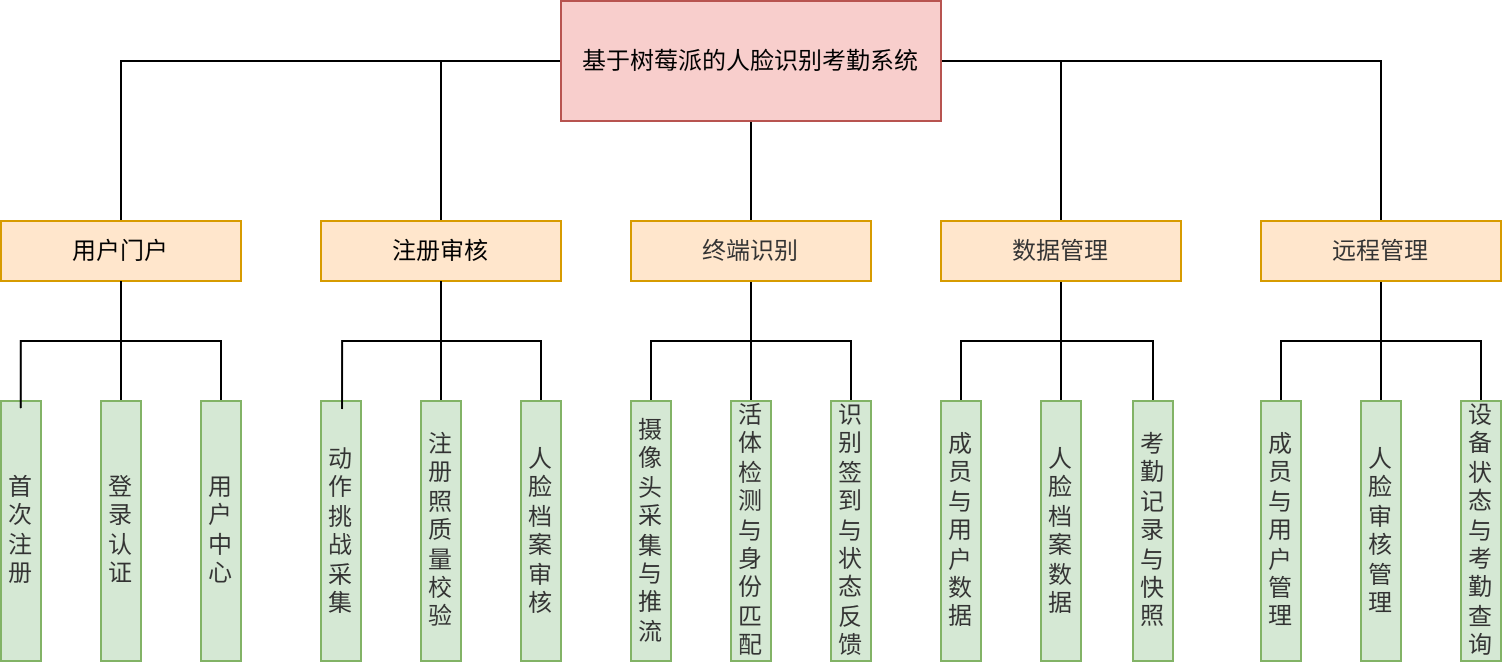
\includegraphics[width=0.86\textwidth]{figures/raspberry/image1.png}
\caption{图4.1 系统功能结构图}
\end{figure}

图4.1体现的是本系统的。用户门户负责把成员从“名单中的人员”转为“已激活的系统用户”，因此包含首次注册、登录和用户中心。注册审核负责把用户提交的现场照片转为可被终端识别的人脸档案，所以需要动作挑战、质量校验和管理员审核。终端识别只处理现场签到，不处理账号注册和审核决策，只加载已经审核通过的人脸档案并输出识别状态。数据管理将会贯穿所有模块，既保存结构化数据，也保存注册照和考勤快照路径。远程管理不直接介入摄像头线程，而是通过管理员接口读取和修改业务数据。本系统如此划分使用户、终端和管理员各自面对的功能边界比较明确。

在功能划分的基础上，系统进一步按照实际访问路径和内部处理流程组织架构。系统运行时主要面对三类入口：普通用户通过浏览器进入用户门户，完成注册、采集和状态查看；Windows管理端通过Tailscale远程访问管理员接口；终端浏览器访问识别页面和视频流，用于现场签到展示。考虑到树莓派设备算力有限，摄像头采集、模型推理、页面响应和数据库写入不能相互阻塞，因此本文将系统划分为访问入口层、业务服务层、视觉模型层以及数据与配置层，如图4.2所示。

\begin{figure}[H]
\centering
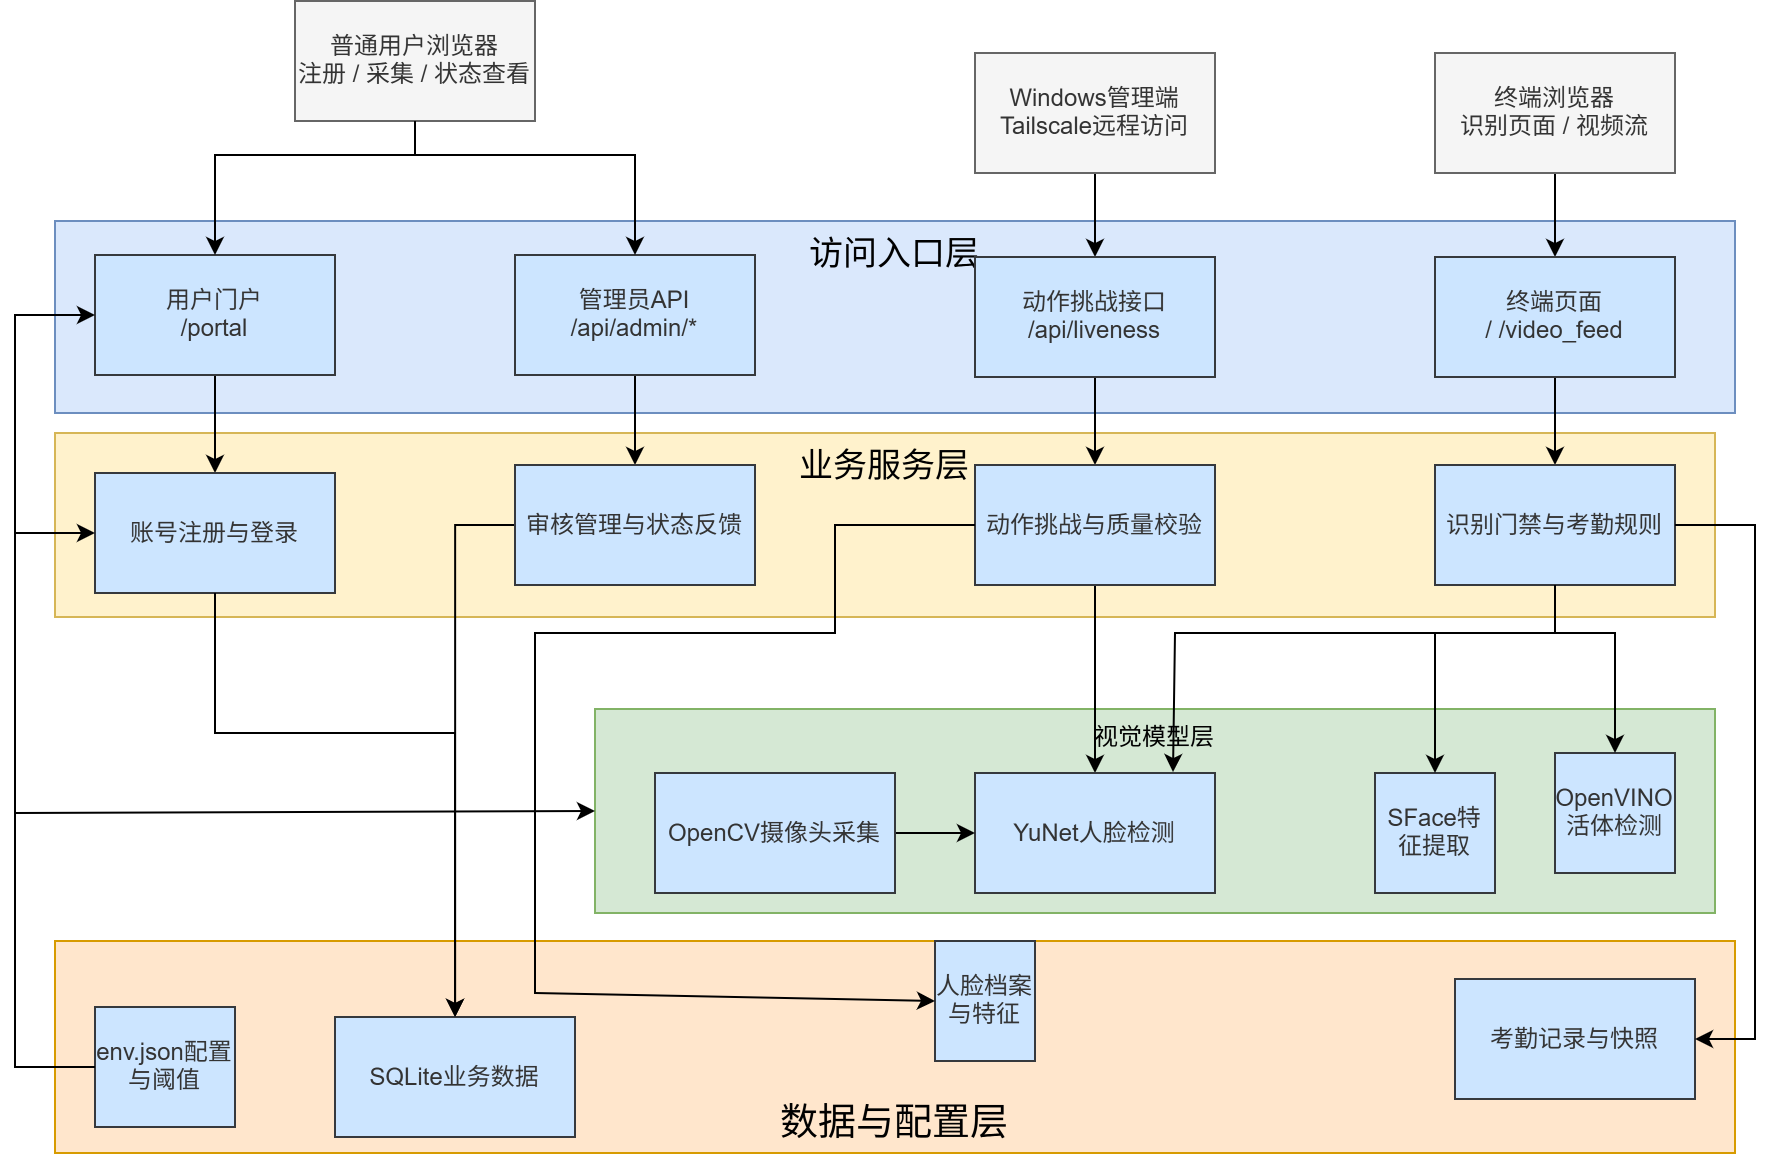
\includegraphics[width=0.86\textwidth]{figures/raspberry/image3.png}
\caption{图4.2 系统总体架构图}
\end{figure}

图4.2中，访问入口层负责接收不同使用对象的请求，包括用户门户/portal、管理员API /api/admin/*、动作挑战接口/api/liveness，以及终端页面和/video\_feed视频流。业务服务层负责把这些请求转化为具体业务处理：用户门户对应账号注册与登录，管理员API对应审核管理与状态反馈，动作挑战接口对应动作挑战与质量校验，终端页面对应识别门禁与考勤规则。视觉模型层主要承担图像采集和模型推理任务，其中OpenCV摄像头采集为YuNet人脸检测提供输入，YuNet检测结果继续供SFace特征提取和OpenVINO活体检测使用。数据与配置层保存系统运行所需的基础数据和结果数据，包括env.json配置与阈值、SQLite业务数据、人脸档案与特征、考勤记录与快照。这样组织后，用户注册、管理员审核和终端签到虽然入口不同，但最终都围绕同一套人脸档案、识别结果和考勤记录展开。

系统的部署方式如图4.3所示进行设计。树莓派端是系统的核心运行节点，连接USB摄像头并运行FastAPI服务，同时保存SQLite数据库、注册照和考勤快照。本地浏览器访问树莓派根路径进入终端识别页面；普通用户从非本地网络访问时进入用户门户；Windows管理端通过Tailscale网络调用树莓派暴露的管理员API。这样部署的好处是现场签到不依赖外部服务器，管理员又可以在不直接暴露公网端口的情况下远程完成审核和查询。

\begin{figure}[H]
\centering
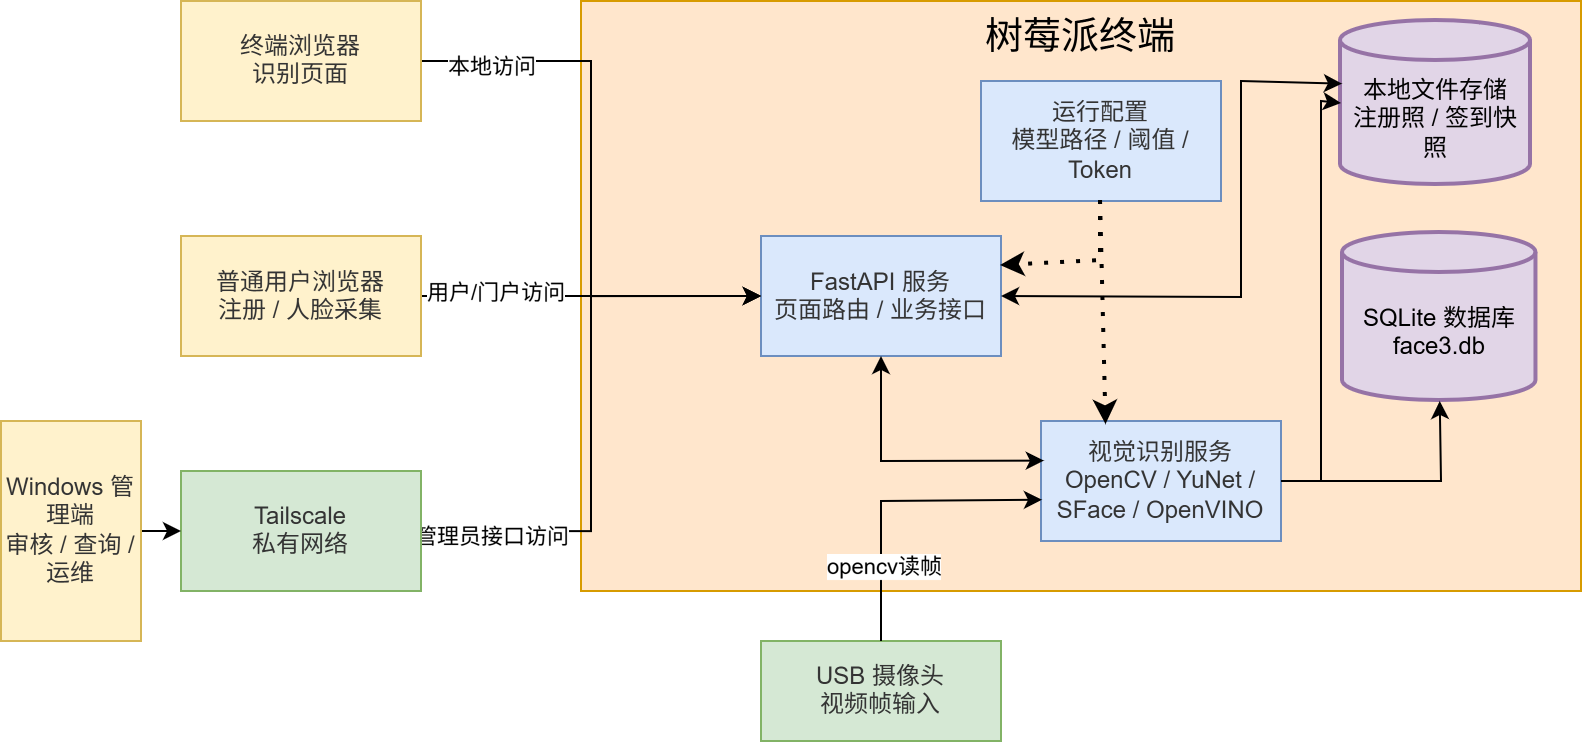
\includegraphics[width=0.86\textwidth]{figures/raspberry/image5.png}
\caption{图4.3 系统部署架构图}
\end{figure}

\section{系统核心功能设计}
\subsection{人脸注册审核}
注册审核框架主要控制进入识别库的人脸资料。对人脸考勤系统来说，入库阶段一旦出错，后续签到就很难补救。如果用户可以随意上传照片，可能出现照片模糊、多人入镜、侧脸严重、用屏幕翻拍他人照片等问题；如果系统不设置审核状态，终端又可能提前加载未经确认的人脸档案，管理员后续纠错会很麻烦。因此，本系统在注册端设计了由名单准入、账号注册、动作挑战、质量校验和管理员审核组成的入库控制模型，如图4.4所示（箭头向右为步骤成功，向下即失败）。

\begin{figure}[H]
\centering
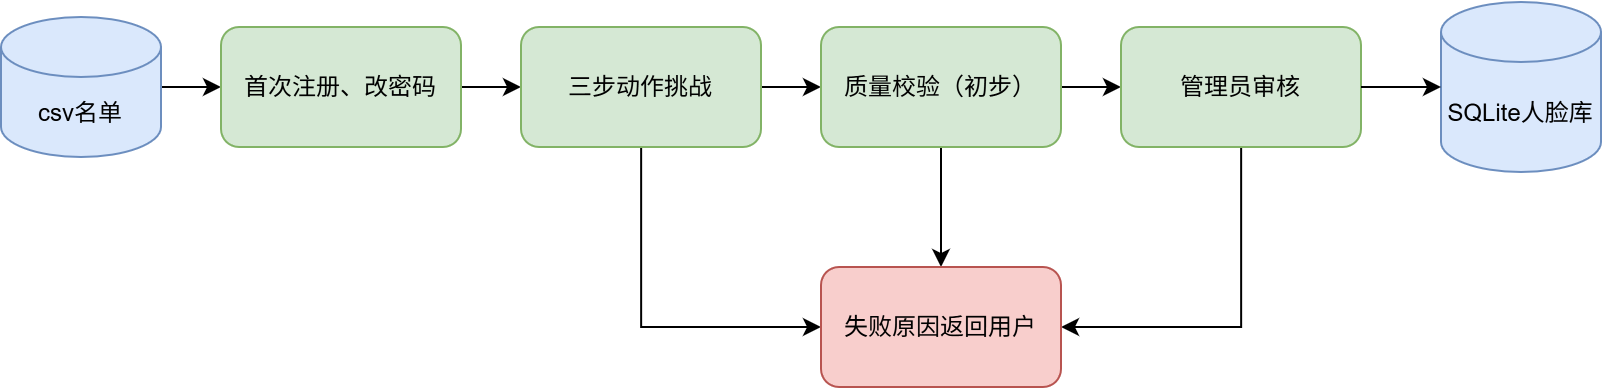
\includegraphics[width=0.86\textwidth]{figures/raspberry/image7.png}
\caption{图4.4 人脸档案审核与入库图}
\end{figure}

图4.4中的第一步是名单准入。系统通过roster\_members表保存管理员预置的成员姓名、编号、角色、状态和初始密码哈希。用户首次注册时必须输入姓名、学号或工号、初始密码、新密码和确认密码。系统先同步名单文件，再检查编号是否存在、名单状态是否为active、姓名是否与名单一致、初始密码是否正确，全部通过后才写入正式账号。也就是说，注册入口受到管理员预置名单约束，非本考勤系统内部人员的其他访问者无法绕过名单自行创建账号。

第二步是动作挑战。这一步主要是是为了增加造假的成本。动作挑战包含挑战ID、过期时间、动作步骤、已通过步骤和最终可信注册照等状态。当前动作模板为“正脸、向左或向右轻微转头、再回正脸”，其中侧转方向从预设模板中随机选择。每一步提交抓拍图后，后端都会解码图片、检测人脸、检查是否单人入镜、计算姿态指标，并与第一步通过的抓拍进行同人一致性比较。中途换人时，系统返回身份变化提示；动作幅度不符合当前步骤时，系统返回具体动作要求。三步全部通过后，系统从已通过抓拍中优先选择清晰度最高的正脸照片作为最终注册照，并在后端冻结该照片，这样就算挑战完成。正式提交时，系统便只读取最后这张可信注册照。

第三步是质量校验。动作挑战能证明用户按要求完成了现场动作，但照片能否长期用于识别还要继续检查。校验流水线先构建统一上下文，包括原始图片、BGR图、RGB图、图像尺寸、人脸框和关键点。随后依次执行单人检测、人脸面积检测、Laplacian清晰度检测、亮度均值检测、关键点完整性检测、轻量姿态检测和翻拍风险检测。每个校验器只负责一种规则，并返回统一格式的结果，包括校验名称、是否通过、错误码、中文提示、分数和阈值。这样前端可以把失败原因直接展示给用户，管理员也能根据校验项判断照片为什么没有进入审核阶段。

第四步是管理员审核。通过质量校验的照片便会提交，但是并不会立即参与终端识别，因为之前三步做的筛选并不强大健壮。且鉴于人员固定较少且上传时间有间隔，这能够决定上传人脸的流量会很低，故用最原始的方式反而最为契合本系统的人脸审核。故此照片会以pending状态写入face\_profiles表。管理员在Windows管理端查看待审核档案，可以选择通过、驳回或重新置为待审核。审核通过后，档案状态变为approved，终端识别器下次重载人脸库时才会加载该档案；审核驳回后，系统记录驳回原因、备注、审核人和审核时间，并写入驳回历史表。用户在个人中心可以看到最近人脸资料状态、审核原因和重新上传提示。这样安排后，用户可以自助提交资料，最终是否进入识别库仍由管理员确认。

\subsection{树莓派端人脸识别与活体检测}
\begin{figure}[H]
\centering
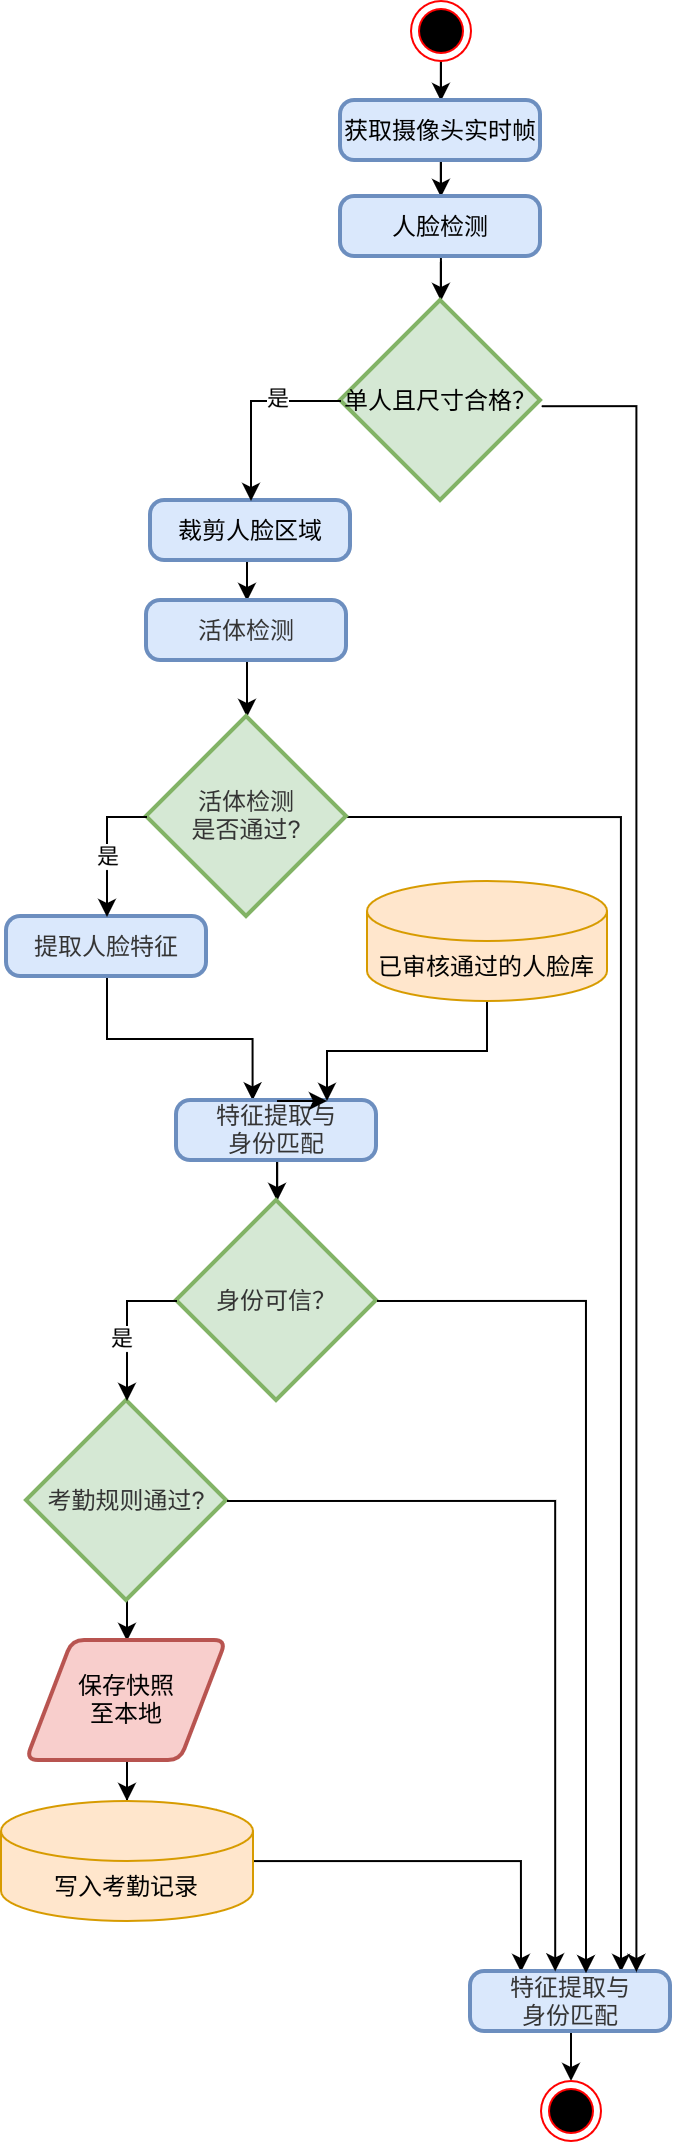
\includegraphics[width=0.86\textwidth]{figures/raspberry/image9.png}
\caption{图4.5 人脸识别与活体检测流程图}
\end{figure}

终端识别模型面向树莓派本地签到场景，输入为摄像头实时帧，输出为识别状态和考勤写入信号。系统按照“检测、活体、特征、匹配、规则”的顺序处理单帧图像。设单帧输入图像为\(I_t\)，则系统对其执行如下处理：

\begin{equation*}
R_t=A(M(L(E(D(I_t)))))\tag{4.1}
\end{equation*}

其中，\(D(\cdot)\)表示YuNet人脸检测[19,28]，\(E(\cdot)\)表示SFace特征提取[20,29]，\(L(\cdot)\)表示活体检测与重放风险判断，\(M(\cdot)\)表示身份匹配，\(A(\cdot)\)表示考勤规则判断。只有这些判断全部通过时，\(R_t\)才会被标记为可写入考勤记录。端侧识别流程如图4.5所示。

图4.5展示了终端写入考勤前的多道判断。检测到人脸只是第一步，后面还要检查人脸数量、人脸面积、活体概率、翻拍风险、身份相似度、考勤时间窗和重复签到冷却。画面中没有人脸时，终端提示用户进入画面；出现多人时暂停签到，避免身份归属不清；人脸区域过小时提示用户靠近摄像头，减少小脸裁剪导致的特征不稳定。只有这些条件都通过后，识别结果才会变为attendance\_ready。

由前文相关技术介绍可知，身份匹配采用余弦相似度。设当前帧人脸特征为\(q\)，数据库中第\(i\)个已审核人脸特征为\(k_i\)，则相似度为：

\begin{equation*}
s_i=q\cdot k_i\tag{4.2}
\end{equation*}

候选身份由最大相似度决定：

\begin{equation*}
i^*=\arg\max_i s_i\tag{4.3}
\end{equation*}

当\(s_{i^*}\geq0.363\)时，系统认为身份匹配通过。该阈值适用于本文测试时的小规模人脸库。为了降低相似样本带来的误识别风险，系统还会比较最高分和次高分之间的差距；如果两个候选身份过于接近，系统返回歧义匹配状态，要求用户重新正对摄像头。此外，终端识别还维护稳定帧计数和冷却时间。稳定帧计数用于避免瞬时匹配导致误签到；冷却时间用于避免同一用户在摄像头前停留时连续写入多条记录。

活体检测部分采用模型分数和轻量风险信号融合。单帧模型输出真人概率\(S_{\mathrm{real}}\)和伪造概率\(S_{\mathrm{spoof}}\)，但单帧分数容易受到光照、模糊和裁剪边界影响，因此系统维护2秒滑动窗口。除模型分数外，系统还计算屏幕重放风险。重放风险由频域风险、反光风险、边缘风险和矩形边框风险加权得到：

\begin{equation*}
R=0.35R_{\mathrm{freq}}+0.25R_{\mathrm{glare}}+0.15R_{\mathrm{edge}}+0.25R_{\mathrm{rect}}\tag{4.4}
\end{equation*}

其中，频域风险用于捕捉屏幕刷新或周期纹理造成的高频异常，反光风险用于描述屏幕高亮低饱和区域，边缘风险用于描述屏幕边界或纸张边缘，矩形边框风险用于判断人脸周围是否存在明显显示设备边框。最终窗口判断规则如表4.1所示。

\begingroup
\small
\begin{longtable}{|>{\raggedright\arraybackslash}p{0.307\textwidth}|>{\raggedright\arraybackslash}p{0.307\textwidth}|>{\raggedright\arraybackslash}p{0.307\textwidth}|}
\caption{表4.1 活体检测参数配置表}\\
\hline
判断项 & 当前配置 & 处理结果 \\
\hline
单帧真人阈值 & \(S_{\mathrm{real}}\geq0.55\) & 当前帧记为活体可信 \\
\hline
单帧灰区阈值 & \(0.30\leq S_{\mathrm{real}}<0.55\) & 纳入窗口，等待多帧稳定。 \\
\hline
低分累计次数 & 3次 & 达到上限后拒绝签到。 \\
\hline
窗口长度 & 2.0秒 & 统计窗口内平均真人概率和风险分数。 \\
\hline
窗口样本数 & 至少3帧 & 样本不足时提示继续保持正对摄像头。 \\
\hline
窗口真人阈值 & \(\overline{S}_{\mathrm{real}}\geq0.45\) & 作为多帧通过条件之一。 \\
\hline
重放风险阈值 & R\textless{}0.72 & 超过阈值时拒绝签到。 \\
\hline
\end{longtable}
\endgroup

表4.1 活体检测参数配置表体现了终端端和注册端的差异。注册端可以要求用户完成动作挑战，因为注册流程只发生一次，用户可以接受相对完整的采集步骤；终端端面对的是高频签到场景，显然若每次签到都要求用户做动作，会明显降低通行效率。因此终端端以被动活体检测和重放风险为主，在不增加额外操作的情况下提高照片、屏幕翻拍等攻击的识别能力。

终端识别的整体算法过程可分为三个层次：帧级处理管线、活体融合判决和重放风险分析。帧级管线是识别器对单帧图像执行的完整流程，按"预处理、检测、活体、特征、匹配、稳定、规则"的顺序逐层过滤；活体融合判决在被动活体模型输出的基础上，引入2秒滑动窗口内的多帧统计与重放风险信号，降低单帧噪声的影响；重放风险分析则从频域、反光、边缘和边框四个正交维度计算伪造概率，作为活体判决的辅助信号。算法\ref{alg:terminal}描述了帧级处理管线的完整过程，算法\ref{alg:liveness}描述了活体窗口的融合判决策略，算法\ref{alg:replay}描述了重放风险分析的计算流程。

% 恢复英文关键字（覆盖 heuthesis.cls 中的中文定义）
\makeatletter
\AtBeginDocument{%
  \algrenewcommand\algorithmicrequire{\textbf{Input:}}%
  \algrenewcommand\algorithmicensure{\textbf{Output:}}%
  \algrenewcommand\algorithmicif{\textbf{if}}%
  \algrenewcommand\algorithmicthen{\textbf{then}}%
  \algrenewcommand\algorithmicelse{\textbf{else}}%
  \algrenewcommand\algorithmicfor{\textbf{for}}%
  \algrenewcommand\algorithmicforall{\textbf{for all}}%
  \algrenewcommand\algorithmicdo{\textbf{do}}%
  \algrenewcommand\algorithmicwhile{\textbf{while}}%
  \algrenewcommand\algorithmicreturn{\textbf{return}}%
  \renewcommand{\algorithmiccomment}[1]{{\scriptsize // #1}}%
  % 定义英文 end 命令（模板的 \EndIf = "结束 if"，这里改用英文）
  \providecommand{\endIf}{\textbf{end if}}
  \providecommand{\endFor}{\textbf{end for}}
  \providecommand{\endWhile}{\textbf{end while}}
  \providecommand{\endLoop}{\textbf{end loop}}
}
\makeatother

\begin{algorithm}[htbp]
\caption{终端帧级识别管线}
\begin{algorithmic}[1]
\restoreAlgoEnglish
\Require 当前帧 $I_t$，已审核人脸库 $\mathcal{K} = \{k_1, k_2, \ldots, k_n\}$，系统配置参数
\Ensure 识别结果 $R_t$（状态码、候选身份、置信度、活体结果）

\If{$I_t$ 为空或无效}
    \State \Return 状态码: \texttt{empty\_frame}
\endIf
\If{$\mathcal{K} = \emptyset$}
    \State \Return 状态码: \texttt{no\_known\_faces}
\endIf

\Statex
\Comment{步骤1: 人脸检测}
\State $D_t \gets$ \textsc{YuNetDetect}$(I_t)$ \Comment{边界框 + 5个关键点 + 置信度}
\If{$|D_t| = 0$}
    \State \Return 状态码: \texttt{no\_face}
\ElsIf{$|D_t| > 1$}
    \State \Return 状态码: \texttt{multi\_face}
\endIf
\State $B_t \gets D_t[0]$

\Statex
\Comment{步骤2: 人脸面积校验}
\State $r_{\mathrm{face}} \gets B_t$ 的面积 $/$ $I_t$ 的面积
\If{$r_{\mathrm{face}} < r_{\min}$}
    \State \Return 状态码: \texttt{face\_too\_small}
\endIf

\Statex
\Comment{步骤3: 裁剪人脸区域并外扩边界}
\State $F_{\mathrm{roi}} \gets$ \textsc{ExtractROI}$(I_t, B_t, \text{外扩比例} = 0.08)$

\Statex
\Comment{步骤4: 被动活体检测}
\State $(S_{\mathrm{real}}, S_{\mathrm{spoof}}) \gets$ \textsc{AntiSpoofInfer}$(F_{\mathrm{roi}})$ \Comment{OpenVINO anti-spoof-mn3}
\State $R_{\mathrm{replay}} \gets$ \textsc{EstimateReplayRisk}$(I_t, F_{\mathrm{roi}}, B_t)$ \Comment{算法\ref{alg:replay}}
\State \textsc{AddLivenessSample}$(t, S_{\mathrm{real}}, R_{\mathrm{replay}})$ \Comment{加入滑动窗口}

\Statex
\Comment{步骤5: 特征提取}
\State $A_t \gets$ \textsc{AlignCrop}$(I_t, B_t)$ \Comment{利用5个关键点对齐}
\State $f_t \gets$ \textsc{SFaceFeature}$(A_t)$
\State $\hat{f}_t \gets f_t / \|f_t\|_2$

\Statex
\Comment{步骤6: 身份匹配}
\State $\mathcal{S} \gets \{s_i = \hat{f}_t \cdot k_i \mid i = 1,\ldots,n\}$ \Comment{余弦相似度}
\State $i^* \gets \arg\max_i s_i$
\State $s_{\mathrm{best}} \gets s_{i^*}$
\State $s_{\mathrm{second}} \gets$ 次高相似度值

\If{$s_{\mathrm{best}} < \tau_{\mathrm{cos}}$}
    \State \Return 状态码: \texttt{unknown}
\endIf
\If{$s_{\mathrm{second}}$ 存在 \textbf{且} $s_{\mathrm{second}} - s_{\mathrm{best}} < \delta_{\mathrm{amb}}$}
    \State \Return 状态码: \texttt{ambiguous\_match}
\endIf

\Statex
\Comment{步骤7: 多帧稳定性计数}
\State $\text{stable\_count} \gets$ \textsc{AdvanceStability}$(i^*, t)$
\If{$\text{stable\_count} < N_{\mathrm{stable}}$}
    \State \Return 状态码: \texttt{match\_not\_stable\_yet}
\endIf

\Statex
\Comment{步骤8: 活体窗口判决}
\State $W_t \gets$ \textsc{GetLivenessWindow}$(t)$
\State $l_{\mathrm{result}} \gets$ \textsc{EvaluatePassiveLiveness}$(W_t)$ \Comment{算法\ref{alg:liveness}}
\If{$l_{\mathrm{result}} = \texttt{spoof\_suspected}$}
    \State 重置识别跟踪状态
    \State \Return 状态码: \texttt{spoof\_suspected}
\ElsIf{$l_{\mathrm{result}} = \texttt{liveness\_uncertain}$}
    \State \Return 状态码: \texttt{liveness\_uncertain}
\endIf

\Statex
\Comment{步骤9: 考勤规则校验}
\If{$t \notin [T_{\mathrm{start}}, T_{\mathrm{end}}]$}
    \State \Return 状态码: \texttt{outside\_attendance\_window}
\endIf
\State $\Delta_{\mathrm{cooldown}} \gets$ \textsc{CooldownRemaining}$(\text{user}_{i^*}, t)$
\If{$\Delta_{\mathrm{cooldown}} > 0$}
    \State \Return 状态码: \texttt{attendance\_cooldown}
\endIf

\Statex
\Comment{步骤10: 可选的动作挑战活体确认}
\If{\textsc{ShouldRequireChallenge}$(S_{\mathrm{real}}, \text{stable\_count}, s_{\mathrm{best}}, t)$}
    \State $c_{\mathrm{result}} \gets$ \textsc{AdvanceChallenge}$(I_t, B_t, \text{user}_{i^*}, t)$
    \If{$c_{\mathrm{result}} \neq \text{None}$}
        \State \Return 状态码: $c_{\mathrm{result}}$
    \endIf
\endIf

\Statex
\Comment{步骤11: 签到就绪}
\State \Return 状态码: \texttt{attendance\_ready}, 身份: $i^*$, 置信度: $\text{Confidence}(s_{\mathrm{best}})$
\end{algorithmic}
\label{alg:terminal}
\end{algorithm}

\begin{algorithm}[htbp]
\caption{被动活体窗口融合判决}
\begin{algorithmic}[1]
\Require 滑动窗口样本集 $W = \{w_1, w_2, \ldots, w_m\}$，其中 $w_j = (S_{\mathrm{real}}^{(j)}, R_{\mathrm{replay}}^{(j)}, \text{checked}_j)$
\Ensure 活体判决结果：\texttt{None}（通过）、\texttt{spoof\_suspected}、\texttt{liveness\_uncertain}

\State $M \gets |\{w_j \in W \mid \text{checked}_j = \text{True}\}|$ \Comment{有效检测样本数}
\If{$M = 0$}
    \State \Return \texttt{None} \Comment{活体检测未启用或不可用，放行}
\endIf
\If{$M < M_{\min}$}
    \State \Return \texttt{liveness\_uncertain}
\endIf

\Statex
\Comment{统计窗口内指标}
\State $\overline{S}_{\mathrm{real}} \gets \frac{1}{M} \sum\limits_{j=1}^{M} S_{\mathrm{real}}^{(j)}$
\State $R_{\max} \gets \max\limits_{j} R_{\mathrm{replay}}^{(j)}$
\State $C_{\mathrm{low}} \gets |\{w_j \in W \mid S_{\mathrm{real}}^{(j)} < \tau_{\mathrm{gray}}\}|$ \Comment{低分样本数}

\Statex
\Comment{多重拒绝条件}
\If{$C_{\mathrm{low}} \geq C_{\mathrm{fail}}$}
    \State \Return \texttt{spoof\_suspected}
\ElsIf{$R_{\max} \geq \tau_{\mathrm{replay}}$}
    \State \Return \texttt{spoof\_suspected}
\ElsIf{$\overline{S}_{\mathrm{real}} < \tau_{\mathrm{uncertain}}^{\mathrm{real}}$ \textbf{且} $\frac{1}{M} \sum\limits_j R_{\mathrm{replay}}^{(j)} \geq \tau_{\mathrm{uncertain}}^{\mathrm{replay}}$}
    \State \Return \texttt{spoof\_suspected}
\ElsIf{$\overline{S}_{\mathrm{real}} < \tau_{\mathrm{window}}^{\mathrm{real}}$}
    \State \Return \texttt{liveness\_uncertain}
\ElsIf{$\frac{1}{M} \sum\limits_j R_{\mathrm{replay}}^{(j)} \geq \tau_{\mathrm{uncertain}}^{\mathrm{replay}}$}
    \State \Return \texttt{liveness\_uncertain}
\endIf
\State \Return \texttt{None}
\end{algorithmic}
\label{alg:liveness}
\end{algorithm}

\begin{algorithm}[htbp]
\caption{屏幕重放风险分析}
\begin{algorithmic}[1]
\Require 当前帧 $I_t$，裁剪人脸区域 $F_{\mathrm{roi}}$，人脸边界框 $B_t$
\Ensure 重放风险评分 $R_{\mathrm{replay}} \in [0, 1]$

\State $G \gets$ \textsc{GrayScale}($F_{\mathrm{roi}}$ 缩放到 $96 \times 96$)

\Statex
\Comment{1. 反光风险（25\%）}
\State $H \gets$ \textsc{HSV}($F_{\mathrm{roi}}$ 缩放到 $96 \times 96$)
\State $\text{glare\_ratio} \gets \frac{1}{|H|} |\{(v, s) \in H \mid v > 245 \text{ 且 } s < 70\}|$
\State $R_{\mathrm{glare}} \gets \text{clamp}_{[0,1]}\left(\frac{\text{glare\_ratio} - 0.02}{0.10}\right)$

\Statex
\Comment{2. 边缘风险（15\%）}
\State $E \gets$ \textsc{Canny}$(G, 80, 160)$
\State $\text{edge\_density} \gets \frac{1}{|G|} |E|$
\State $R_{\mathrm{edge}} \gets \text{clamp}_{[0,1]}\left(\frac{\text{edge\_density} - 0.18}{0.20}\right)$

\Statex
\Comment{3. 摩尔纹风险（35\%）}
\State $\tilde{G} \gets G - \text{mean}(G)$
\State $\mathcal{F} \gets \text{fftshift}(\text{fft2}(\tilde{G}))$
\State $\mathcal{M} \gets |\mathcal{F}|$
\State $\text{high\_freq} \gets \sum\limits_{(u,v): \rho(u,v) \geq 0.45} \mathcal{M}(u,v)$，其中 $\rho(u,v)$ 为归一化径向距离
\State $\text{total\_freq} \gets \sum\limits_{u,v} \mathcal{M}(u,v) + \epsilon$
\State $\text{hf\_ratio} \gets \text{high\_freq} / \text{total\_freq}$
\State $R_{\mathrm{freq}} \gets \text{clamp}_{[0,1]}\left(\frac{\text{hf\_ratio} - 0.36}{0.22}\right)$

\Statex
\Comment{4. 矩形边框风险（25\%）}
\State $R_{\mathrm{rect}} \gets 0$
\State $E_{\mathrm{full}} \gets$ \textsc{Canny}(\textsc{GaussianBlur}($I_t$ 灰度), $60, 160$)
\ForAll{轮廓 $C$ \textbf{in} $E_{\mathrm{full}}$}
    \If{$\text{Area}(C) < 0.035 \times \text{Area}(I_t)$}
        \State 继续下一个轮廓
    \endIf
    \State $P \gets$ \textsc{ApproxPoly}$(C, 0.03 \times \text{Perimeter}(C))$
    \If{$4 \leq |P| \leq 6$ \textbf{且} \textsc{EnclosesFace}$(C, B_t)$ \textbf{且} \textsc{Rectangularity}$(C) \geq 0.70$}
        \State $R_{\mathrm{rect}} \gets 1.0$
        \State 跳出循环
    \endIf
\endFor

\Statex
\Comment{加权合成}
\State $R_{\mathrm{replay}} \gets \text{clamp}_{[0,1]}(0.35 R_{\mathrm{freq}} + 0.25 R_{\mathrm{glare}} + 0.15 R_{\mathrm{edge}} + 0.25 R_{\mathrm{rect}})$
\State \Return $R_{\mathrm{replay}}$
\end{algorithmic}
\label{alg:replay}
\end{algorithm}

\section{数据库与接口协同设计}
系统采用SQLite数据库[24]保存成员、用户、人脸档案、驳回历史和考勤记录。。成员名单表表示“允许进入系统的人”；用户表表示“已经完成首次注册的人”；人脸档案表表示“用户提交过的人脸资料及审核状态”；驳回历史表表示“管理员为什么拒绝某次资料”；考勤记录表表示“某人在某时完成过一次签到”。这些表之间的关系如图4.6所示。

\begin{figure}[H]
\centering
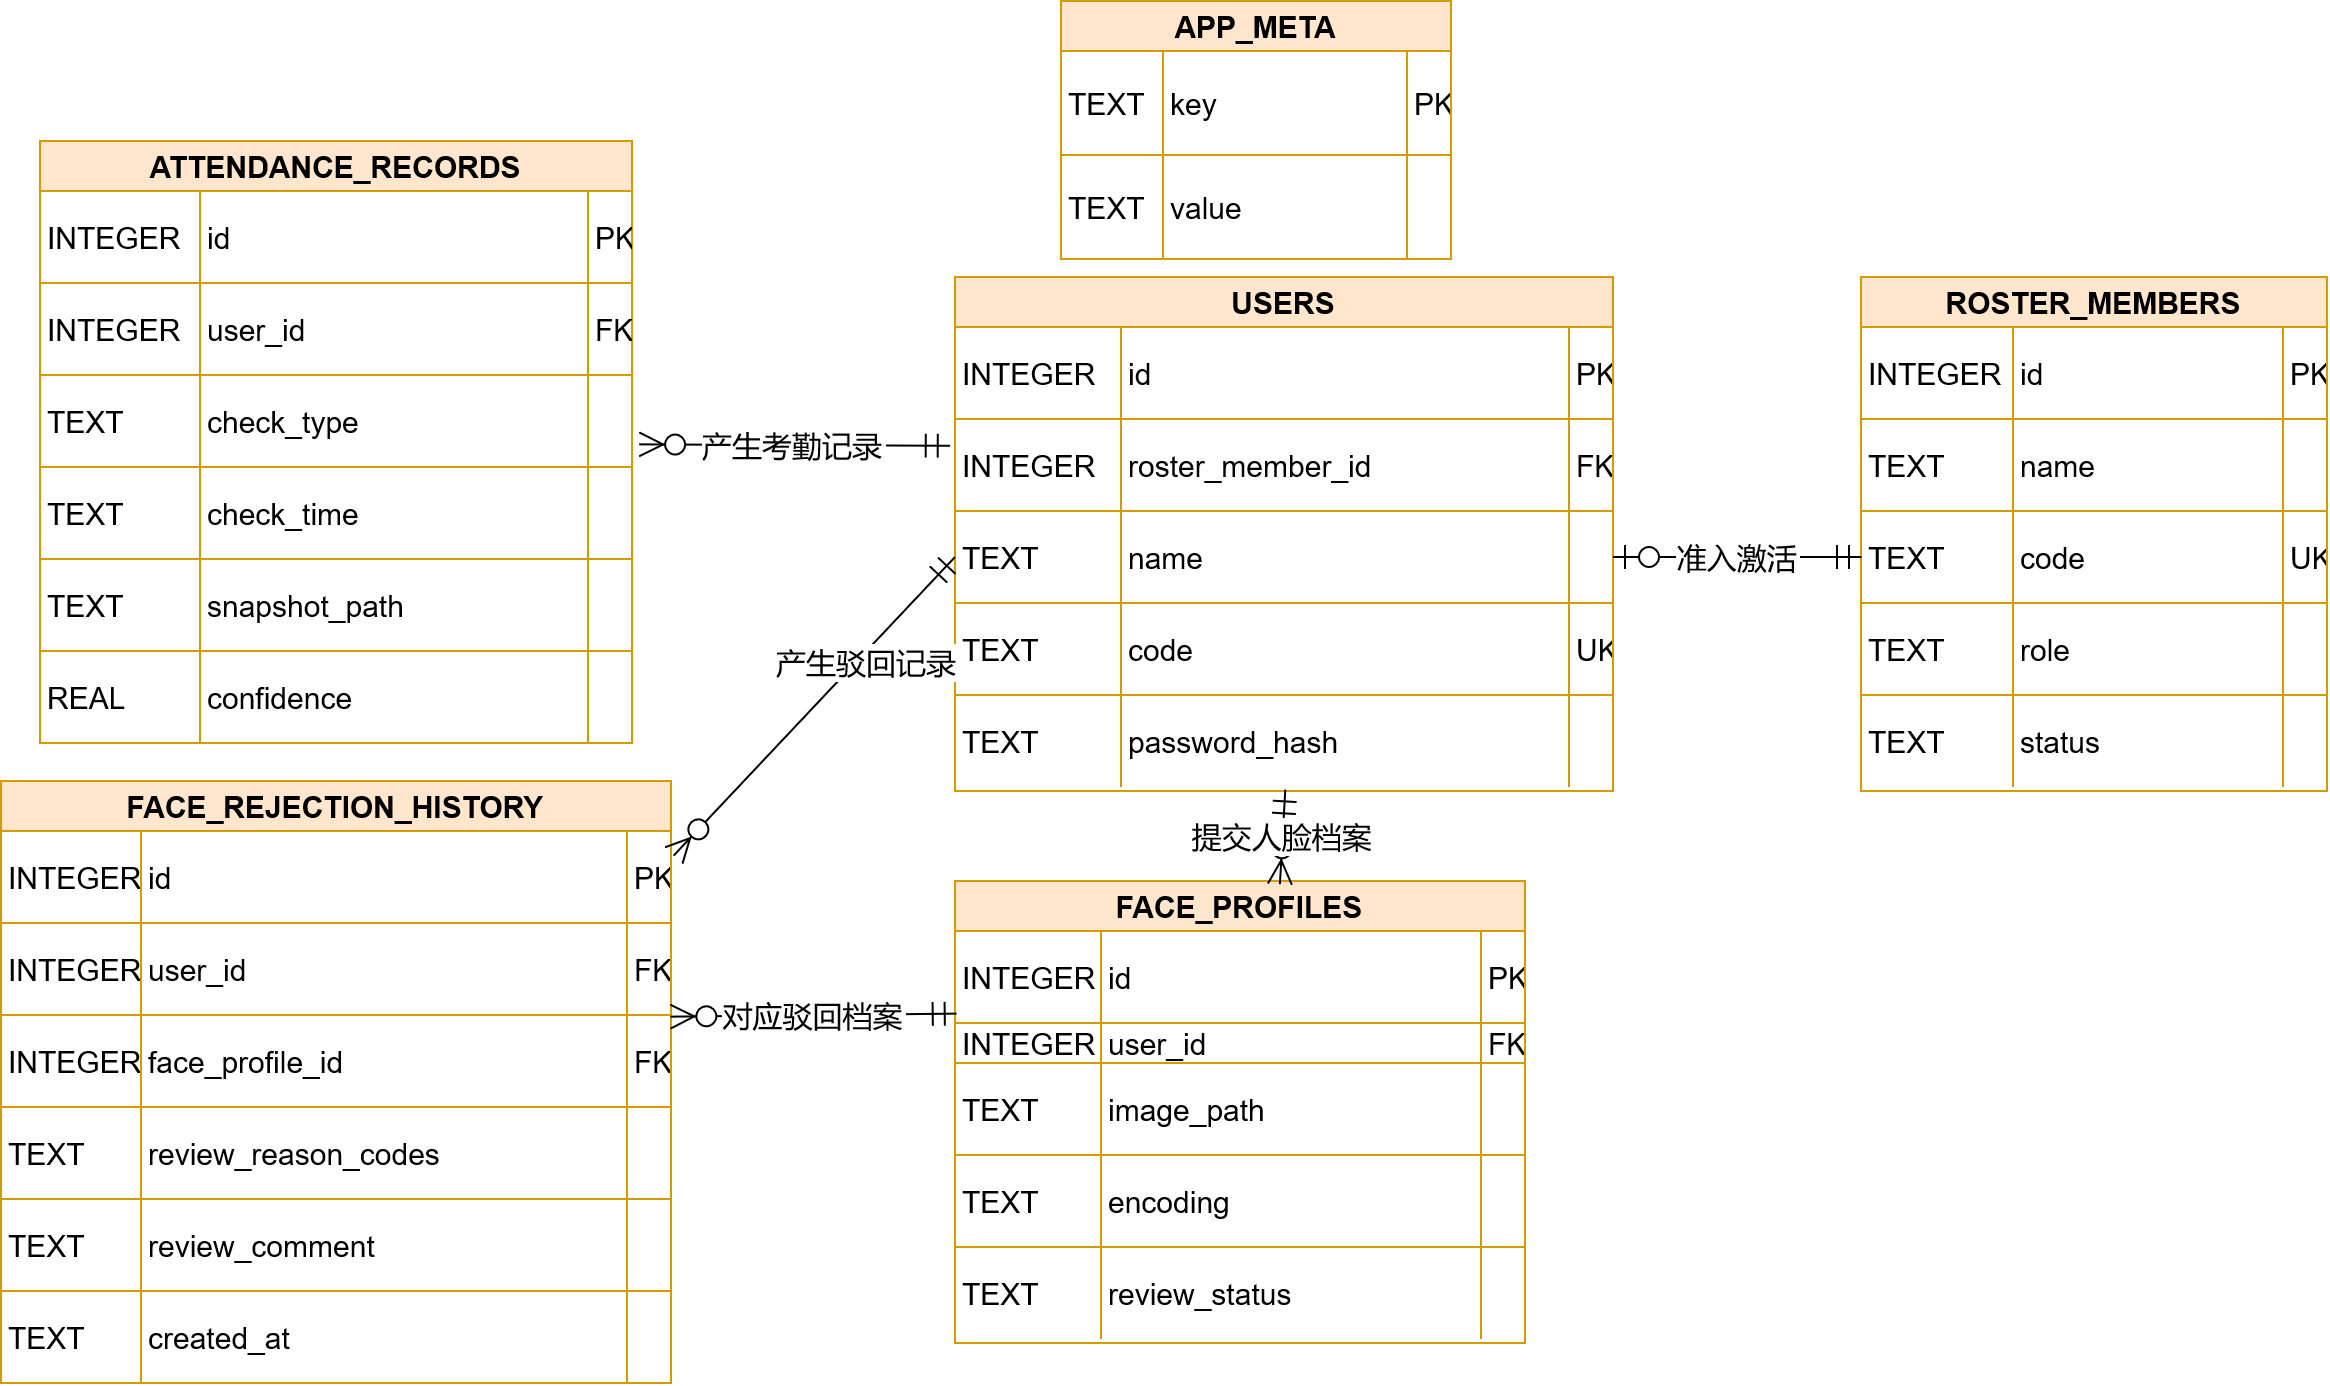
\includegraphics[width=0.86\textwidth]{figures/raspberry/image11.png}
\caption{图4.6 核心数据表实体关系图}
\end{figure}

图4.6中，成员名单是用户注册的准入来源，用户表是人脸档案和考勤记录的中心实体，人脸档案审核状态决定终端是否加载该档案。一个成员名单记录最多激活为一个用户账号，一个用户可以产生人脸档案和考勤记录，驳回历史同时关联用户和被驳回的人脸档案。应用元数据表不直接参与业务查询，主要记录轻量迁移状态，避免某些只应执行一次的历史数据处理被重复执行。核心表结构如表4.2所示。

\begingroup
\small
\begin{longtable}{|>{\raggedright\arraybackslash}p{0.307\textwidth}|>{\raggedright\arraybackslash}p{0.307\textwidth}|>{\raggedright\arraybackslash}p{0.307\textwidth}|}
\caption{表4.2 核心数据表的说明}\\
\hline
数据表 & 字段 & 设计说明 \\
\hline
roster\_members & id,name,code,role,status,initial\_password\_hash,created\_at,updated\_at & 成员白名单表。code唯一，status控制成员是否允许继续使用系统，初始密码以哈希形式保存 \\
\hline
users & id,roster\_member\_id,name,code,password\_hash,password\_changed\_at, last\_login\_at,created\_at & 用户账号表。与成员名单通过roster\_member\_id关联，password\_hash为空表示尚未完成首次注册 \\
\hline
\end{longtable}
\endgroup

\begingroup
\small
\begin{longtable}{|>{\raggedright\arraybackslash}p{0.307\textwidth}|>{\raggedright\arraybackslash}p{0.307\textwidth}|>{\raggedright\arraybackslash}p{0.307\textwidth}|}
\caption{(续)表4.2}\\
\hline
数据表 & 字段 & 设计说明 \\
\hline
face\_profiles & id,user\_id,image\_path,encoding,review\_status,review\_reason\_codes,review\_comment,reviewed\_at, reviewed\_by,created\_at & 人脸档案表。保存注册照路径、特征向量和审核状态。review\_status取pending、approved、rejected \\
\hline
face\_rejection\_history & id,user\_id,face\_profile\_id,review\_reason\_codes,review\_comment,reviewed\_by,created\_at & 驳回历史表。记录近几次驳回原因，供用户中心和管理员端追溯 \\
\hline
attendance\_records & id,user\_id,check\_type,check\_time,snapshot\_path,confidence & 考勤记录表。保存签到类型、签到时间、现场快照路径和识别置信度 \\
\hline
app\_meta & key,value & 应用元数据表。用于记录轻量迁移状态，避免重复执行时间修正等迁移逻辑 \\
\hline
\end{longtable}
\endgroup

表4.2中的字段设计与系统流程相对应。成员名单表中的编号唯一约束用于避免同一学号或工号重复出现；用户表中的正式密码哈希和最近登录时间用于区分“名单存在但未注册”和“已经完成注册”；人脸档案表中的review\_status是终端识别库加载的关键条件，只有approved档案会进入识别；驳回历史表保存原因码和备注，方便用户根据反馈重新拍摄；考勤记录表保存现场快照路径和识别置信度，便于管理员事后核查。系统还为成员状态、人脸档案用户ID、人脸审核状态、考勤用户ID、考勤时间和驳回历史用户ID建立索引，以支持管理员端按状态、日期、姓名和编号进行查询。

接口设计与数据库设计保持一致，按访问对象分为用户门户接口、动作挑战接口、本地终端接口和管理员接口。用户门户接口依赖浏览器Session，适合普通用户登录后查看和提交自己的资料；本地终端接口只面向树莓派本地浏览器，主要提供视频流和识别状态；管理员接口面向Windows管理端，必须携带Token。接口分组如表4.3所示

\begingroup
\small
\begin{longtable}{|>{\raggedright\arraybackslash}p{0.230\textwidth}|>{\raggedright\arraybackslash}p{0.230\textwidth}|>{\raggedright\arraybackslash}p{0.230\textwidth}|>{\raggedright\arraybackslash}p{0.230\textwidth}|}
\caption{表4.3 接口分组设计}\\
\hline
接口类别 & 典型路径 & 鉴权方式 & 主要功能 \\
\hline
用户门户 & /portal/*，/api/portal/* & Session 会话 & 首次注册、登录、用户中心、人脸资料提交、审核状态查看 \\
\hline
\end{longtable}
\endgroup

\begingroup
\small
\begin{longtable}{|>{\raggedright\arraybackslash}p{0.230\textwidth}|>{\raggedright\arraybackslash}p{0.230\textwidth}|>{\raggedright\arraybackslash}p{0.230\textwidth}|>{\raggedright\arraybackslash}p{0.230\textwidth}|}
\caption{(续)表4.3}\\
\hline
接口类别 & 典型路径 & 鉴权方式 & 主要功能 \\
\hline
动作挑战 & /api/liveness/* & Session会话 & 创建挑战、提交每一步抓拍、返回姿态与同人校验结果 \\
\hline
本地终端 & /，/video\_feed，/api/terminal/* & 本地访问策略 & 展示实时视频流、识别进度、今日概况和现场公告 \\
\hline
管理员接口 & /api/admin/* & Bearer Token & 设备状态、成员管理、用户管理、人脸审核、考勤查询、快照访问 \\
\hline
\end{longtable}
\endgroup

管理员接口是Windows端和树莓派端之间的主要通信边界，其设计既要覆盖管理功能，也要避免Windows端越过HTTP边界直接操作树莓派文件系统。管理员接口细化如表4.4所示。

\begingroup
\small
\begin{longtable}{|>{\raggedright\arraybackslash}p{0.307\textwidth}|>{\raggedright\arraybackslash}p{0.307\textwidth}|>{\raggedright\arraybackslash}p{0.307\textwidth}|}
\caption{表4.4 管理员接口细化}\\
\hline
接口组 & 对应接口 & 说明 \\
\hline
设备状态 & GET /device/info；GET /device/health；GET /device/metrics；POST /device/reload-config & 查询设备身份、运行状态、数据库状态、摄像头状态、资源指标，并支持重新加载配置 \\
\hline
成员名单 & GET /roster-members；POST /roster-members/sync；POST /roster-members；PUT /roster-members/\{id\} & 同步CSV名单，查询、新增和更新成员。成员编号用于约束首次注册 \\
\hline
用户管理 & GET /users；GET /users/\{id\}；POST /users/\{id\}/status；POST /users/\{id\}/password/reset & 查看用户注册状态、人脸档案统计，支持停用成员和重置正式密码 \\
\hline
人员档案 & GET /face-profiles；GET /face-profiles/\{id\}；GET /face-profiles/\{id\}/image；POST /face-profiles/\{id\}/review；DELETE /face-profiles/\{id\} & 查询待审核、已通过、已驳回人脸档案，查看图片并提交审核结果 \\
\hline
\end{longtable}
\endgroup

\begingroup
\small
\begin{longtable}{|>{\raggedright\arraybackslash}p{0.307\textwidth}|>{\raggedright\arraybackslash}p{0.307\textwidth}|>{\raggedright\arraybackslash}p{0.307\textwidth}|}
\caption{(续)表4.4}\\
\hline
接口组 & 对应接口 & 说明 \\
\hline
考勤记录 & GET /attendance；GET /attendance/today-summary；GET /attendance/\{id\}/snapshot & 按日期、姓名、编号查询考勤，获取今日汇总，查看签到快照 \\
\hline
\end{longtable}
\endgroup

系统的访问边界按照角色和来源划分。本地环回地址用于终端页、视频流和终端接口；普通远程访问进入用户门户；管理员API作为独立入口，只接受携带Authorization Bearer Token或X-Admin-Token的请求。人脸图片和签到快照不直接放成公开静态资源，普通用户只能通过会话查看本人资料，管理员也需要经过鉴权接口读取图片或快照。这样处理后，用户自助注册、现场签到和远程审核可以共用同一台树莓派服务，同时减少不同角色之间的越权访问机会。

\chapter{系统功能实现与测试分析}
第五章按照实际落地顺序说明系统实现。首先给出树莓派端和Windows管理端的运行环境，然后说明配置加载、SQLite初始化和本地文件持久化方式，接着展开用户门户、注册采集、终端识别、管理员接口和测试结果。树莓派端负责现场采集、推理和写库，Windows端通过Tailscale访问管理员接口，两端之间主要通过HTTP接口协作。

\section{系统运行环境与配置}

\subsection{树莓派硬件与系统环境}
\begingroup
\small
\begin{longtable}{|>{\raggedright\arraybackslash}p{0.307\textwidth}|>{\raggedright\arraybackslash}p{0.307\textwidth}|>{\raggedright\arraybackslash}p{0.307\textwidth}|}
\caption{表5.1 树莓派硬件与系统环境}\\
\hline
类别 & 配置 & 说明 \\
\hline
终端设备 & Raspberry Pi 3b+，1GB（906MB）内存，2048MB交换区 & 作为边缘考勤终端，负责采集、识别和本地存储 \\
\hline
操作系统 & Raspberry Pi OS 64位 & 提供Linux运行环境、USB摄像头访问和网络服务能力 \\
\hline
Python版本 & 3.9 & 说明版本，确保兼容性 \\
\hline
摄像头 & 普通USB摄像头 & 通过OpenCV读取图像帧，用于终端签到和注册抓拍 \\
\hline
服务端口 & 5000 & FastAPI服务监听端口，终端页面、用户门户和管理员API共用该服务 \\
\hline
网络方式 & 局域网/Tailscale & 本地通过ssh访问树莓派，Windows管理端通过Tailnet访问管理员API \\
\hline
数据库 & SQLite & 保存名单、用户、人脸档案、审核历史和考勤记录 \\
\hline
\end{longtable}
\endgroup

树莓派硬件与系统环境如上表5.1所示。

表5.1中的配置体现了本文系统的边缘部署特点。树莓派不仅要做一个摄像头采集设备，还要承担后端服务、视觉推理和数据持久化的工作。SQLite以单文件形式保存数据，比较适合本课题这种小规模场景；FastAPI可以同时提供页面路由、JSON接口和流式响应，而且其技术较新越发成为主流框架；端口统一为5000后，本地终端、用户门户和Windows管理端都能使用同一服务入口。实际部署时，树莓派端只要完成Python环境、模型文件、数据库目录和摄像头权限配置，就可以独立运行。

\subsection{树莓派后端配置}
\begingroup
\small
\begin{longtable}{|>{\raggedright\arraybackslash}p{0.307\textwidth}|>{\raggedright\arraybackslash}p{0.307\textwidth}|>{\raggedright\arraybackslash}p{0.307\textwidth}|}
\caption{表5.2 树莓派后端主要依赖}\\
\hline
依赖 & 版本 & 用途 \\
\hline
FastAPI & 0.128.8 & 提供页面路由、JSON接口、管理员API和请求处理 \\
\hline
Starlette & 0.49.3 & FastAPI底层ASGI能力，提供Session中间件、静态文件和响应对象 \\
\hline
Uvicorn & 0.39.0 & ASGI服务器，负责运行FastAPI应用 \\
\hline
Jinja2 & 3.1.6 & 渲染终端页、登录页、注册页和用户中心模板 \\
\hline
OpenCV-Python & 4.13.0.92 & 摄像头读帧、图像处理、MJPEG编码和基础视觉算法 \\
\hline
OpenCV-Contrib-Python & 4.13.0.92 & 提供YuNet与SFace所需的人脸检测和识别接口 \\
\hline
OpenVINO & 2024.6.0 & 加载anti-spoof-mn3模型，完成CPU端被动活体推理 \\
\hline
NumPy & 1.26.4 & 图像矩阵、特征向量和相似度计算 \\
\hline
Pillow & 11.3.0 & 图像文件处理和部分图片格式兼容 \\
\hline
Pydantic & 2.13.0 & FastAPI请求与响应数据结构校验 \\
\hline
itsdangerous & 2.2.0 & 支持Session签名相关能力 \\
\hline
\end{longtable}
\endgroup

树莓派后端主要依赖如上表5.2所示。表中列出了系统运行环境中使用的主要软件包及其版本。

\subsection{树莓派前端配置}
树莓派前端页面没有引入复杂构建工具（例如很多系统流行使用vue+vite），主要采用Jinja2模板、Bootstrap样式和原生JavaScript。这样处理是考虑到系统页面数量有限，功能以表单、状态展示、摄像头预览和接口轮询为主。使用服务端模板可以减少额外打包步骤，也便于后端直接注入用户状态、审核状态和设备信息。

前端页面环境如表5.3所示。

\begingroup
\small
\begin{longtable}{|>{\raggedright\arraybackslash}p{0.307\textwidth}|>{\raggedright\arraybackslash}p{0.307\textwidth}|>{\raggedright\arraybackslash}p{0.307\textwidth}|}
\caption{表5.3 树莓派前端页面环境}\\
\hline
组成 & 版本或来源 & 用途 \\
\hline
Jinja2模板 & 3.1.6 & 负责页面结构复用和服务端变量注入 \\
\hline
Bootstrap样式 & 页面静态资源引入 & 提供表单、按钮、栅格和响应式基础样式 \\
\hline
Bootstrap Icons & 页面静态资源引入 & 提供终端页和门户页中的图标元素 \\
\hline
原生JavaScript & 浏览器内置 & 完成注册表单提交、动作挑战抓拍、终端状态轮询和页面局部刷新 \\
\hline
MJPEG视频流 & FastAPI StreamingResponse & 终端页面通过/video\_feed展示实时摄像头画面。 \\
\hline
\end{longtable}
\endgroup

\subsection{Windows管理端配置}
Windows管理端是独立于树莓派终端的管理后台。它的主要工作通过Tailscale网络请求树莓派的/api/admin/*接口，进而获取树莓派设备的实时信息、系统数据以及对系统数据进行操作。下表5.4展示了windows端的环境配置。

\begingroup
\small
\begin{longtable}{|>{\raggedright\arraybackslash}p{0.307\textwidth}|>{\raggedright\arraybackslash}p{0.307\textwidth}|>{\raggedright\arraybackslash}p{0.307\textwidth}|}
\caption{表5.4 Windows 管理端环境}\\
\hline
组成 & 版本 & 用途 \\
\hline
Python & 3.9 & 与树莓派端保持一致，降低跨端脚本和模型处理差异。 \\
\hline
uv & 0.11.3 & 管理 Windows 端依赖和虚拟环境，减少手工安装差异。 \\
\hline
\end{longtable}
\endgroup

\begingroup
\small
\begin{longtable}{|>{\raggedright\arraybackslash}p{0.307\textwidth}|>{\raggedright\arraybackslash}p{0.307\textwidth}|>{\raggedright\arraybackslash}p{0.307\textwidth}|}
\caption{(续)表5.4}\\
\hline
组成 & 版本 & 用途 \\
\hline
FastAPI & 0.128.8 & 提供Windows本地管理后台页面路由和代理接口 \\
\hline
Uvicorn & 0.39.0 & 运行Windows本地管理后台服务 \\
\hline
Jinja2 & 3.1.6 & 渲染仪表盘、成员、人脸审核和考勤页面 \\
\hline
httpx & 0.28.1 & 封装Windows端到树莓派管理员API的HTTP请求 \\
\hline
Pydantic / pydantic-settings & 2.13.2/2.11.0 & 校验远端返回结构，并读取Windows端环境变量 \\
\hline
Tailscale & 能运行即可 & 建立Windows电脑与树莓派之间的私有网络访问通道 \\
\hline
\end{longtable}
\endgroup

\section{配置管理与本地持久化实现}
系统配置由默认配置和env.json共同组成。程序启动时先读取默认配置，再用env.json中的配置项覆盖默认值。配置对象支持属性式访问和字典式访问，并在访问时检查配置文件修改时间；如果文件发生变化，系统会重新加载配置。摄像头分辨率、识别帧率、模型路径、相似度阈值、活体阈值、考勤时间段、设备名称、管理员Token等参数都集中在配置中维护。当前运行配置中，终端摄像头宽度为1280，高度为720，摄像头帧率为15FPS，识别目标帧率为5FPS；人脸检测使用YuNet，人脸特征提取使用SFace，余弦相似度阈值为0.363；活体检测启用，推理设备为CPU；考勤规则采用间隔限制模式，重复签到阻塞时间为60秒，签到快照保留7天。关键运行配置如表5.5所示。

\begingroup
\small
\begin{longtable}{|>{\raggedright\arraybackslash}p{0.307\textwidth}|>{\raggedright\arraybackslash}p{0.307\textwidth}|>{\raggedright\arraybackslash}p{0.307\textwidth}|}
\caption{表5.5 系统关键运行配置参数}\\
\hline
配置项 & 当前值 & 作用 \\
\hline
camera\_width/camera\_height & 1280/720 & 控制终端摄像头采集分辨率 \\
\hline
camera\_fps & 15 & 控制采集线程目标帧率 \\
\hline
recognition\_target\_fps & 5 & 控制识别线程处理频率，避免CPU长时间满载 \\
\hline
\end{longtable}
\endgroup

\begingroup
\small
\begin{longtable}{|>{\raggedright\arraybackslash}p{0.307\textwidth}|>{\raggedright\arraybackslash}p{0.307\textwidth}|>{\raggedright\arraybackslash}p{0.307\textwidth}|}
\caption{(续)表5.5}\\
\hline
配置项 & 当前值 & 作用 \\
\hline
face\_sface\_cosine\_threshold & 0.363 & 控制SFace余弦相似度匹配阈值 \\
\hline
attendance\_liveness\_enabled & true & 控制终端是否启用被动活体检测 \\
\hline
attendance\_liveness\_real\_threshold & 0.55 & 控制单帧真人概率通过阈值 \\
\hline
attendance\_duplicate\_block\_seconds & 60（秒） & 控制同一用户重复签到冷却时间 \\
\hline
attendance\_snapshot\_retention\_days & 7 & 控制本地签到快照保留天数 \\
\hline
\end{longtable}
\endgroup

数据库初始化由SQLite底座模块（负责确保系统运行时所有数据准确无误）完成。系统启动时执行建表语句，有则不作为，无则建立对应的表。其中，对于已经存在的数据库，系统不会删除重建，而是通过字段检查补齐新增列。例如，某次开发中对用户表增加了passwordhash这一字段，那么这次系统启动便会自动补上这一字段。本文项目的数据结构并不复杂，但开发过程中字段确实有过调整，因此采用这种轻量迁移方式可以避免破坏已有名单、用户和考勤记录。系统还使用app\_meta表记录迁移状态，对于只应执行一次的历史时间修正，先检查元数据表标记，确认尚未执行后再运行。

业务层不直接拼接数据库连接，而是通过Repository封装常用操作。Repository内部使用上下文管理器管理事务，正常执行结束后提交，出现异常时回滚并关闭连接。成员导入、用户注册、人脸档案审核和考勤写入都通过Repository完成。这样可以减少路由层和业务服务中的重复代码，也能让相关写入尽量保持一致。例如，用户注册成功时需要写入用户密码哈希和注册时间；人脸资料提交成功时需要保存图片路径、特征向量和待审核状态；管理员驳回人脸档案时需要同时更新档案状态并写入驳回历史；终端签到成功时需要写入考勤记录并保存快照路径。这些操作都属于业务事务的一部分，集中封装后更容易维护。

文件存储方面，系统把结构化数据和图片数据分开处理。SQLite数据库保存用户、人脸档案、审核记录和考勤流水；注册照文件是保存在本地人脸目录中的；考勤现场快照按日期分目录保存在快照目录中。数据库只保存图片路径，不把图片二进制直接写入表中，可以避免数据库文件过快膨胀，也方便管理员接口按需返回图片。最后，系统会根据配置定期清理超过保留期的签到快照，但不删除数据库考勤流水，从而兼顾管理磁盘空间和查询历史考勤。

\section{用户门户与注册采集实现}
在本考勤系统中，用户注册前需要先由管理员添加成员。

系统中的人员数据可以分为初始成员名单和已激活用户两部分。初始成员名单表示管理员允许注册的人员范围，已激活用户表示已经完成首次注册的人。本系统显然适用于此条规则，故人员数量在实际应用场景中会被预先确定，因此成员名单由管理员先维护。图5.1为人员名单展示图。

\begin{figure}[H]
\centering
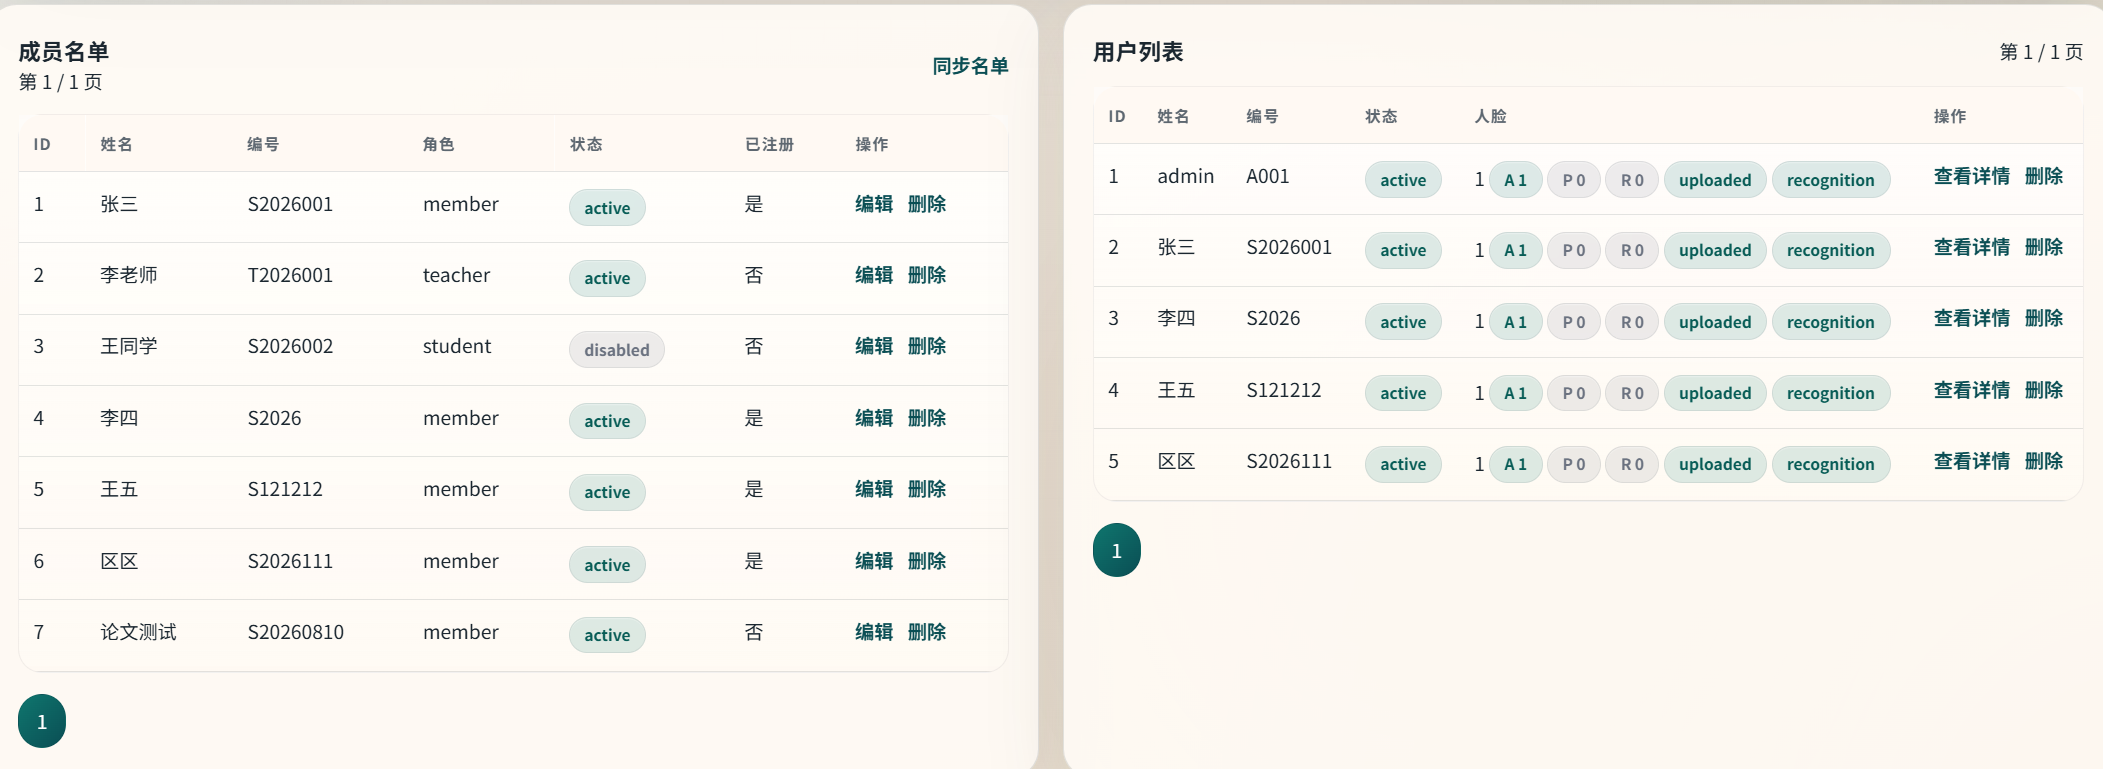
\includegraphics[width=0.86\textwidth]{figures/raspberry/image13.png}
\caption{图5.1 人员名单展示图}
\end{figure}

在当前测试数据中，左侧成员名单有7人，右侧用户列表有5人。右侧5人表示已经完成注册并激活账号。下文从创建人员名单开始说明用户模块的主要流程。

首先，用户想要使用本系统，管理员需要先在系统中添加对应成员。管理员添加成员名单的操作截图如下。

\begingroup
\small
\begin{longtable}{|>{\raggedright\arraybackslash}p{0.460\textwidth}|>{\raggedright\arraybackslash}p{0.460\textwidth}|}
\hline
(a)添加人员名单 & (b)显示添加成功 \\
\hline
\end{longtable}
\endgroup

\par\centerline{图5.2 管理员添加成员名单截图}
图5.2中，笔者添加了“论文测试2”这一测试成员。添加完成后，页面返回成功提示。该成员后续若想进入用户门户，便得使用姓名、编号和初始密码完成账号激活。

接着，用户门户由/portal/*页面路由和/api/portal/*业务接口组成。在用户首次注册时，需要填写姓名、学号或工号、初始密码、新密码和确认密码。提交后，后端处理时会先同步成员名单，再依次校验输入的所有元素。全部通过后，系统在users表中创建账号，并把用户ID写入浏览器Session，随后引导用户进入人脸采集流程。

首次注册页面运行效果如图5.3所示。

\begin{figure}[H]
\centering
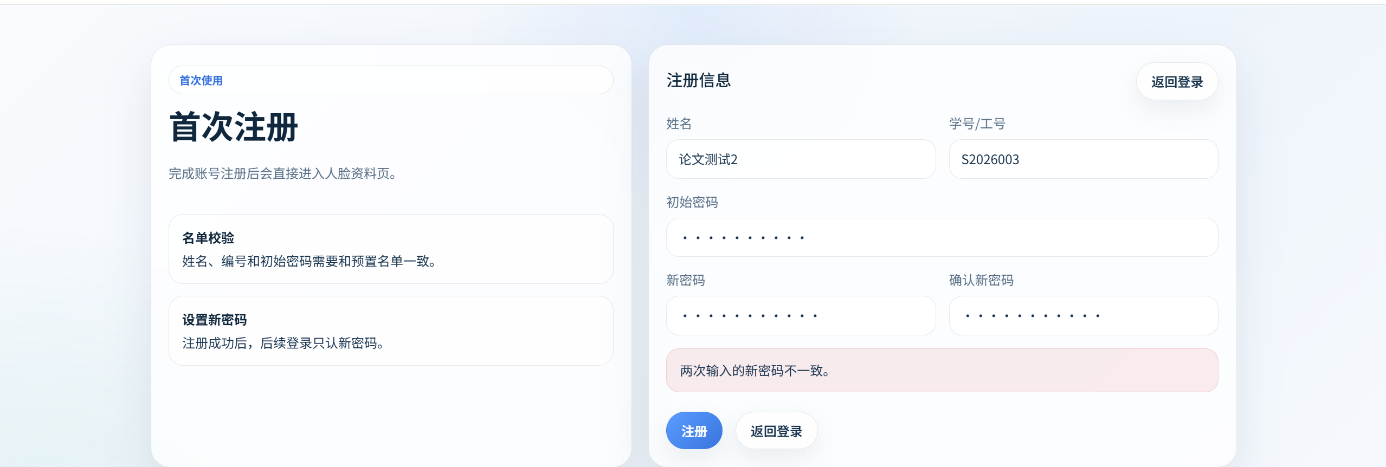
\includegraphics[width=0.86\textwidth]{figures/raspberry/image16.png}
\caption{图5.3 账号注册激活页面}
\end{figure}

用户完成首次注册后，后续登录只使用正式密码。登录成功后，系统进入用户中心，展示姓名、编号、角色、最近人脸档案状态、是否可用于识别、最近上传时间、审核原因和重新上传限制。用户中心主要让普通用户知道自己的资料处于什么状态：尚未上传、待审核、审核通过或审核未通过。如果最近照片被驳回，页面会展示驳回原因和备注；如果已有审核通过档案，同时又提交了新照片等待审核，终端仍继续使用之前通过的档案。用户中心运行效果如图5.4所示。

\begin{figure}[H]
\centering
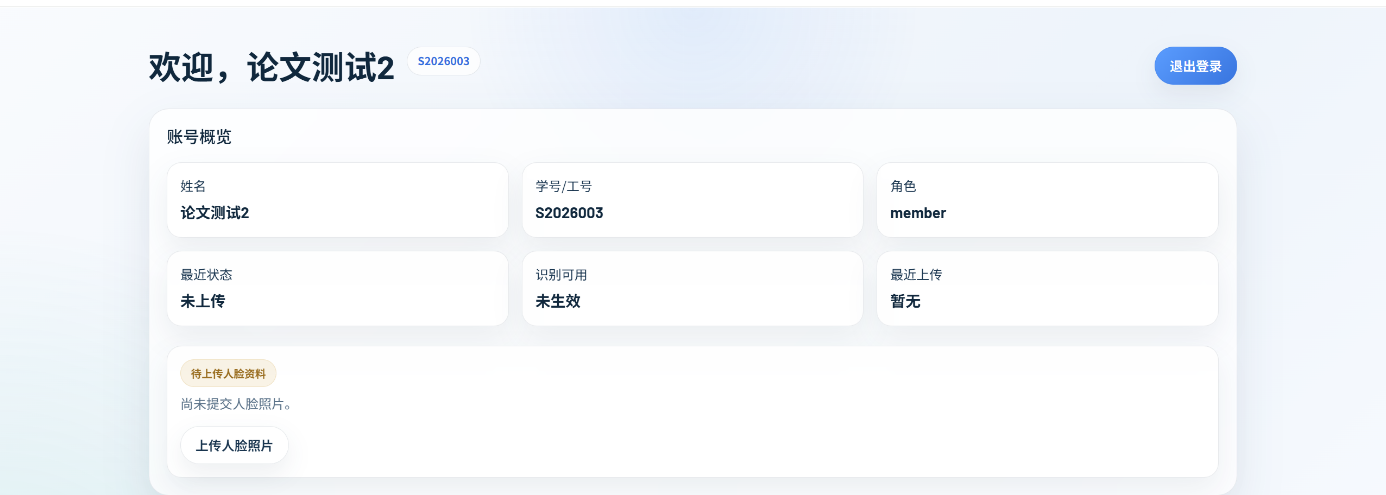
\includegraphics[width=0.86\textwidth]{figures/raspberry/image17.png}
\caption{图5.4 用户个人中心}
\end{figure}

接着，用户需要上传自己的人脸资料。人脸采集部分采用动作挑战和质量校验结合的方式。用户进入人脸采集页后，前端通过/api/liveness/challenges创建动作挑战会话，后端生成挑战ID、过期时间和动作序列。用户每次点击抓拍时，前端把当前摄像头画面以图片数据提交给后端；后端解码图片、检测人脸、计算姿态、校验同人一致性，并返回当前步骤是否通过。当前步骤通过后，挑战状态推进到下一步；失败时，系统返回具体原因，例如未检测到人脸、多人入镜、需要正脸、需要轻微侧转或中途换人。上传人脸页面运行效果如图5.5所示。

\begin{figure}[H]
\centering
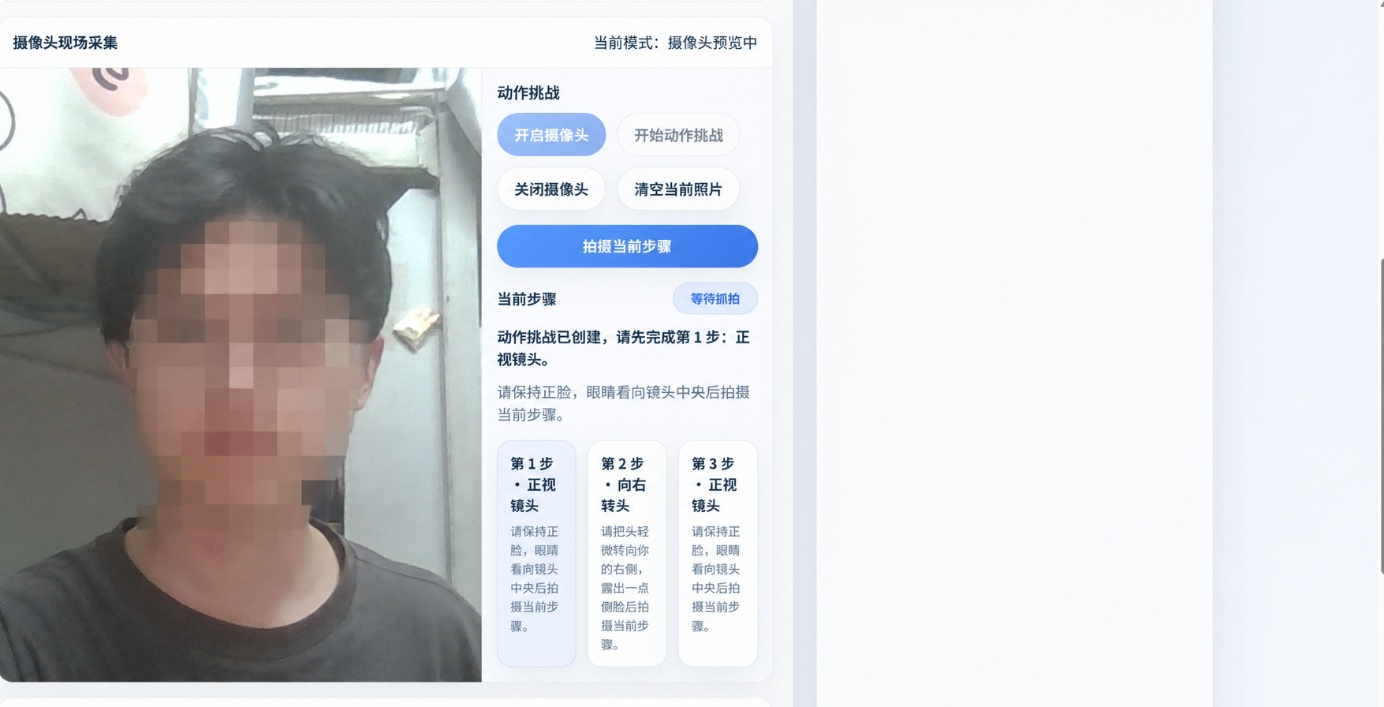
\includegraphics[width=0.86\textwidth]{figures/raspberry/image18.jpeg}
\caption{图5.5上传人脸资料界面}
\end{figure}

质量校验流水线的实现重点是先构建上下文，再按规则逐项拦截。系统先从图片字节解码得到图像矩阵，再完成人脸检测和关键点提取，并把这些中间结果保存在上下文对象中。后续校验器复用同一个上下文，避免每个规则重复检测人脸。清晰度检测使用Laplacian方差：

\begin{equation*}
Q_{\mathrm{blur}}=\operatorname{Var}(\nabla^2 G)\tag{5.1}
\end{equation*}

其中，G为人脸区域灰度图像。亮度检测使用人脸区域灰度均值，姿态检测使用眼睛、鼻尖和嘴部关键点的几何关系，翻拍风险检测结合矩形边框、周期纹理和高亮反光比例。质量校验流程如图5.6所示。

\begin{figure}[H]
\centering
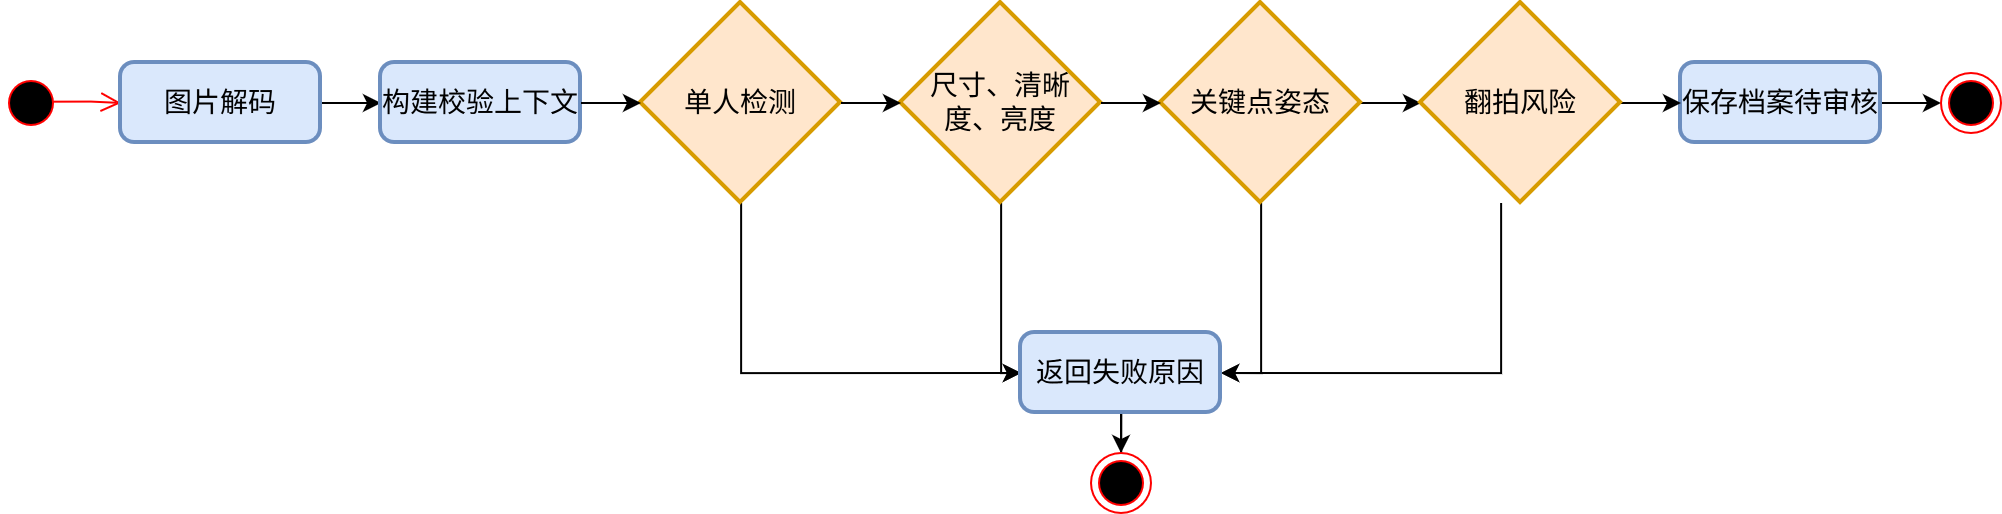
\includegraphics[width=0.86\textwidth]{figures/raspberry/image19.png}
\caption{图5.6 质量校验流程图}
\end{figure}

在图5.6的拦截顺序中，单人检测放在最前面，因为后续人脸尺寸、关键点和特征提取都依赖单张人脸；尺寸、清晰度和亮度用于控制基础图像质量；关键点和姿态用于保证注册照适合后续对齐和特征提取；翻拍风险用于减少纸张或屏幕照片进入审核环节的可能。校验通过后，系统保存图片文件并写入face\_profiles表，新档案默认状态为pending，等待管理员审核。图5.7为全部质量校验通过后的反馈。

\begin{figure}[H]
\centering
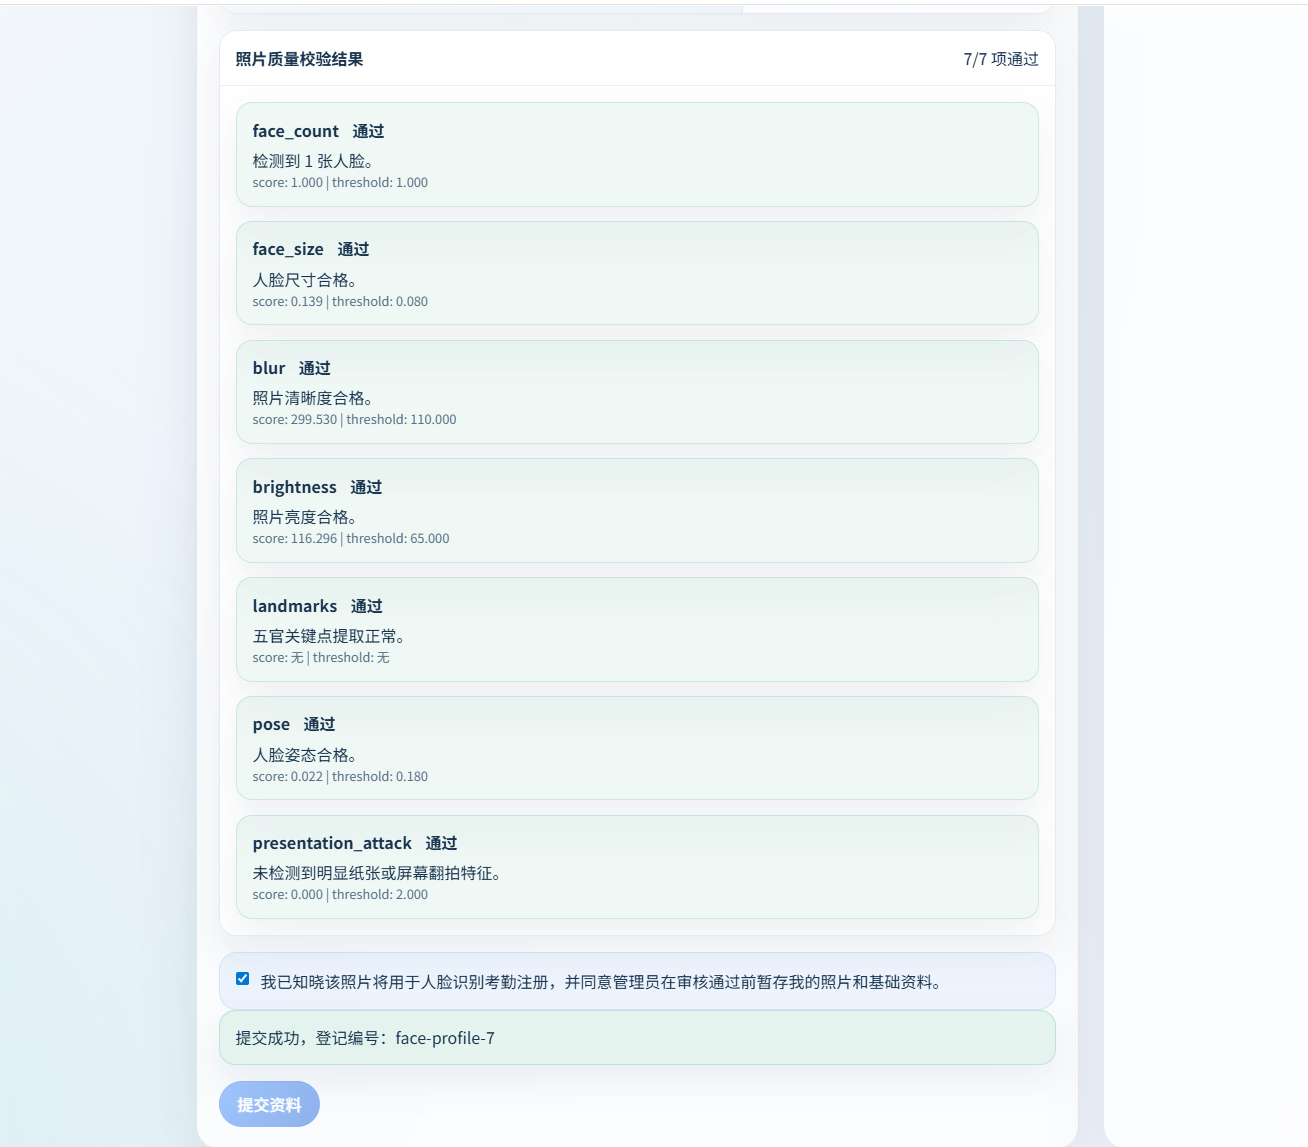
\includegraphics[width=0.86\textwidth]{figures/raspberry/image21.png}
\caption{图5.7 质量校验通过反馈图}
\end{figure}

提交人脸资料之后，用户返回个人中心，可以看到自己提交的人脸审核情况。图5.8中，人脸照片已经上传到系统，但还没有经过管理员审核通过，页面同时还提示需多长时间才能再次提交。

\begin{figure}[H]
\centering
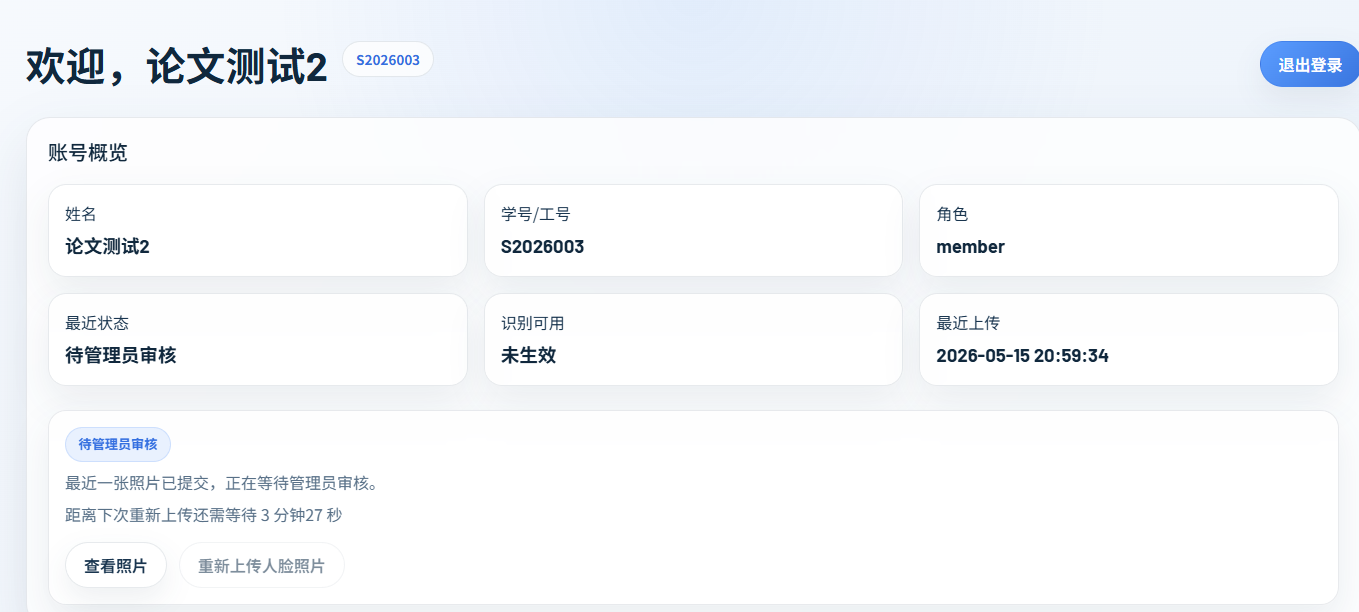
\includegraphics[width=0.86\textwidth]{figures/raspberry/image22.png}
\caption{图5.8 个人中心上传人脸后的反馈}
\end{figure}

\section{树莓派侧人脸识别与考勤写入实现}
\begin{figure}[H]
\centering
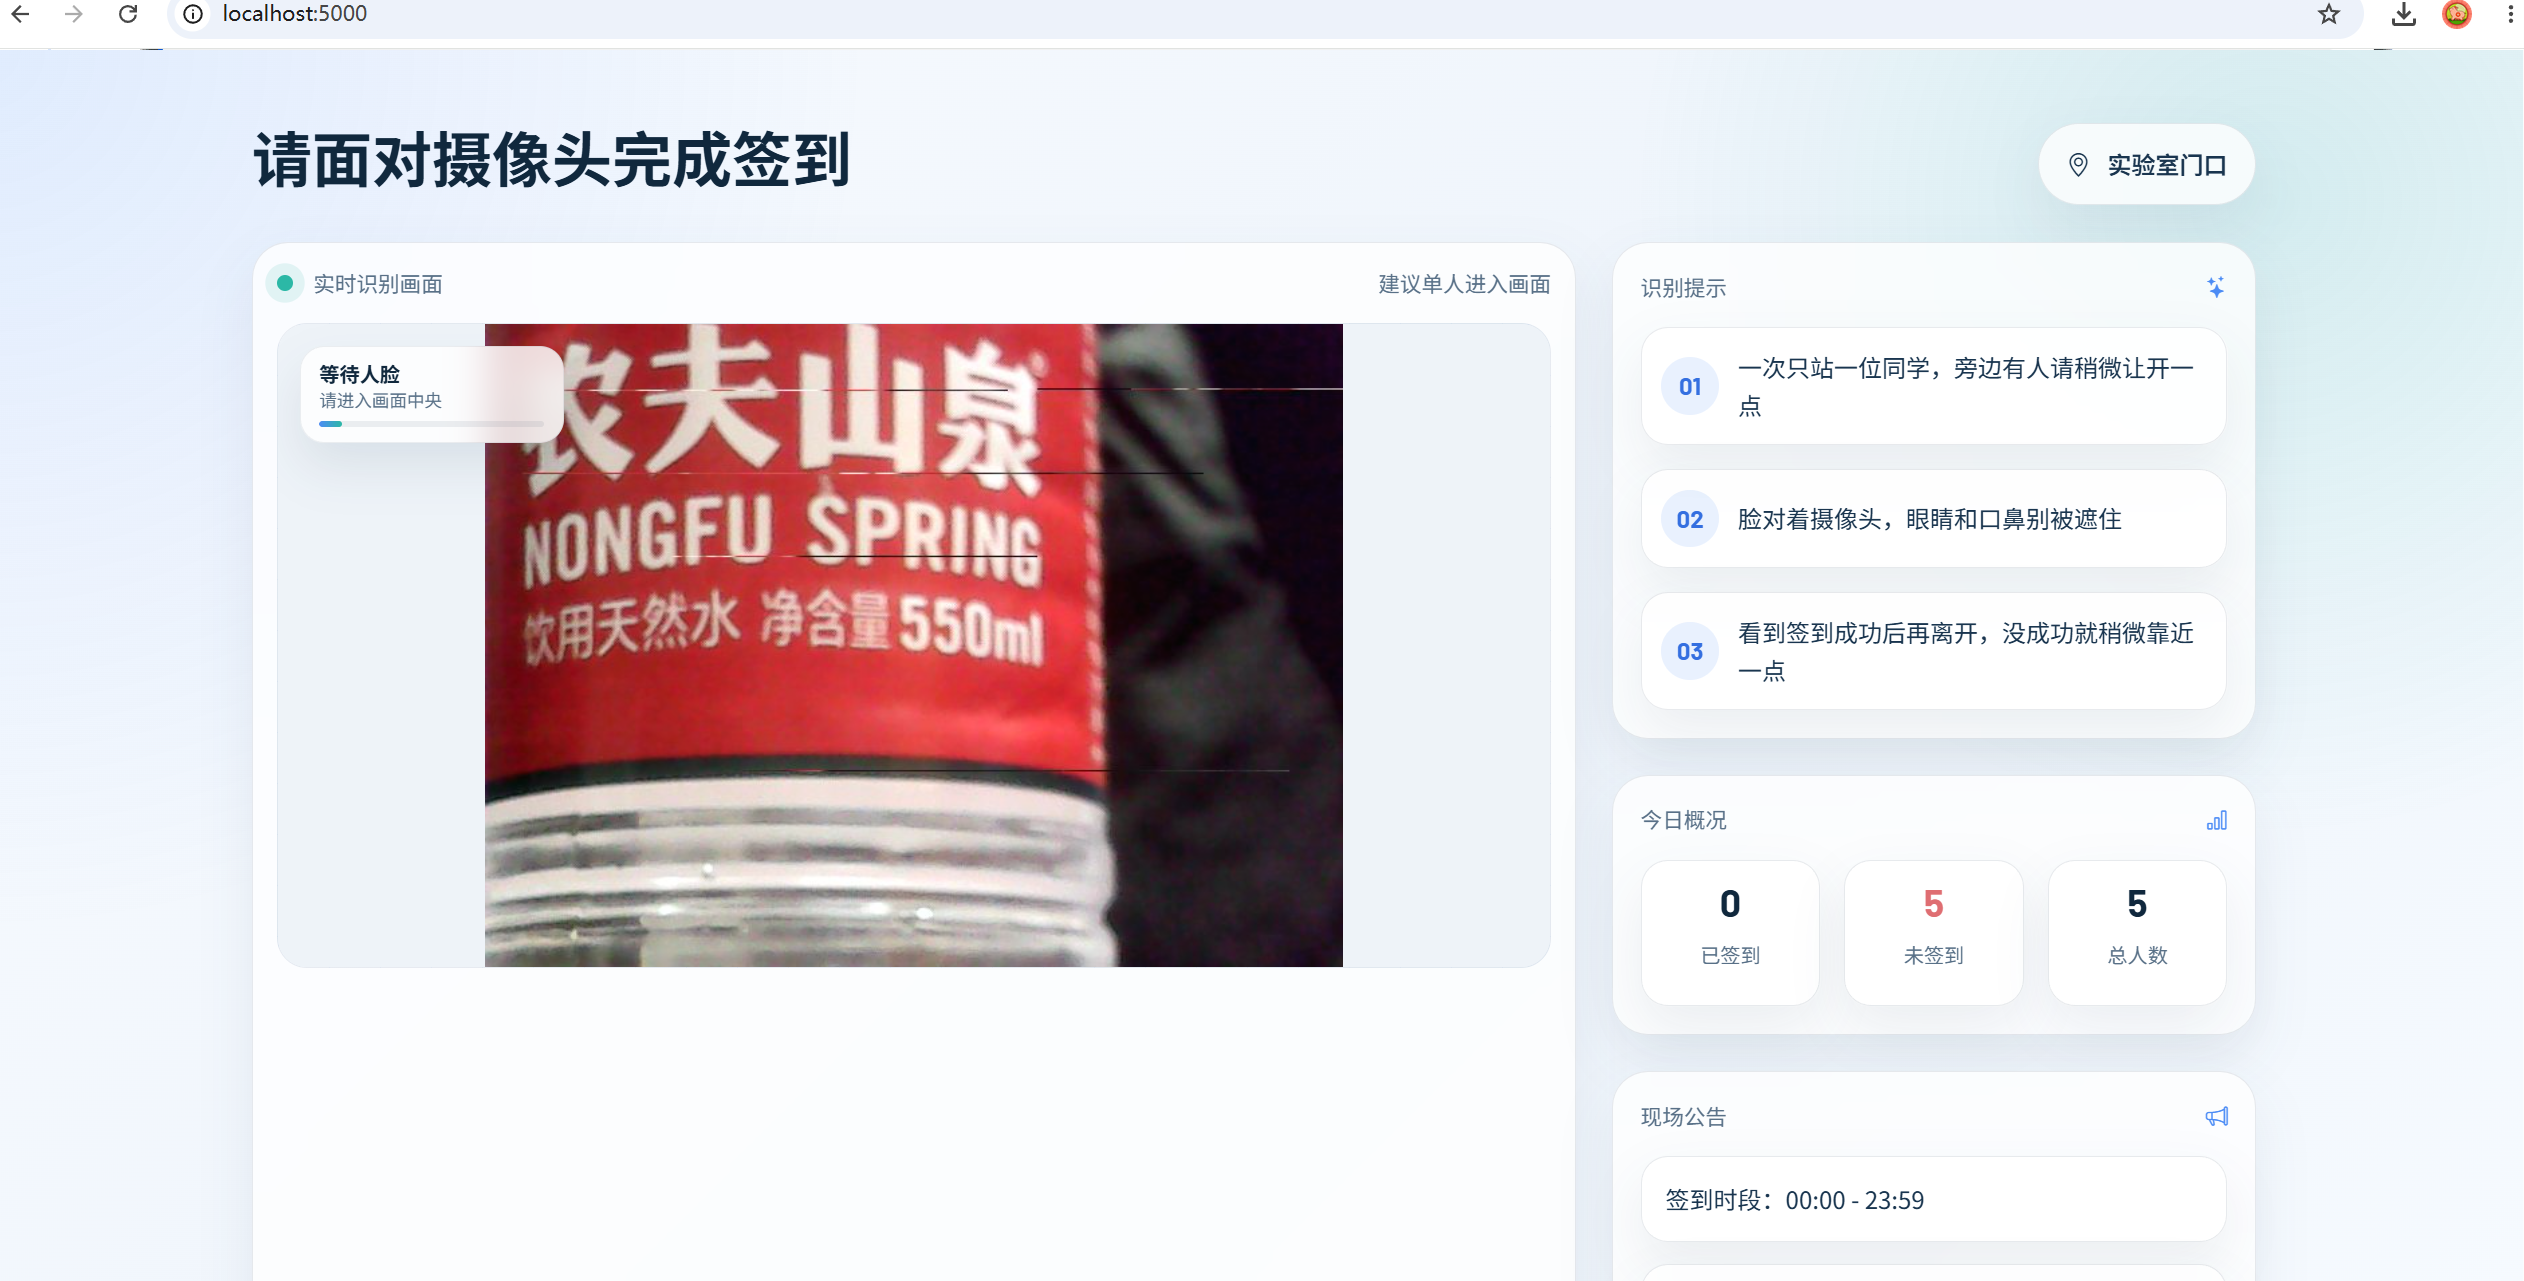
\includegraphics[width=0.86\textwidth]{figures/raspberry/image23.png}
\caption{图5.9 终端实时识别页面}
\end{figure}

终端识别页面由templates/user\_screen.html渲染，本地浏览器访问根路径/即可进入。页面左侧展示MJPEG摄像头流，右侧展示当日考勤状况。终端页面的数据由接口低频刷新：/api/terminal/status返回识别进度，/api/terminal/screen-data返回今日签到统计、设备位置和公告信息。终端实时识别页面运行效果如图5.9所示。

终端摄像头服务分为采集线程和识别线程。采集线程负责打开摄像头、设置分辨率与帧率、读取原始帧，并按配置完成缩放、镜像、旋转和JPEG编码，随后供MJPEG视频流使用。识别线程则按系统配置频率取共享缓冲区中的最新帧，完成YuNet检测、活体判断、SFace特征提取、身份匹配和考勤规则判断这一系列操作。两个线程之间只传递最新帧，鉴于树莓派的处理性能，只能让旧帧被覆盖后直接丢弃，这样可以避免识别耗时波动造成画面积压，且基本不会影响整体判断。

终端运行时的线程交互如图5.10所示。该图展示了页面视频流、采集线程、识别线程、识别引擎和数据库之间的关系。

\begin{figure}[H]
\centering
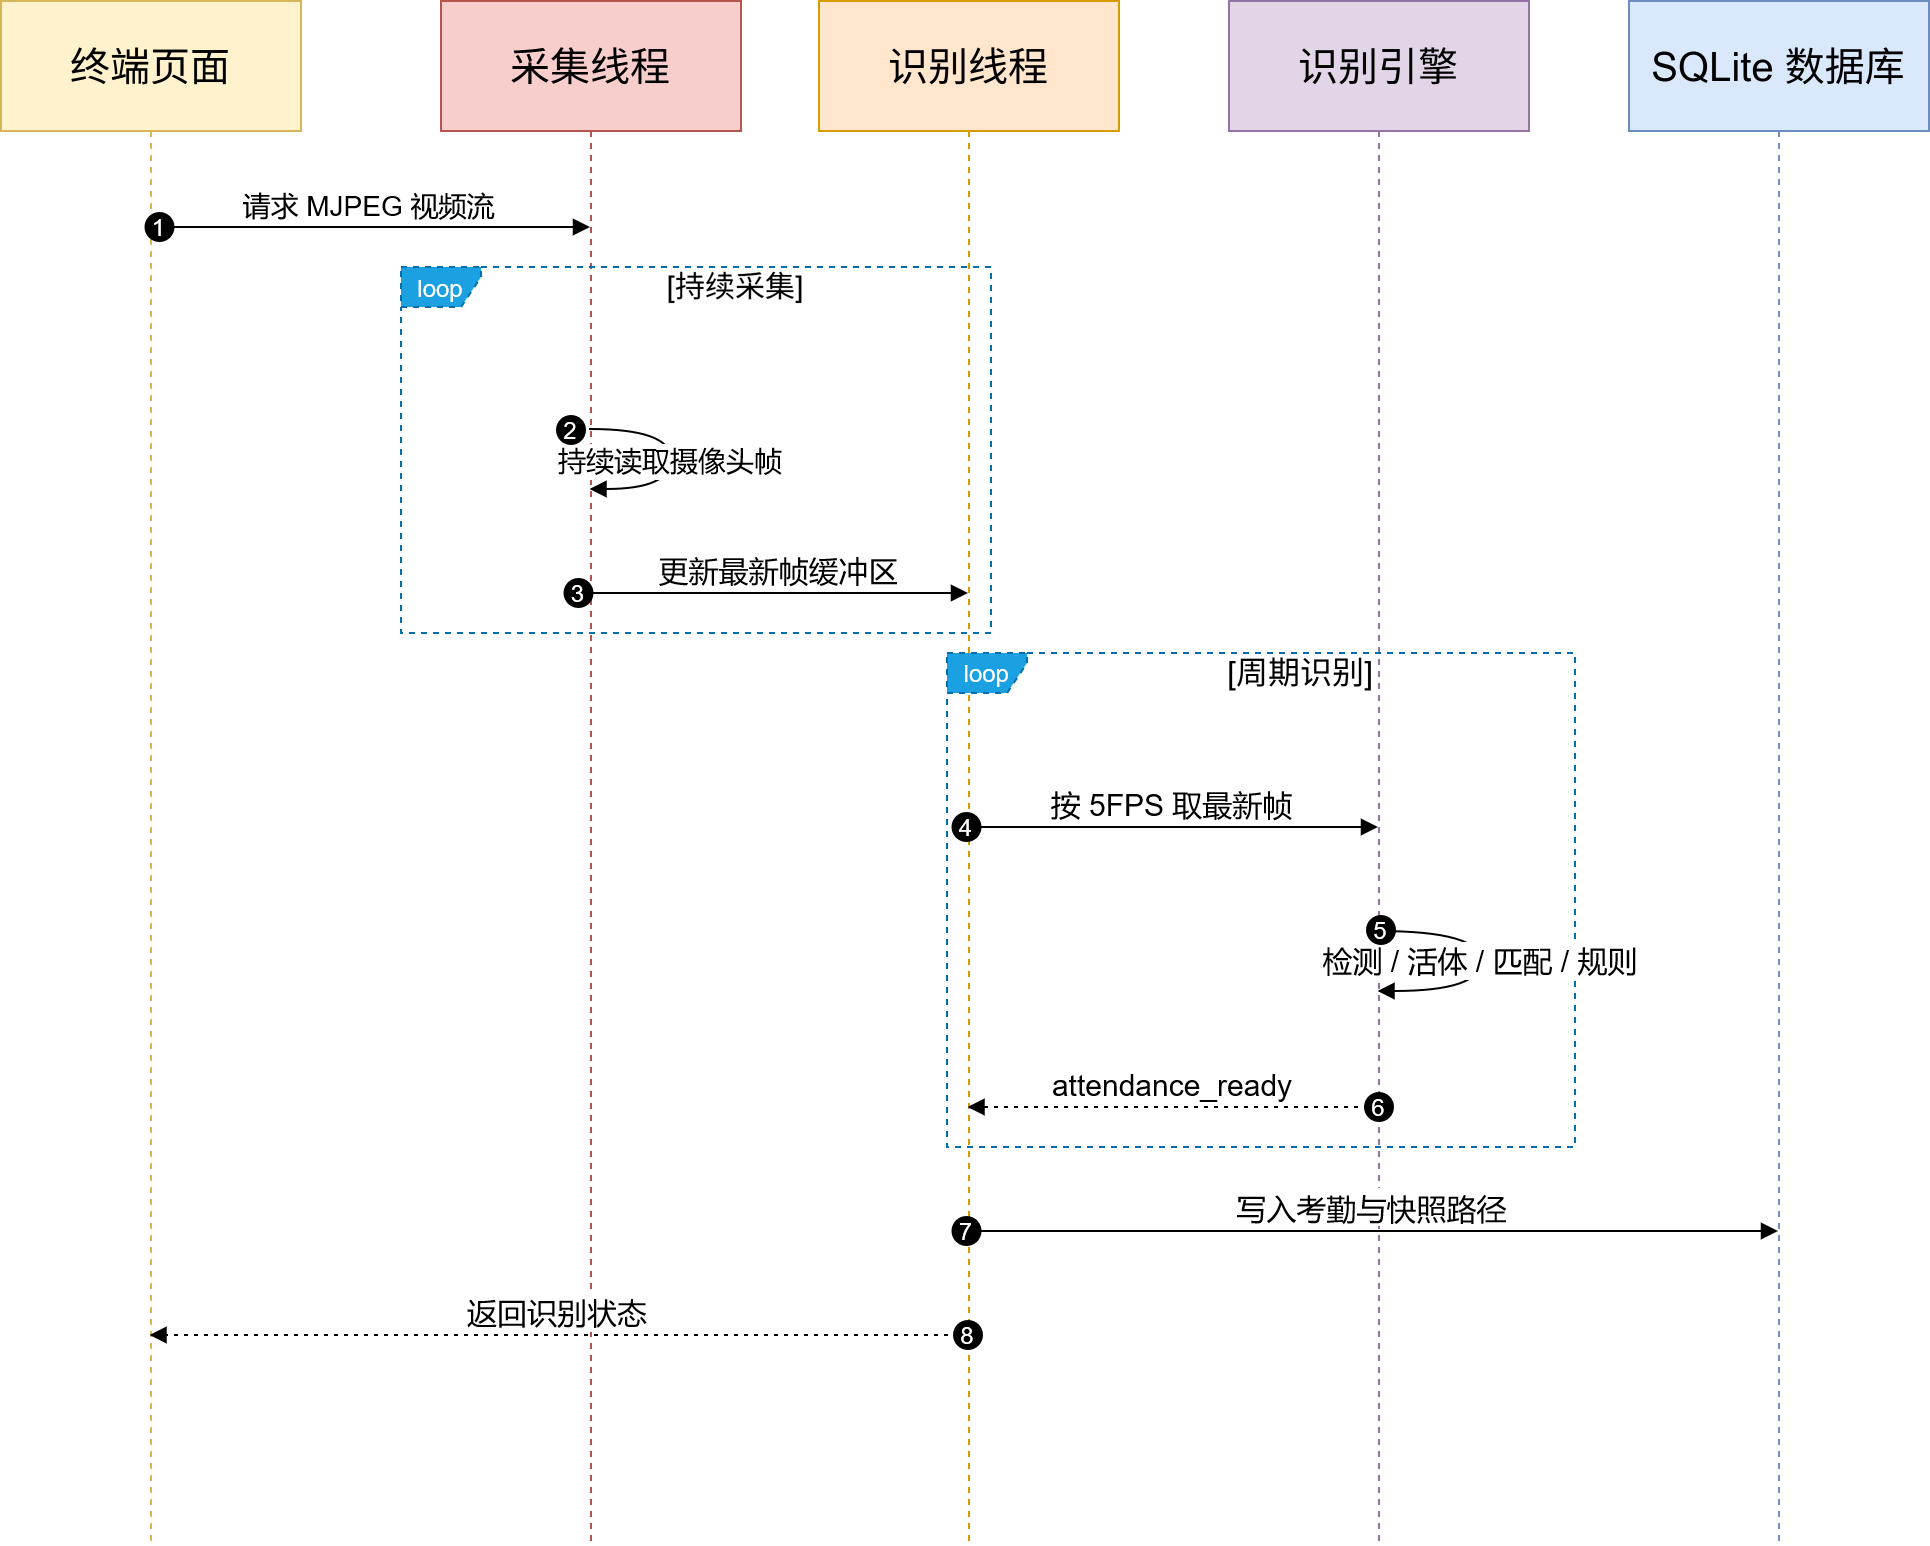
\includegraphics[width=0.86\textwidth]{figures/raspberry/image24.png}
\caption{图5.10 终端识别与签到时序图}
\end{figure}

图5.10中的关键点是视频流和识别推理不互相等待。终端页面请求视频流后，采集线程持续产生MJPEG帧；识别线程以配置的5FPS频率取最新帧进行处理，其中识别引擎先从SQLite加载曾经审核通过的人脸档案信息，然后内存中缓存该用户各种信息以及人脸特征向量。单帧识别时，系统依次执行前文提到的人脸匹配、活体检测。这两项通过后，就要进入本考勤系统设置的规则校验（是否重复签到、是否在考勤时间段）。全部条件通过后，识别结果被标记为attendance\_ready，即签到成功。

识别线程给出可签到结果后，，Repository向attendance\_records表写入签到记录，并把当前帧保存为现场快照。快照按日期分目录保存，文件名中包含时间和用户编号。终端页面随后显示短暂的成功提示，状态接口也会返回“已签到”等进度信息，方便页面侧刷新。

\begin{figure}[H]
\centering
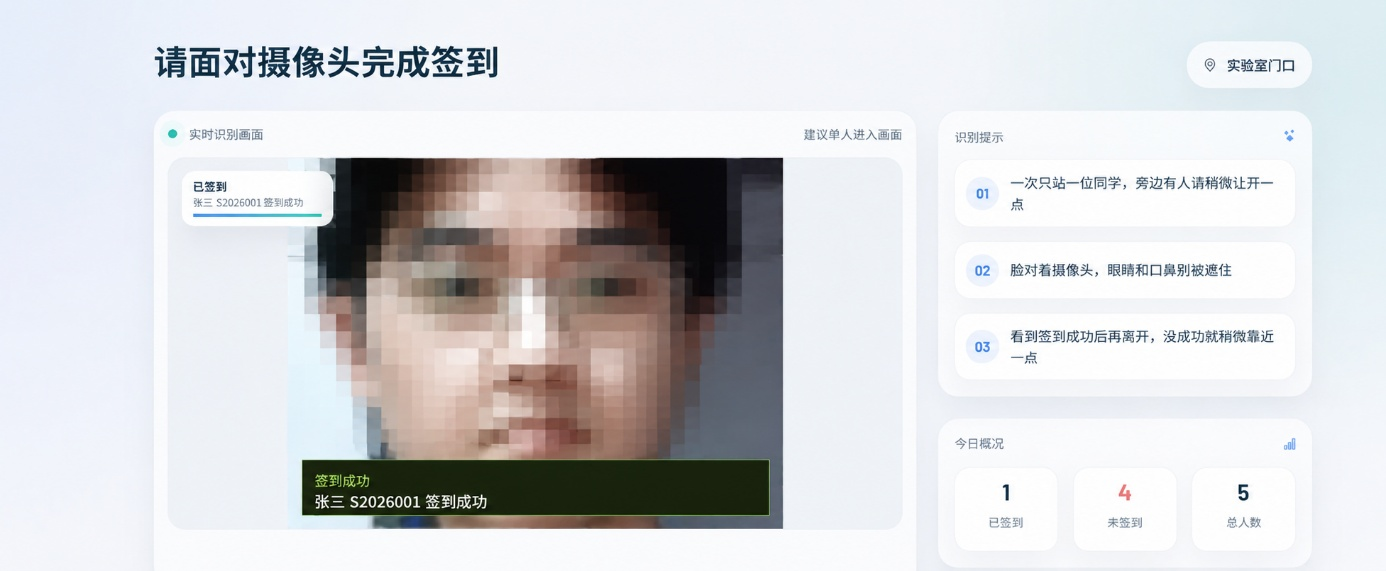
\includegraphics[width=0.86\textwidth]{figures/raspberry/image26.jpeg}
\caption{图5.11 签到成功效果图}
\end{figure}

为了让终端能够连续运行，摄像头服务对几个异常状态做了处理。摄像头打开失败时，页面显示中文占位画面并提示检查摄像头编号或权限；连续读帧失败时，服务释放摄像头句柄并在下一轮尝试重新连接；管理员审核通过的新档案通过识别库定时重载进入内存，不要求重启服务；签到快照按保留天数清理，避免树莓派磁盘空间长期被图片占用。这些设定也能够体现本系统的工作量，也增强了本系统的健壮性。

\section{管理员接口与远程管理实现}
管理员接口挂载在/api/admin路径下，供Windows管理端通过Tailscale访问。管理端请求必须携带管理员Token，可放在Authorization: Bearer \textless{}token\textgreater{}请求头中，也兼容X-Admin-Token。接口返回结构统一使用ok、data、items和total等字段，便于Windows端页面处理。设备状态类接口返回基础信息、健康状态、性能指标和配置重载结果。具体情况如下图所示。

\begin{figure}[H]
\centering
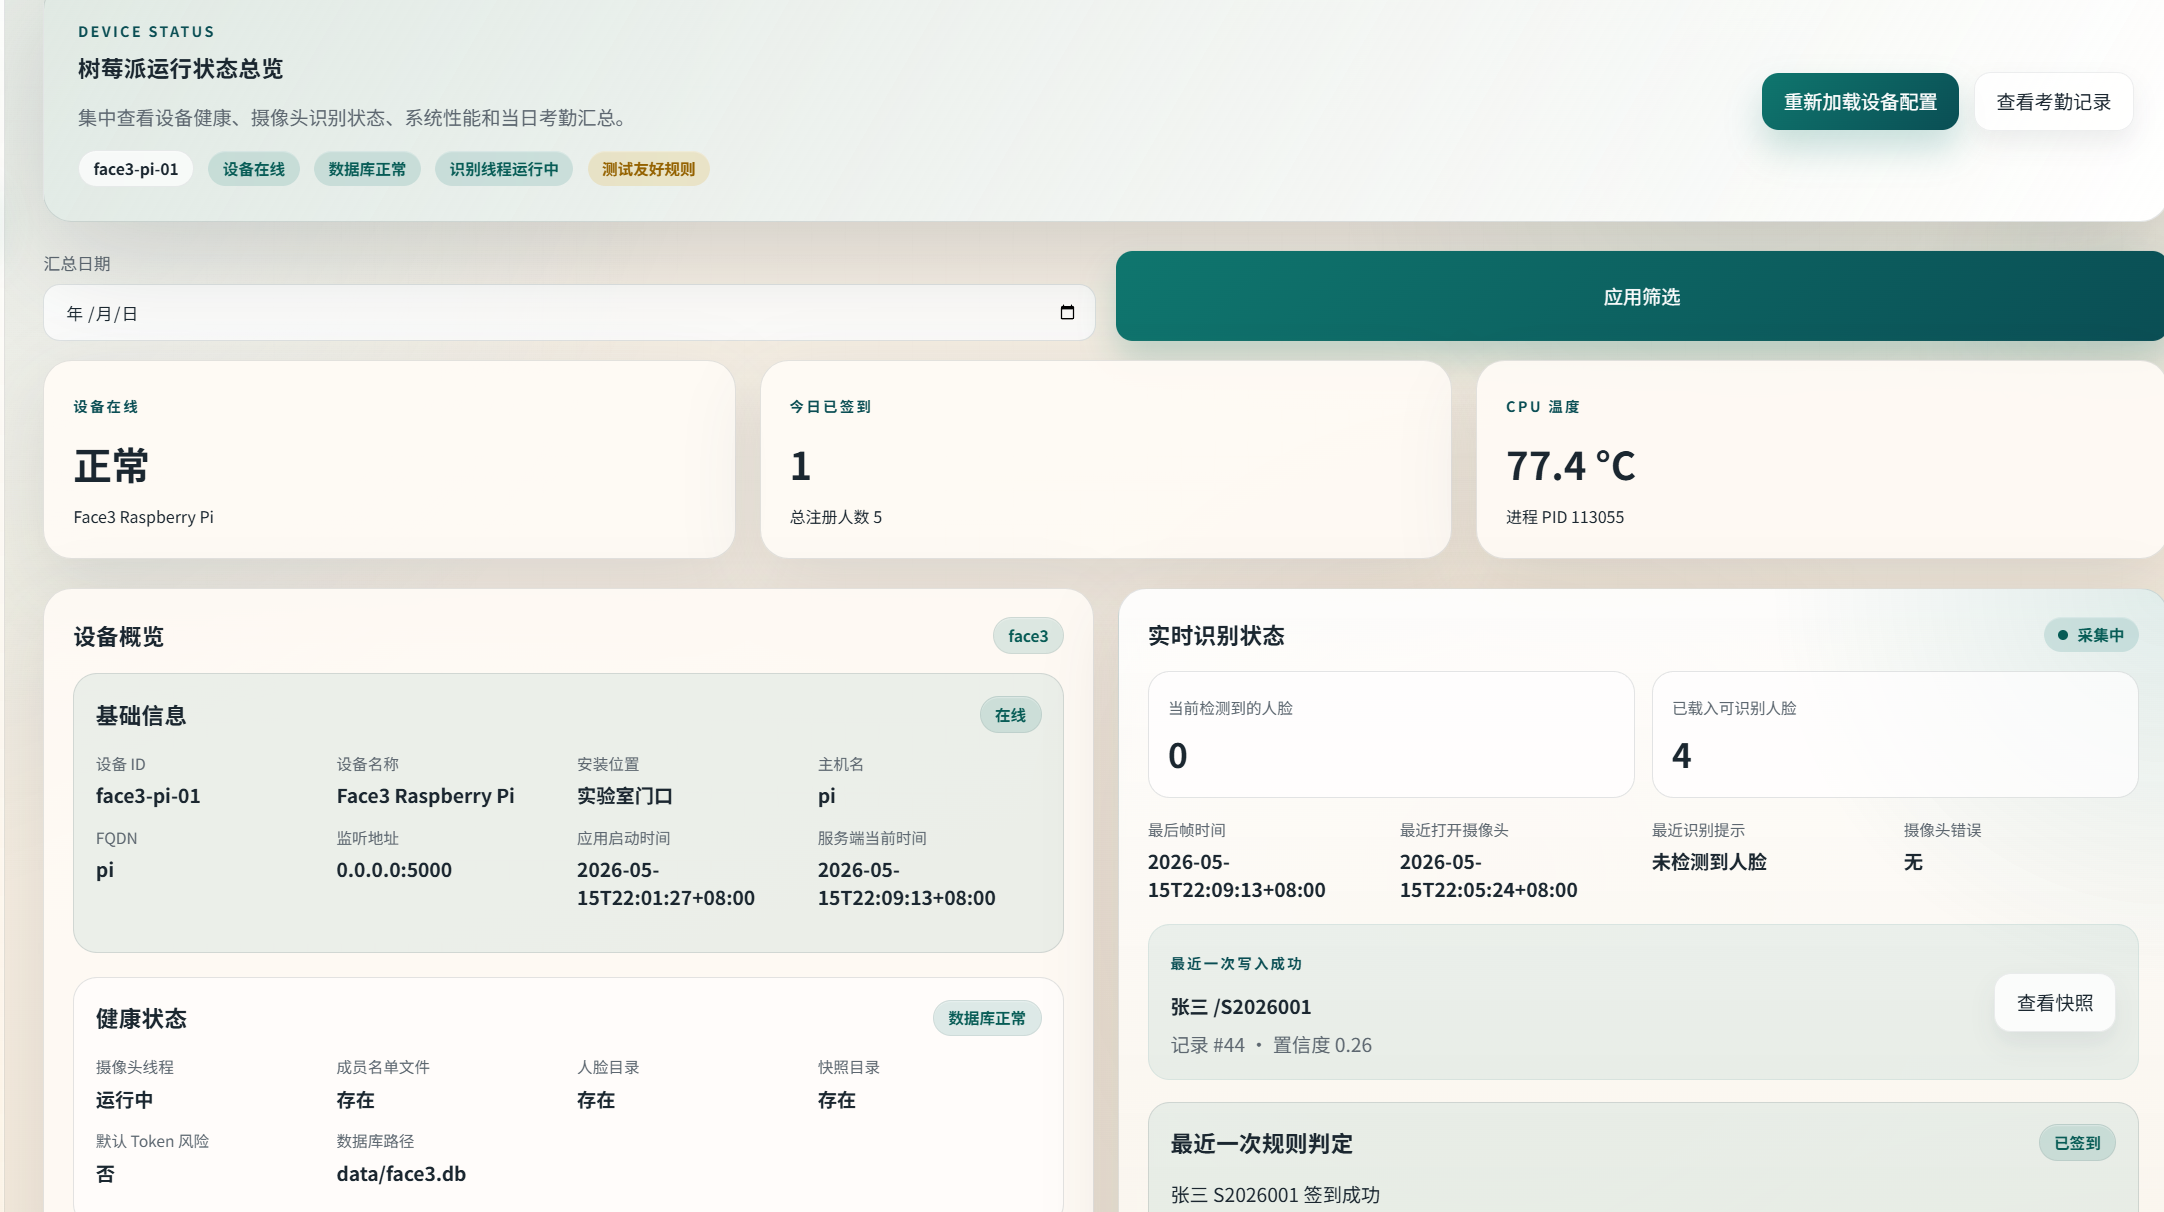
\includegraphics[width=0.86\textwidth]{figures/raspberry/image27.png}
\caption{图5.12 树莓派设备信息上半区域}
\end{figure}

\begin{figure}[H]
\centering
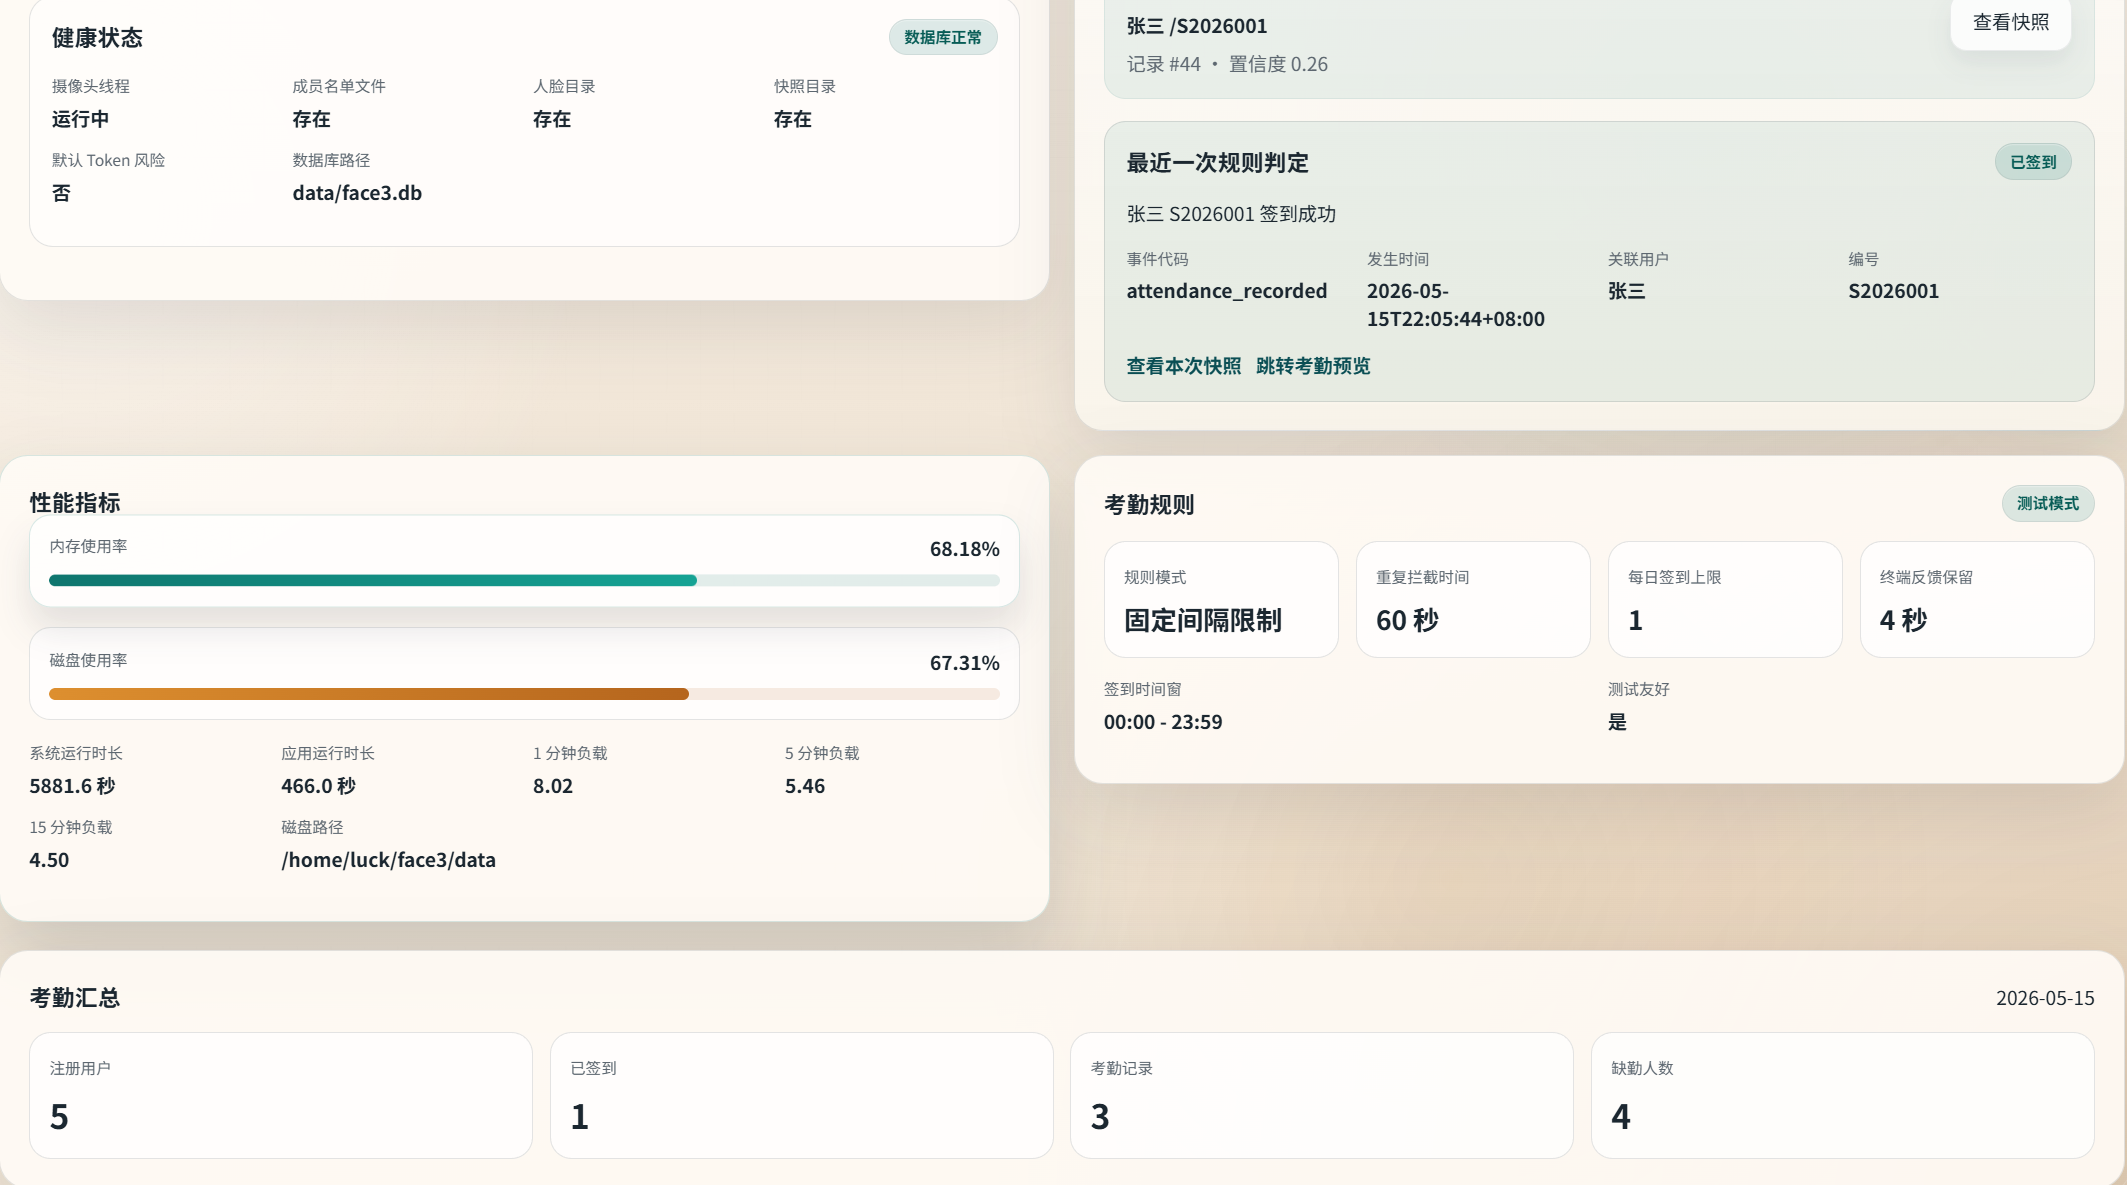
\includegraphics[width=0.86\textwidth]{figures/raspberry/image28.png}
\caption{图5.13 树莓派设备信息下半区域}
\end{figure}

成员与用户接口体现了本系统中一开始设定的“初始名单”和“注册账号”的区别。初始成员名单表示管理员允许哪些人注册，用户账号表示哪些成员已经完成首次注册。成员接口支持同步CSV名单、查询成员、新增成员和更新成员状态；用户接口支持查询用户列表、查看用户详情、更新用户状态和重置密码。两类接口分开后，本系统可以表达多个中间状态：名单中存在但尚未注册、已注册但未上传人脸、已上传但待审核、审核通过可识别、审核驳回需重新提交。管理员端就可以根据这些状态筛选用户并进行处理。由于图5.1已经展示过人员名单，此处不再重复放图。

人脸档案审核是管理员端的核心业务之一。系统支持按用户、编号和审核状态查询人脸档案，也支持查看图片、审核通过、审核驳回、重新置为待审核和删除。审核通过后，review\_status变为approved，终端识别库下次重载时即可加载；审核驳回后，系统保存驳回原因、备注、审核人和审核时间，并写入驳回历史。管理员人脸审核运行效果如图5.14所示。

\begin{figure}[H]
\centering
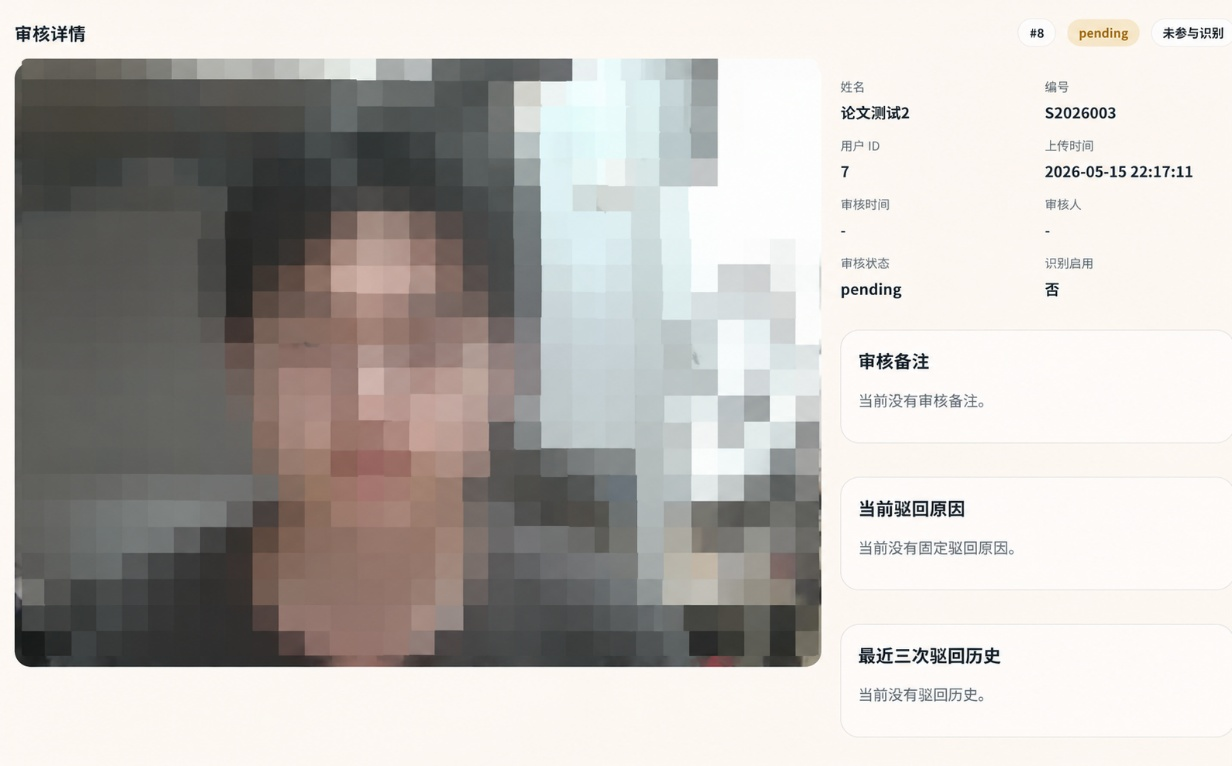
\includegraphics[width=0.86\textwidth]{figures/raspberry/image29.jpeg}
\caption{图5.14 管理员审核人脸界面上部分}
\end{figure}

图5.14可以看到在图5.5上传的人脸资料，以及对应人员账号的详细信息。页面继续向下滚动后，管理员可以对该人脸资料进行审核。图5.15演示的是驳回操作，审核人可以选择驳回理由。

\begin{figure}[H]
\centering
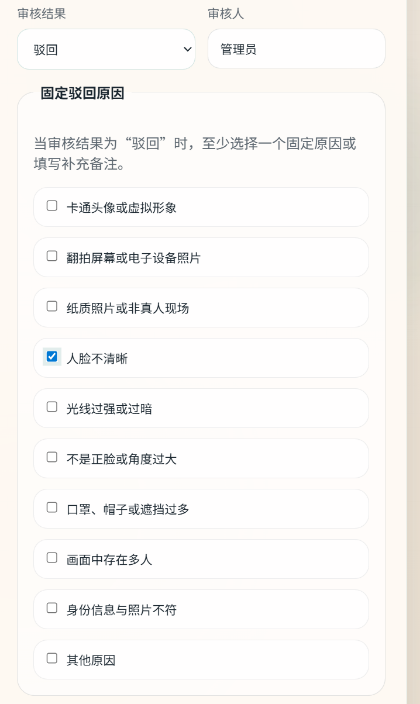
\includegraphics[width=0.86\textwidth]{figures/raspberry/image30.png}
\caption{图5.15 管理员审核人脸界面中部分}
\end{figure}

选择驳回理由后，管理员点击提交审核结果，如图5.16所示。

\begin{figure}[H]
\centering
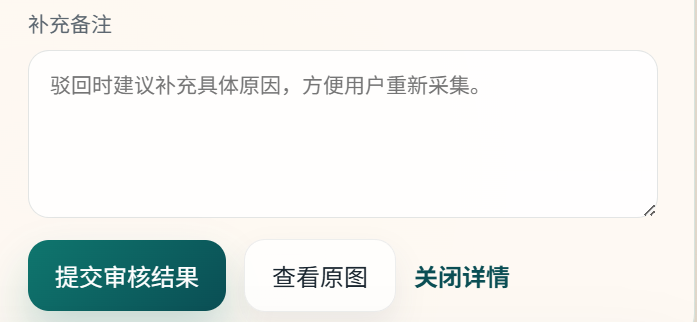
\includegraphics[width=0.86\textwidth]{figures/raspberry/image31.png}
\caption{图5.16 管理员审核人脸界面下部分}
\end{figure}

审核完成后，用户重新登录账号，可以在用户中心看到自己上传的人脸资料被审核的情况，如图5.17所示。

\begin{figure}[H]
\centering
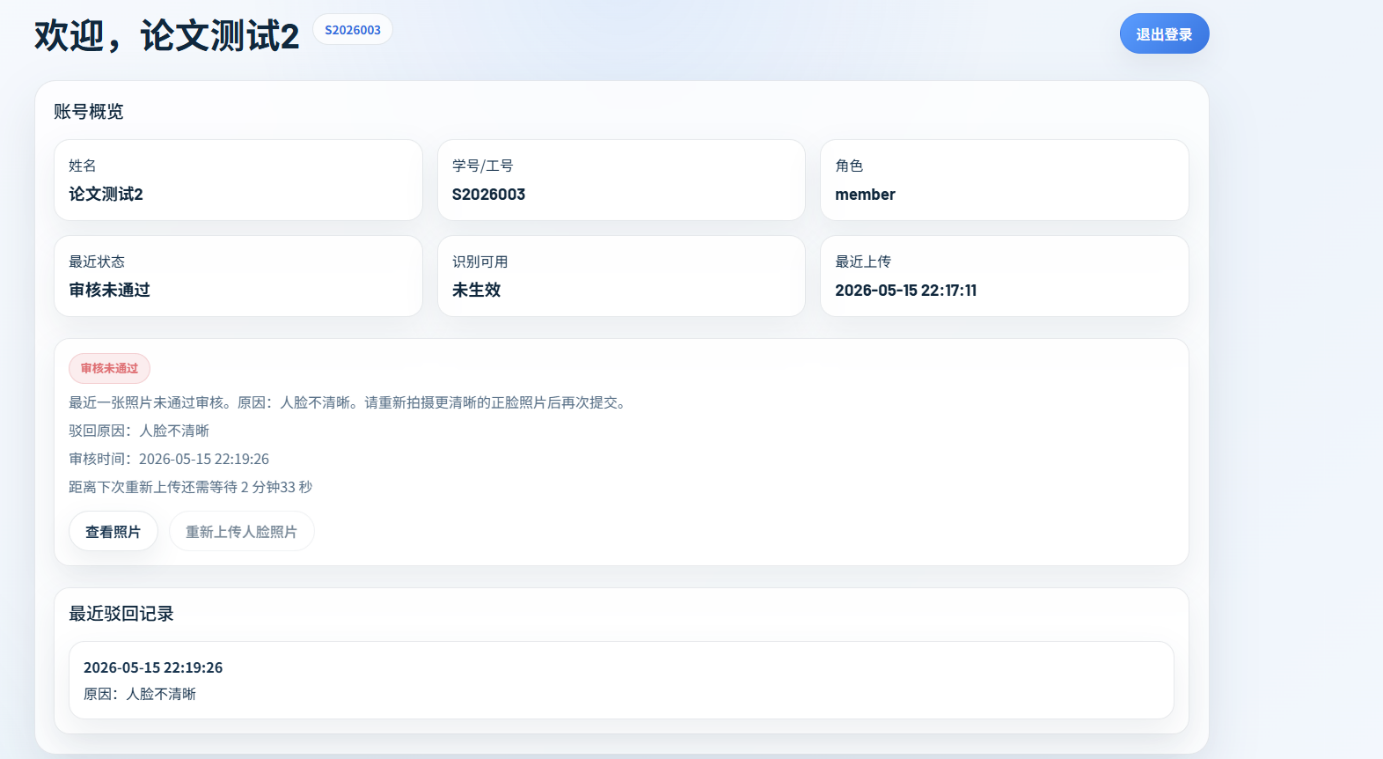
\includegraphics[width=0.86\textwidth]{figures/raspberry/image32.png}
\caption{图5.17 用户中心查看被审核情况}
\end{figure}

考勤接口支持按日期、编号和姓名查询记录，同时支持今日汇总和签到快照访问。查询结果包含用户ID、姓名、编号、签到类型、签到时间、快照路径、快照是否可用和识别置信度。Windows管理端可以根据这些字段展示考勤表格，也可以通过本地代理方式展示现场快照。管理员考勤记录查询运行效果如图5.18所示。

\begin{figure}[H]
\centering
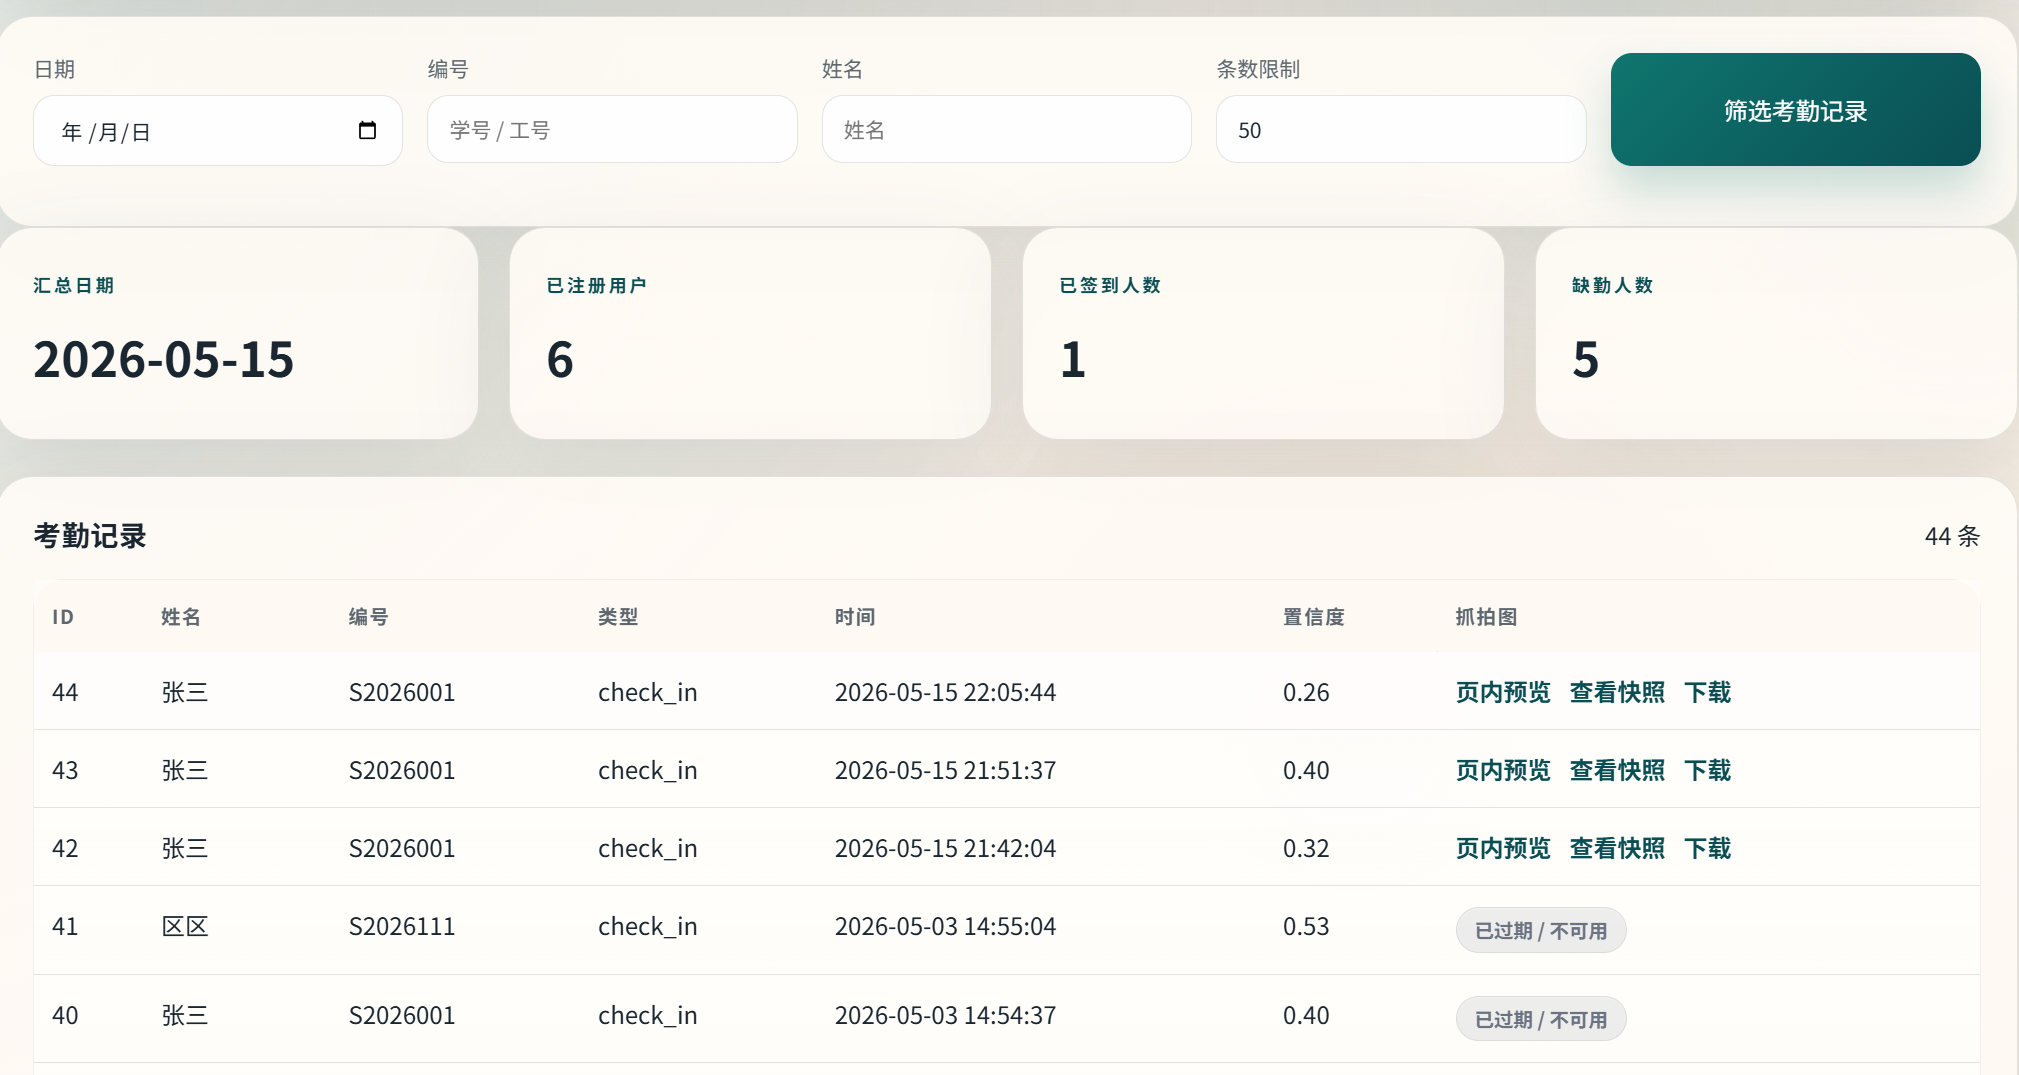
\includegraphics[width=0.86\textwidth]{figures/raspberry/image33.png}
\caption{图5.18 管理员查看考勤记录}
\end{figure}

\section{测试过程与结果分析}
系统测试围绕已实现功能进行，主要检查三个方面：普通用户能否从名单准入开始完成首次注册、动作挑战、人脸提交和审核状态查看；管理员能否通过远程接口完成成员、用户、人脸档案和考勤记录管理；终端能否在树莓派端完成实时视频展示、人脸识别、活体判断、考勤写入和快照保存。测试环境配置如表5.6所示。

\begingroup
\small
\begin{longtable}{|>{\raggedright\arraybackslash}p{0.460\textwidth}|>{\raggedright\arraybackslash}p{0.460\textwidth}|}
\caption{表5.6 测试环境配置}\\
\hline
项目 & 配置 \\
\hline
终端设备 & Raspberry Pi 3B+，1GB内存 \\
\hline
操作系统 & Raspberry Pi OS 64位 \\
\hline
Python版本 & Python 3.9 \\
\hline
摄像头 & 普通USB摄像头 \\
\hline
摄像头配置 & 1280×720，15FPS \\
\hline
识别模型 & OpenCV YuNet + SFace \\
\hline
活体模型 & OpenVINO anti-spoof-mn3，CPU推理 \\
\hline
数据库 & SQLite，本地文件data/face3.db \\
\hline
Web服务 & FastAPI + Uvicorn，监听5000端口 \\
\hline
\end{longtable}
\endgroup

功能测试采用黑盒测试方法，按照用户实际使用路径设计用例。账号与注册采集测试如表5.7所示。

\begingroup
\small
\begin{longtable}{|>{\raggedright\arraybackslash}p{0.230\textwidth}|>{\raggedright\arraybackslash}p{0.230\textwidth}|>{\raggedright\arraybackslash}p{0.230\textwidth}|>{\raggedright\arraybackslash}p{0.230\textwidth}|}
\caption{表5.7 账号与注册采集测试}\\
\hline
模块 & 测试步骤 & 预期结果 & 结果 \\
\hline
首次注册 & 输入名单中存在的姓名、编号、初始密码和合规新密码 & 注册成功，进入人脸采集页 & 通过 \\
\hline
登录 & 使用注册后的正式密码登录 & 登录成功，进入用户中心 & 通过 \\
\hline
动作挑战 & 按提示完成正脸、侧转、正脸三步抓拍 & 挑战通过并冻结可信注册照 & 通过 \\
\hline
姿态校验 & 正脸步骤提交明显侧脸照片 & 返回需要正脸提示 & 通过 \\
\hline
同人校验 & 挑战中途更换测试人员 & 返回身份变化提示 & 通过 \\
\hline
质量校验 & 提交多人、模糊、过暗或疑似翻拍照片 & 返回对应失败原因 & 通过 \\
\hline
\end{longtable}
\endgroup

从表5.7可以看出，注册端能够拦截不符合要求的输入和图片。名单校验可以阻止非名单成员注册；动作挑战可以要求用户按步骤完成现场采集；同人校验可以发现挑战中途换人的情况；质量校验会对多人、模糊、过暗和疑似翻拍等情况返回明确失败原因。对用户来说，失败原因可以直接指导重新拍摄；对系统来说，只有通过这些检查的照片才会进入待审核状态。

审核与终端签到测试如表5.8所示。

\begingroup
\small
\begin{longtable}{|>{\raggedright\arraybackslash}p{0.230\textwidth}|>{\raggedright\arraybackslash}p{0.230\textwidth}|>{\raggedright\arraybackslash}p{0.230\textwidth}|>{\raggedright\arraybackslash}p{0.230\textwidth}|}
\caption{表5.8 审核与终端签到测试}\\
\hline
模块 & 测试步骤 & 预期结果 & 结果 \\
\hline
管理员审核 & 将待审核人脸档案设置为approved & 记录状态变为approved，可被终端加载 & 通过 \\
\hline
审核驳回 & 管理员选择驳回原因并提交 & 写入驳回历史，用户中心可查看 & 通过 \\
\hline
已注册用户签到 & 审核通过用户正对摄像头 & 识别成功并写入考勤记录 & 通过 \\
\hline
未注册用户签到 & 未入库人员正对摄像头 & 返回未匹配，不写入记录 & 通过 \\
\hline
多人入镜 & 两人同时进入画面 & 返回多人入镜，不写入记录 & 通过 \\
\hline
重复签到 & 同一用户短时间内重复签到 & 返回冷却提示，不重复写入 & 通过 \\
\hline
\end{longtable}
\endgroup

从表5.8可以看出，审核状态能够正确影响终端识别库。待审核和驳回照片不会被终端加载，审核通过后才参与识别。终端识别能够区分已注册用户、未入库人员和多人入镜场景，重复签到冷却可以避免同一用户短时间内多次写入。结合运行截图来看，系统已经完成了从用户注册到管理员审核、从终端签到到管理员查询的主要流程。

性能测试主要关注树莓派端识别线程能否满足实际现场使用。终端识别线程目标频率为5FPS，对应每帧可用处理时间约200毫秒。根据系统运行观察和模型推理特点，单帧识别主要耗时分布如表5.9所示。

\begingroup
\small
\begin{longtable}{|>{\raggedright\arraybackslash}p{0.307\textwidth}|>{\raggedright\arraybackslash}p{0.307\textwidth}|>{\raggedright\arraybackslash}p{0.307\textwidth}|}
\caption{表5.9 识别线程主要阶段耗时}\\
\hline
处理阶段 & 耗时范围/ms & 说明 \\
\hline
YuNet人脸检测 & 30--50 & 输出人脸框、关键点和置信度 \\
\hline
OpenVINO活体推理 & 15--30 & anti-spoof-mn3模型CPU推理 \\
\hline
SFace特征提取 & 40--80 & 脸对齐与特征向量提取 \\
\hline
身份匹配 & 5--10 & 小规模人脸库余弦相似度匹配 \\
\hline
重放风险信号 & 5--10 & 反光、边缘、频域和矩形信号计算 \\
\hline
合计 & 95--180 & 满足5FPS识别预算 \\
\hline
\end{longtable}
\endgroup

表5.9中的结果说明，在小规模人脸库下，系统单帧识别耗时能够控制在约200毫秒以内，基本满足5FPS识别预算。由于采集线程以15FPS读取摄像头并推送视频流，识别线程只处理最新帧，所以即使某一帧识别耗时接近上限，也不会造成视频流长期阻塞。对于本系统所期望的实验室门口、小型办公室等低并发考勤场景，这种采集和识别解耦的方式能够同时照顾实时画面展示和识别处理。

随后，对SQLite数据库记录进行检查，核心数据记录如表5.10所示。

\begingroup
\small
\begin{longtable}{|>{\raggedright\arraybackslash}p{0.307\textwidth}|>{\raggedright\arraybackslash}p{0.307\textwidth}|>{\raggedright\arraybackslash}p{0.307\textwidth}|}
\caption{表5.10 测试数据库记录统计}\\
\hline
数据表 & 记录数 & 说明 \\
\hline
roster\_members & 6 & 成员名单记录 \\
\hline
users & 5 & 已注册用户记录 \\
\hline
face\_profiles & 5 & 人脸档案记录，均已审核通过 \\
\hline
face\_rejection\_history & 1 & 驳回历史记录 \\
\hline
attendance\_records & 41 & 考勤签到记录 \\
\hline
\end{longtable}
\endgroup

表5.10说明系统能够将名单、用户、人脸档案、驳回历史和考勤记录分别写入对应数据表。成员名单记录用于约束注册入口，用户记录表示已经完成账号激活，人脸档案记录表示可被管理员审核和终端加载的识别资料，驳回历史记录保留审核反馈，考勤记录保存最终签到结果。结合功能测试、性能观察和运行截图可以看出，系统已经完成从用户注册到终端签到、从人脸审核到考勤查询的主要业务链路，能够满足小规模场景下人脸识别考勤的基本需求。

\chapter*{结论}
\addcontentsline{toc}{chapter}{结论}
本文围绕实验室门口、小型办公场所等低成本考勤场景，设计并实现了一套基于树莓派的人脸识别考勤系统。系统以树莓派作为边缘终端，完成成员名单导入、用户注册、人脸采集、管理员审核、终端识别和自动签到记录等流程。和单纯的人脸识别演示相比，本文更关注识别结果如何进入考勤业务，以及照片入库、审核和签到记录之间如何衔接，做出一个逻辑严谨，强壮完善的人脸考勤系统。

本文主要完成了以下几方面工作。

第一，完成用户注册与人脸资料提交链路。管理员先维护本地CSV名单，用户首次注册时需要通过姓名、编号和初始密码校验，再设置正式密码。人脸采集阶段由浏览器摄像头配合动作挑战会话一系列要求得到一张最终的较为可信的人脸照片。

第二，完成注册端人脸质量校验与审核机制。系统设计了校验流水线，包含单人检测、人脸尺寸、模糊度、亮度、关键点完整性、姿态和翻拍风险检测。通过校验的照片进入待审核状态，只有管理员审核通过后才会进入终端识别人脸库。驳回记录保存原因和备注，供用户重新上传时参考。

第三，完成终端实时识别与自动签到。系统采用OpenCV YuNet进行人脸检测，采用SFace进行特征提取与余弦相似度匹配，并结合单人入镜、人脸面积、活体检测、身份匹配、考勤时间窗和重复签到冷却等条件，减少错误签到和重复签到。签到成功后，系统写入SQLite考勤记录并保存现场快照。

第四，完成被动活体检测与重放风险分析。系统通过OpenVINO加载anti-spoof-mn3模型，对终端人脸区域进行真人概率判断，并使用2秒滑动窗口融合多帧结果。同时，系统利用反光、边缘、频域和矩形边框等轻量信号估计屏幕重放风险，尽量在不增加用户额外动作负担的情况下提高终端识别安全性。

第五，完成远程管理接口设计。树莓派端提供/api/admin/*管理员API，支持设备信息、健康状态、性能指标、成员管理、用户管理、人脸审核、考勤查询和快照查看。Windows端管理系统可以通过Tailscale网络访问这些接口，完成远程审核和运维。

当前系统仍有几处限制。人脸匹配采用的是线性遍历，即O(n)的复杂度。随着成员数量继续增加，识别耗时会随库规模上升；活体检测主要依赖RGB图像、anti-spoof-mn3输出和轻量重放风险信号，对逼真的屏幕重放仍有改进空间；现在的部署形态以单台树莓派为核心，还没有实现多终端统一管理和跨设备数据同步；用户门户和管理员页面目前虽然完成了核心操作，统计分析和交互细节仍可继续完善等等。

基于本文的人脸识别考勤系统，后续工作可以从几方面继续推进：增加可配置的考勤规则，支持迟到、早退、请假和补签等业务；扩展多设备协同，使多个树莓派终端能够统一管理；补充考勤导出、统计报表和可视化分析；继续优化活体检测和重放风险判断，提升复杂攻击场景下的鲁棒性；在人脸库规模扩大后，引入向量索引或近似检索方法，降低身份匹配耗时等等。

\chapter*{参考文献}
\addcontentsline{toc}{chapter}{参考文献}
\begin{thebibliography}{99}
\bibitem{ref1} 周春杰. 基于人脸识别及行人重识别技术的考勤系统 [J].工业控制计算机, 2019,32(8): 152-153.
\bibitem{ref2} 孙玥, 杨国为. 基于人脸识别的学生考勤系统的研究[J]. 现代电子技术, 2020, 43(10): 116-118, 123.
\bibitem{ref3} 田丽, 李颖. 基于IPv6人脸识别考勤管理系统的设计与实现[J]. 深圳大学学报(理工版), 2020, 37(S1): 165-168.
\bibitem{ref4} 王维, 杨路. 基于人脸识别的考勤系统的设计与实现[J]. 软件工程, 2021, 24(7): 46-48.
\bibitem{ref5} 徐源, 吴波, 胡欣灵, 等. 基于微信小程序的智慧门禁考勤系统设计[J]. 软件工程与应用,2022, 11(5): 1131-1140.
\bibitem{ref6} 刘琼, 史诺, 刘康. 基于微信小程序的学生考勤系统的设计与实现[J]. 微型电脑应用, 2023, 39(1): 173-176.
\bibitem{ref7} 张雪倪. 基于人脸识别的国铁企业智能化考勤管理系统研究[J]. 铁道经济研究, 2025(5): 137-143.
\bibitem{ref8} 张静. AI人脸识别技术的改进及其在校园的应用[J]. 微型电脑应用, 2021, 37(4): 73-76.
\bibitem{ref9} 高明, 康晓凤, 孙典, 等. 基于树莓派的人脸识别门禁系统[J]. 软件工程, 2021, 24(7): 49-51.
\bibitem{ref10} 赵洋, 许军. 基于MobileNetV2与树莓派的人脸识别系统[J]. 计算机系统应用, 2021, 30(8): 67-72.
\bibitem{ref11} 宋昌伟, 雷安华, 程鑫鑫, 等. 基于树莓派的人脸识别校园管理系统设计[J]. 微型电脑应用, 2024, 40(6): 17-20, 24.
\bibitem{ref12} 邓雄, 王洪春. 基于深度学习和特征融合的人脸活体检测算法[J]. 计算机应用, 2020, 40(4): 1009-1015.
\bibitem{ref13} 赵洋, 许军, 靳永强, 等. 多模态特征融合的人脸活体检测算法[J]. 无线电工程, 2022, 52(5): 738-744.
\bibitem{ref14} 杨瑞杰, 王洪春. 基于InceptionV3和特征融合的人脸活体检测[J]. 计算机应用, 2022, 42(7): 2037-2042.
\bibitem{ref15} Schroff F, Kalenichenko D, Philbin J. FaceNet: A Unified Embedding for Face Recognition and Clustering[C]//Proceedings of the IEEE Conference on Computer Vision and Pattern Recognition. 2015: 815-823.
\bibitem{ref16} Deng J, Guo J, Xue N, Zafeiriou S. ArcFace: Additive Angular Margin Loss for Deep Face Recognition[C]//Proceedings of the IEEE/CVF Conference on Computer Vision and Pattern Recognition. 2019: 4690-4699.
\bibitem{ref17} Wang H, Wang Y, Zhou Z, et al. CosFace: Large Margin Cosine Loss for Deep Face Recognition[C]//Proceedings of the IEEE Conference on Computer Vision and Pattern Recognition. 2018: 5265-5274.
\bibitem{ref18} Zhang K, Zhang Z, Li Z, Qiao Y. Joint Face Detection and Alignment Using Multitask Cascaded Convolutional Networks[J]. IEEE Signal Processing Letters, 2016, 23(10): 1499-1503.
\bibitem{ref19} Wu W, Peng H, Yu S. YuNet: A Tiny Millisecond-level Face Detector[J]. Machine Intelligence Research, 2023, 20(5): 656-665.
\bibitem{ref20} Zhong Y, Deng W, Hu J, Zhao D, Li X, Wen D. SFace: Sigmoid-Constrained Hypersphere Loss for Robust Face Recognition[J]. IEEE Transactions on Image Processing, 2021, 30: 2587-2598.
\bibitem{ref21} OpenCV. DNN-based Face Detection And Recognition[EB/OL]. https://docs.opencv.org/4.x/d0/dd4/tutorial\_dnn\_face.html.
\bibitem{ref22} Yu Z, Qin Y, Li X, Zhao C, Lei Z, Zhao G. Deep Learning for Face Anti-Spoofing: A Survey[J]. IEEE Transactions on Pattern Analysis and Machine Intelligence, 2023, 45(5): 5609-5631.
\bibitem{ref23} FastAPI. Features[EB/OL]. https://fastapi.tiangolo.com/features/.
\bibitem{ref24} SQLite. About SQLite[EB/OL]. https://www.sqlite.org/about.html.
\bibitem{ref25} Tailscale. What is Tailscale?[EB/OL]. https://tailscale.com/docs/concepts/what-is-tailscale.
\bibitem{ref26} Raspberry Pi Foundation. Remote access[EB/OL]. https://www.raspberrypi.com/documentation/computers/remote-access.html.
\bibitem{ref27} Raspberry Pi Foundation. Camera software[EB/OL]. https://www.raspberrypi.com/documentation/computers/camera\_software.html.
\bibitem{ref28} OpenCV. cv::FaceDetectorYN Class Reference[EB/OL]. https://docs.opencv.org/4.x/df/d20/classcv\_1\_1FaceDetectorYN.html.
\bibitem{ref29} OpenCV. cv::FaceRecognizerSF Class Reference[EB/OL]. https://docs.opencv.org/4.x/da/d09/classcv\_1\_1FaceRecognizerSF.html.
\bibitem{ref30} Intel. OpenVINO Documentation[EB/OL]. https://docs.openvino.ai/.
\bibitem{ref31} Intel. anti-spoof-mn3 Model Documentation[EB/OL]. https://docs.openvino.ai/2023.3/omz\_models\_model\_anti\_spoof\_mn3.html.
\bibitem{ref32} Pallets Projects. Jinja Documentation[EB/OL]. https://jinja.palletsprojects.com/en/stable/.
\bibitem{ref33} Bootstrap Team. Get started with Bootstrap[EB/OL]. https://getbootstrap.com/docs/5.3/getting-started/introduction/.
\end{thebibliography}
\chapter*{攻读学士学位期间发表的论文和取得的科研成果}
\addcontentsline{toc}{chapter}{攻读学士学位期间发表的论文和取得的科研成果}
无。

\chapter*{致谢}
\addcontentsline{toc}{chapter}{致谢}

首先感谢指导教师在选题、系统设计、实现调试和论文修改过程中给予的指导。课题推进过程中，我根据老师的意见多次调整论文结构，也重新梳理了代码实现与测试记录之间的关系。这个过程虽然花费了不少时间，但也让我的论文变得更加饱满。

感谢哈尔滨工程大学为笔者在本科阶段学习提供的良好环境。四年的学习让我从一个编程领域一窍不通的小白逐渐成长，我也不断遨游在计算机的广阔天地。以及感谢计算机先驱，感谢开源的前辈。

最后，感谢家人和朋友一直以来的支持与鼓励。正是他们的理解和陪伴，让我能够专注完成毕业设计和论文写作。


\end{document}
